\chapter{Measurement System Design}
\label{chap3}

\section{Introduction}

The goal of this project is to determine the pose estimation accuracy of a quadcopter flying in the outdoors. In this context, the pose is a six-dimensional position and orientation vector given by $P = [R | \bm{T}]$, where the vector $\bm{T}$ contains the $[x\;y\;z]^T$ position dimensions and the matrix $R$ is an Eulerian rotation matrix. 

In order to determine the pose estimation accuracy of a quadcopter, two sets of data are required, the first being the quadcopter's own pose estimate and the second its true pose, as measured by an accurate external measurement tool. There are accurate measurement tools available for the outdoor environment, which include laser and sonar systems. However, they are fairly expensive systems and the necessary equipment was not available at the time this project was executed. It was therefore decided to investigate an alternative method of measuring a quadcopter's true pose in the outdoors.

A computer vision-based system was investigated and later implemented. Using a computer vision system (CVS) for measurement is an attractive option: it is simple, cheap, compact and easy to operate. However, the measurement accuracy of these systems differ between platforms. Therefore, a method of reliably determining a CVS's pose measurement accuracy must also be developed before the CVS can be used to make pose measurements of a quadcopter. 

This chapter sets out to provide detail on the design process of the CVS.\@ First, the design and layout of the CVS is discussed, then the method employed to determine the pose measurement accuracy is provided finally followed by the results of the entire process, from testing to data processing.

\section{Computer Vision System Layout}
\label{sec:chap3-cvs-layout}

\subsection{Introduction}

The CVS has both hardware and software components, both of which are important to making accurate pose measurements. In this section, the layout and design of the CVS, including its hardware and software components, is discussed, providing a broad overview of the system's make-up and how it functions. 

\subsection{System Overview and Requirements}

The CVS is to be used to make pose measurements of a quadcopter in flight. Its pose measurements must be accurate enough that it can be used as reference pose data when comparing it to a quadcopter's on-board pose data to determine the pose accuracy of a quadcopter. The CVS has to fulfil the following objectives:

\begin{itemize}
  \item The CVS must be able to make six-dimensional pose measurements.
  \item The CVS should provide measurements with an accuracy better than the quadcopter's on-board estimate.
  \item The CVS should make reliable, consistent pose measurements.
\end{itemize}

To meet these requirements, a CVS was designed and implemented. The proposed computer vision measurement system makes use of the following processes and procedures: 

\begin{itemize}
  \item Camera parameter estimation and calibration.
  \item Automated two-dimensional image feature detection.
  \item Pose data extraction and derivation.
  \item Data noise reduction. 
\end{itemize}

\subsection{Software}
\label{sec:cv-sys-software}

The CVS is a system which extracts information of interest from an arbitrary image. There is a strong software aspect to the CVS, since it relies on well-researched and understood computer vision techniques and algorithms. To this end, the popular open source OpenCV library\footnote{OpenCV v2.4.8} was used to perform the computer vision tasks. This library was used since its free, readily available, has a wide support network on the internet and comes pre-packaged with a large variety of up-to-date and powerful computer vision functions. To perform the numerical matrix operations, the open source NumPy\footnote{NumPy v1.8.2} library for the Python\footnote{Python v2.7} language was used. 

OpenCV was used to calibrate the CVS's camera, extract feature data from a video stream and determine the pose of a calibration pattern by solving the principle n-points (PnP) problem. The entire process is described here. 

First, the camera is calibrated by following the procedure discussed in Chapter~\ref{chap2}. Here, a $5\times6$ square chessboard pattern was used for calibration. To summarise the procedure, the OpenCV functions \emph{findChessboardCorners()} and \emph{findCornersSubPix()} are used to detect and extract two-dimensional coordinate data of the corners on the chessboard pattern from a still image. These coordinates, along with their three-dimensional world coordinates, are fed to the \emph{calibrateCamera()} function to produce the camera matrix. The calibration procedure produces the camera matrix $C$, as presented in Equation~\ref{eq:chap2-cam-matrix} and repeated here again in Equation~\ref{eq:chap3-cam-matrix} for the reader's convenience. 

\begin{equation}
  \label{eq:chap3-cam-matrix}
  C = 
  NP
\end{equation}

In Equation~\ref{eq:chap3-cam-matrix}, the matrix $N$ is given by Equation~\ref{eq:chap3-cam-intrinsic} and matrix $P$ by Equation~\ref{eq:chap3-cam-extrinsic}.

\begin{equation}
  \label{eq:chap3-cam-intrinsic}
  N = 
  \begin{bmatrix}
    f_x & 0   & u_0 \\
    0   & f_y & v_0 \\
    0   & 0   & 1   \\
  \end{bmatrix}
\end{equation}

\begin{equation}
  \label{eq:chap3-cam-extrinsic}
  P = 
  \begin{bmatrix}
    R | \bm{T}
  \end{bmatrix}
  =
  \begin{bmatrix}
    r_{11} & r_{21} & r_{31} & t_1 \\
    r_{21} & r_{22} & r_{32} & t_2 \\
    r_{31} & r_{23} & r_{33} & t_3 \\
  \end{bmatrix}
\end{equation}

With the calibrated camera matrix $C$, it is now possible to use OpenCV's PnP problem solver to extract the camera's pose data. This procedure is based on the relation given in Equation~\ref{eq:chap3-2d-to-3d}, which relates the three-dimensional world coordinate vector $\bm{X}_w$, to its two-dimensional image projection $\bm{x}_c$.  

\begin{equation}
   \label{eq:chap3-2d-to-3d}
   \bm{x}_c
   = C
   \bm{X}_w
\end{equation}

Using the relation in Equation~\ref{eq:chap3-2d-to-3d} and the camera matrix $C$'s intrinsic parameters, OpenCV's \emph{solvePnPRansac()} function can be employed to extract the pose matrix $P$ of the camera relative to the calibration board. The PnP solver used is the robust PnP solver, employing Leverberg-Marquart optimsisation, as described by~\cite{schweighofer2006robust}. It was found that a $5\times6$ chessboard does not have enough corners features to guarantee accurate results from the ePnP method of~\cite{lepetit2009epnp}.

\subsection{Hardware}

The hardware requirements for the CVS are fairly minimal and its setup equally simple. To allow the software to make six-dimensional pose estimations, the hardware needs to capture image data at an appropriate resolution for OpenCV to be able to detect and extract the two-dimensional feature coordinate data. The camera should preferably not have a lens zoom function to keep the focal length constant throughout a measurement session. A computer running the OpenCV and data-processing scripts, as well as a calibration board, are also required. 

The camera that was used is a single Microsoft LifeCamHD webcam capable of capturing 720p high definition video data at a frame rate of 30 frames per second. This camera has a variable zoom feature, however, which was controlled and set to a constant value by using the \emph{uvcdynctrl} webcam control library\footnote{uvcdynctrl v0.2.4}. A stereo camera setup can also be used, however the accuracy between the single and stereo camera in most respects is rather negligible, except in the depth dimension where the stereo vastly outperforms the single camera. Much like a person with one eye closed, single cameras are notoriously bad at estimating depth, so bad depth estimates for this system is expected. For this implementation, the single camera variant was used, making the system simpler to set up and use, but care must be taken with the depth estimate. In the future, the project can be expanded to a stereo camera system if it is found that the inaccurate depth estimate significantly affects the measurement accuracy.

The calibration board used was a flat, ISO A1-sized\footnote{$\SI{841}{\mm}\times\SI{594}{\mm}$}, $5\times6$-square chessboard pattern calibration board. A large board was selected to allow the squares on it to be large, affording the camera a good view of the corners and improving the data extraction performance. The large board size also allowed for a fairly wide white border around the squares, as per OpenCV's recommendation. 

A laptop running Linux Mint 17.1 `Rebecca' was used as a ground control station for the quadcopter in subsequent measurement tests. In addition, it was used as a recording device along with the webcam and performed some of the data processing tasks, though a more powerful desktop PC was used to perform the image processing tasks. 

\section{Measurement Test Design}

\subsection{Introduction}

Before the CVS could be used to measure the pose of a quadcopter in flight, the accuracy of the CVS's measurements was first determined. The PnP solving algorithm is, at its core, an optimisation problem and only produces pose estimates. In light of this, determining the accuracy of the CVS's pose measurements, or estimates, is an important step in the system's design phase. 

To determine the measurement accuracy of the CVS, a measurement test was performed in an indoor environment where another external measurement device whose accuracy is high enough that its pose measurements can be taken as ground-truth values, could record pose data. The CVS's measurement error could then be determined by comparing the CVS's measurements with that of the external measurement system's. Both systems were set to record the pose of a flat chessboard pattern that was moved and orientated by hand.

This section describes the test layout, including the external measurement device and its details, as well as the CVS's details for the test. Then, the measurement procedure is presented, followed by the steps taken to process the data during the post-processing phase. 

\subsection{Test Layout}
\label{sec:vicon-test-setup}

\subsubsection{External Measurement Device Layout}

The external measurement system used to record the ground-truth pose data is a Vicon indoor motion capture system. It is a widely-used commercial system with applications in the film, medical and sporting industries and can reach sub-millimetre accuracy in its measurements, as found by~\cite{windolf2008systematic}. It works by tracking a set of infrared markers stuck to a surface with at least two infrared cameras and sophisticated proprietary motion tracking software and it does this at a rate of 300Hz. The Vicon only measures the position vector. Therefore, to get a complete pose vector including the orientation, trigonometric relationships between the different translation vectors were used to determine the angular orientation. Given its well-documented measurement accuracy, the measurement results from this system was taken as ground-truth.

The Vicon system used for the test is located in the 3D Human Motion Laboratory on Stellenbosch University's Tygerberg medical campus. It consists of eight infrared cameras arranged around a square on the floor in a configuration that maximises the number of infrared markers visible to each camera at any given point in time. Figure~\ref{fig:chap3-vicon-layout} shows a diagram of the Vicon system layout. 
 
\begin{figure}
  \centering
  \def\svgwidth{0.5\textwidth}
  \input{figures/chapter3/vicon_layout.pdf_tex}
  \caption[Layout of the Vicon motion capture system.]{Layout of the Vicon motion capture system. Note that this is not drawn to scale.}
\label{fig:chap3-vicon-layout}
\end{figure}

Before the measurement test commenced, the Vicon system was calibrated using a calibration procedure similar to the CVS's, but the calibration object used is a special calibration `wand' whose dimensions are pre-programmed into the Vicon system. Then, infrared markers were placed on both the calibration board and the CVS's camera to provide pose data on both. Since the Vicon and CVS camera each have their own coordinate systems, having the position and orientation of the CVS's camera available will allow the Vicon's measurements to be related back to the CVS's camera coordinate system during the data processing phase. The markers were placed in such a way that they produce axes that more or less coincide with the Vicon's axis system, slightly simplifying the data processing phase. Figure~\ref{fig:chap3-cam-vicon-axes} shows the axis systems for both the CVS and Vicon systems.

\begin{figure}
  \centering
  \def\svgwidth{0.5\textwidth}
  \input{figures/chapter3/cam_vicon_axis.pdf_tex}
  \caption{The axis orientations of the Vicon and CV systems.}
\label{fig:chap3-cam-vicon-axes}
\end{figure}

Only three markers need to be visible to the Vicon system's cameras for it to record an object's position vector, which can then be used to produce a six-dimensional pose vector. However, a fourth asymmetrical auxiliary marker was also placed to provide fail-safe orientation data during the data processing phase. Figures~\ref{fig:chap3-cam-marker-placement} and~\ref{fig:chap3-board-marker-placement} show the marker placements for the camera and the calibration board. These markers were carefully placed by hand in line with one another, but some placement error is inevitable. This placement error offset is taken into account during the data processing phase. 

\begin{figure}
   \centering 
   \includegraphics[clip, trim = 0 400 0 400, width=0.6\textwidth]{figures/chapter3/cam_1.pdf}
   \caption{Infrared marker placement on the camera.}
\label{fig:chap3-cam-marker-placement}
\end{figure}

\begin{figure}
   \centering 
   \includegraphics[clip, trim = 600 0 400 0, width=0.6\textwidth]{figures/chapter3/bord_2.pdf}
   \caption{Infrared marker placement on the chessboard.}
\label{fig:chap3-board-marker-placement}
\end{figure}

One aspect of the Vicon system to note is that the infrared markers have some high-frequency noise associated with them, which is apparent when inspecting the raw data. This noise is inherent to the marker and can be safely filtered out with a zero-lag, second order Butterworth filter. However, to avoid any unknown filtering factors from the Vicon system from affecting the data, the raw, unfiltered data is used throughout this project. 

\subsubsection{Computer Vision System Setup}

The CVS configuration used during the Vicon test is the exact same as the one described in Section~\ref{sec:chap3-cvs-layout}.

Before the test, the CVS's camera was calibrated to determine its intrinsic parameters, including its focal lengths in the $x$ and $y$ directions. Calibration was done with the same board and camera that was used during the Vicon test, against a white, well-lit background. The board was moved to different positions and orientations within view of the camera, and roughly 15 still images at a resolution of $640\times480$ pixels were taken. The camera was then calibrated with this set of images and OpenCV's camera calibration module to produce a camera matrix that gives a reprojection error of approximately 0.21 pixel units. It was found that capturing data at a higher resolution did not produce significantly better results and slowed the feature data extraction process down. The focal length was found to be approximately 700 pixel units in both the $x$ and $y$ directions.

In the test, the camera was placed in a stable, aluminium frame and was left untouched throughout the test. The laptop was set to only capture video at $640\times480$ pixels, while zoom and autofocus was disabled to keep the camera's lens focal length constant. The data extraction and pose estimation took place off-line. 

\subsection{Test Procedure}

Figure~\ref{fig:chap3-pic-sys-layout} shows a picture of the complete test setup. As described in Section~\ref{sec:vicon-test-setup}, the camera is placed on a chair and the calibration board is held facing the camera. Both are covered with four infrared markers, with the eight infrared cameras of the Vicon system surrounding both the board and camera.  

\begin{figure}
  \centering
  \includegraphics[clip, trim = 600 300 0 0, width=0.7\textwidth]{figures/chapter3/sys_1.pdf}
  \caption{Picture of the test layout.}
\label{fig:chap3-pic-sys-layout}
\end{figure}

Data capture for both systems started when the Vicon system started recording data. At the same time, the chessboard was tilted forward, allowing both measurement data sets to be synchronised to a common timeframe during the data processing phase. 

During the data capturing phase, it was desirable to record a variety of pose vector combinations. This was done by moving the calibration board around the CVS camera's full field of vision and depth of view, while simultaneously varying the board's rotation angles, producing a diverse data cloud in both the CVS's and Vicon system's data sets. 

Each video is approximately 90 seconds long, equating to approximately 2700 pose vector samples per test, though it was decided that only 2400 of these points will be used to compensate for any invalid or inconsistent readings. 

The measurement test produced two sets of measurement data: one ground-truth pose measurement data set from the Vicon system and one measurement data set from the CVS\@. These data sets allows for the determination of the CVS's measurement error by comparing the two sets of measurement data. These sets were also used to provide training and validation data sets for the error prediction model discussed in Chapter~\ref{chap4}. 

\subsection{Data Processing}

\subsubsection{Introduction}

During the measurement test, the CVS only captured video data, leaving the feature data extraction and pose estimation to be done off-line during the data processing phase. 

The Vicon system's data requires little processing, since most of the data is generated in real-time and is optimised by the Vicon software. However, some work was done to fix invalid measurements that were introduced when not enough Vicon cameras had a good view of the infrared markers for a few frames. These points were corrected by means of interpolation.

Processing the CVS data involved several steps, the first of which was to make the data sets directly relatable by centering both data sets around a common axis system. Furthermore, the marker placement and other error offsets were determined while optimising the camera matrix's focal lengths to produce the most accurate CVS pose measurement results. Each of these aspects are discussed next.

\subsubsection{Reducing Vicon Sample Speed}

The Vicon system captures data at 300Hz and the CVS at 30Hz. Therefore, the Vicon's framerate had to be downsampled to match the CVS's framerate so that the two data sets could directly be related. 

The process involved averaging the Vicon data set in intervals of 10 samples, downsampling the Vicon by a factor of 10 and matching the CVS's framerate. This approach was taken to ensure that no data that might contain valuable information and trends gets discarded. 

\subsubsection{Rotating and Centring the Camera and Chessboard Data}
\label{sec:rotate-axes}

During the measurement test, four infrared markers were placed on the CVS camera's frame to provide data on its placement within the Vicon's axis system. The markers were placed along the frame's $x$ and $y$ axes and coincided with the chessboard's axis system. Since the CVS's camera remained still during the test, it is most convenient to centre the CVS's camera and pose measurement data around the Vicon's axis system. 

With the CVS's camera placement and orientation in the Vicon coordinate system known, relocating and reorientating the CVS's camera pose data became a relatively simple task. Since the CVS's position and orientation remained constant throughout the measurement test, its data could be centred around the Vicon axis system by simply subtracting the CVS's placement coordinates from each of the measurement vectors produced by the CVS.

With the CVS's camera axis system now centred around the Vicon system's origin, the pose data for the chessboard acquired by the CVS and the Vicon system are now directly relatable to one another.  

\subsubsection{Camera Parameter Optimisation}
\label{sec:focal-optimisation}

Before the measurement test took place, the CVS camera was calibrated using OpenCV's camera calibration toolbox. The calibration procedure provides a good estimate of the intrinsic parameters of the camera, which includes the focal lengths. However, given the lack of reference three-dimensional data, it is only an estimate of the intrinsic parameters. Using the ground-truth pose data from the Vicon system will allow the intrinsic parameters to be determined more accurately. Since the Vicon's infrared markers were not placed exactly on the calibration board's $x$ and $y$ axes, the infrared marker placement offset error must also be taken into account and determined. This offset error will account for the marker placement error, as well as any other constant measurement bias that may have been introduced into the CVS's measurements. 

This presents a circular optimisation problem: the focal length will affect the perceived error offset, while the error offset will affect the CVS pose estimates, which in turn affects the ideal focal length. To find the offset and optimum focal length, a dual optimisation strategy was implemented.  

First, the optimisation algorithm is formulated. Suppose $\bm{P}^*$ denotes the six-dimensional pose vector of the calibration board (before it is centred around the Vicon's axis system) as produced by the Vicon system, while $\bar{\bm{P}}$ is the constant error offset vector and the subscripts $c$ and $b$ represent the data sets of the camera and calibration board respectively. $\bm{\epsilon}$ refers to the error vector between the Vicon and CVS's measurements that needs to be determined and $\bm{P}(f)$ is the pose vector measured by the CVS's camera as a function of its focal lengths $f_x$ and $f_y$. The Vicon pose and offset vectors are given by Equations~\ref{eq:chap3-calibration-pose} and~\ref{eq:chap3-offset}.

\begin{equation}
 \label{eq:chap3-calibration-pose}
  \bm{P}^* = \bm{P}^*_b - \bm{P}^*_c
\end{equation}

\begin{equation}
  \label{eq:chap3-offset}
  \bar{\bm{P}} = \bar{\bm{P}}_b - \bar{\bm{P}}_c
\end{equation}

The equation for the pose estimate from the CVS is given in Equation~\ref{eq:chap3-cvs}.

\begin{equation}
  \label{eq:chap3-cvs}
  \bm{P}(f) = \bm{P}^* - \bar{\bm{P}} + \bm{\epsilon}
\end{equation}

Equation~\ref{eq:chap3-cvs} can be simplified to the form given in Equation~\ref{eq:chap3-pose}, which forms the basis of the optimisation algorithm moving forward.  

\begin{equation}
  \label{eq:chap3-pose}
  \bm{P}(f_x, f_y) = (\bm{P}^*_b - \bar{\bm{P}}_b) - (\bm{P}^*_c - \bar{\bm{P}}_c) + \bm{\epsilon}
\end{equation}

The next step is then to determine the constant perceived offset for a given focal length combination. The focal length is initialised with the focal lengths found during calibration (approximately 700 pixel units in both directions). The offset can then determined using Equation~\ref{eq:chap3-eq1-offset}.

\begin{equation}
  \label{eq:chap3-eq1-offset}
  \sum\limits_i \bm{P}_i(f) - \sum\limits_i(\bm{P}^*_{b,i} - \bm{P}^*_{c, i}) = i\bar{\bm{P}} + \sum\limits_i\bm{\epsilon}_i
\end{equation}

At this point, it is assumed that the error vector $\bm{\epsilon}$ is normally distributed around zero, eliminating its sum and leading to Equation~\ref{eq:chap3-eq2-offset}. This assumption will be verified in Section~\ref{sec:err-norm-test}. 

\begin{equation}
  \label{eq:chap3-eq2-offset}
  i\bar{\bm{P}} = \sum\limits_i \bm{P}_i(f) - \sum\limits_i(\bm{P}^*_{b,i} - \bm{P}^*_{c, i})
\end{equation}

Using the constant $\bar{\bm{P}}$ produced by Equation~\ref{eq:chap3-eq2-offset}, it is now possible to minimise the error $\bm{\epsilon}$ from Equation~\ref{eq:chap3-pose} by varying the focal lengths $f_x$ and $f_y$. The minimum focal lengths were found by setting up a $3\times n$ error matrix, consisting of the three translation dimensions, ${[x\;y\;z]}^T$, where $n$ is the number of samples in the data set, and find the optimal focal length combination by minimising the vector's two-norm. The optimisation is based only on these three dimensions since it was found that including the orientation dimensions added too much variability to the procedure, leading to instability. The error matrix is produced by Equation~\ref{eq:chap3-error-base}.

\begin{equation}
  \label{eq:chap3-error-base}
  \bm{\epsilon} = \bm{P}(f) - \bm{P}^* - \bar{\bm{P}}
\end{equation}

Using the $3\times n$ error matrix from Equation~\ref{eq:chap3-error-base}, an error vector is generated by summing the error matrix along its columns. The optimum focal lengths were then found by taking the focal length combination that produces the smallest two-norm of the sample error vector $\bm{\epsilon}$. The minimisation equation is given by Equation~\ref{eq:chap3-err-min}.

\begin{equation}
  \label{eq:chap3-err-min}
  \min_{f_x, f_y}\left \Vert \sum_i  \bm{\epsilon}_i \right \Vert
\end{equation}

With the optimal focal length now determined, the procedure is repeated again from Equation~\ref{eq:chap3-pose}, finding a new offset for the new focal length combination. The optimisation procedure is iterated a number of times, minimising the total error norm. After the optimum focal length combination was found, that combination was used in the camera matrix that extracted the pose data from the video data.

In summation, the algorithm goes as follows: 

\begin{enumerate}
  \item Initialise focal lengths with values from the calibration procedure. 
  \item Repeat $k$ times:
  \begin{enumerate}
    \item Find $\bar{\bm{P}}$ for a constant $f_x$ and $f_y$ (Equation~\ref{eq:chap3-eq2-offset}).
    \item Determine the error vector $\bm{\epsilon}$ with a new $\bar{\bm{P}}$ (Equation~\ref{eq:chap3-error-base}).
    \item Update focal lengths $f_x$ and $f_y$ with the focal length combination that minimises $\left \Vert \bm{\epsilon} \right \Vert$ (Equation~\ref{eq:chap3-err-min}).
  \end{enumerate}
  \item Use the new focal lengths to estimate the chessboard's pose.
\end{enumerate}

\section{Results}

\subsection{Introduction}

Several sets of data were produced during the data processing phase. The results are presented and discussed in this section. They include evidence of error convergence for the optimisation procedure, as well as proofs that the error $\bm{\epsilon}$ is indeed normally distributed around zero. Lastly, the new focal length combination is given and discussed, followed by the pose measurement accuracy results of the CVS. 

\subsection{Evidence of Convergence}

BESPREEK FOUTE OOR HERSIEN MEME

To show that the optimisation procedure worked as expected, minimising the error in each pose dimension, the error after each iteration of the procedure is plotted. These plots are given in Figure~\ref{fig:err-convergence} and shows the errors over 50 iterations of optimisation.  

\begin{figure*}
  \centering
  \begin{subfigure}{0.45\textwidth}
    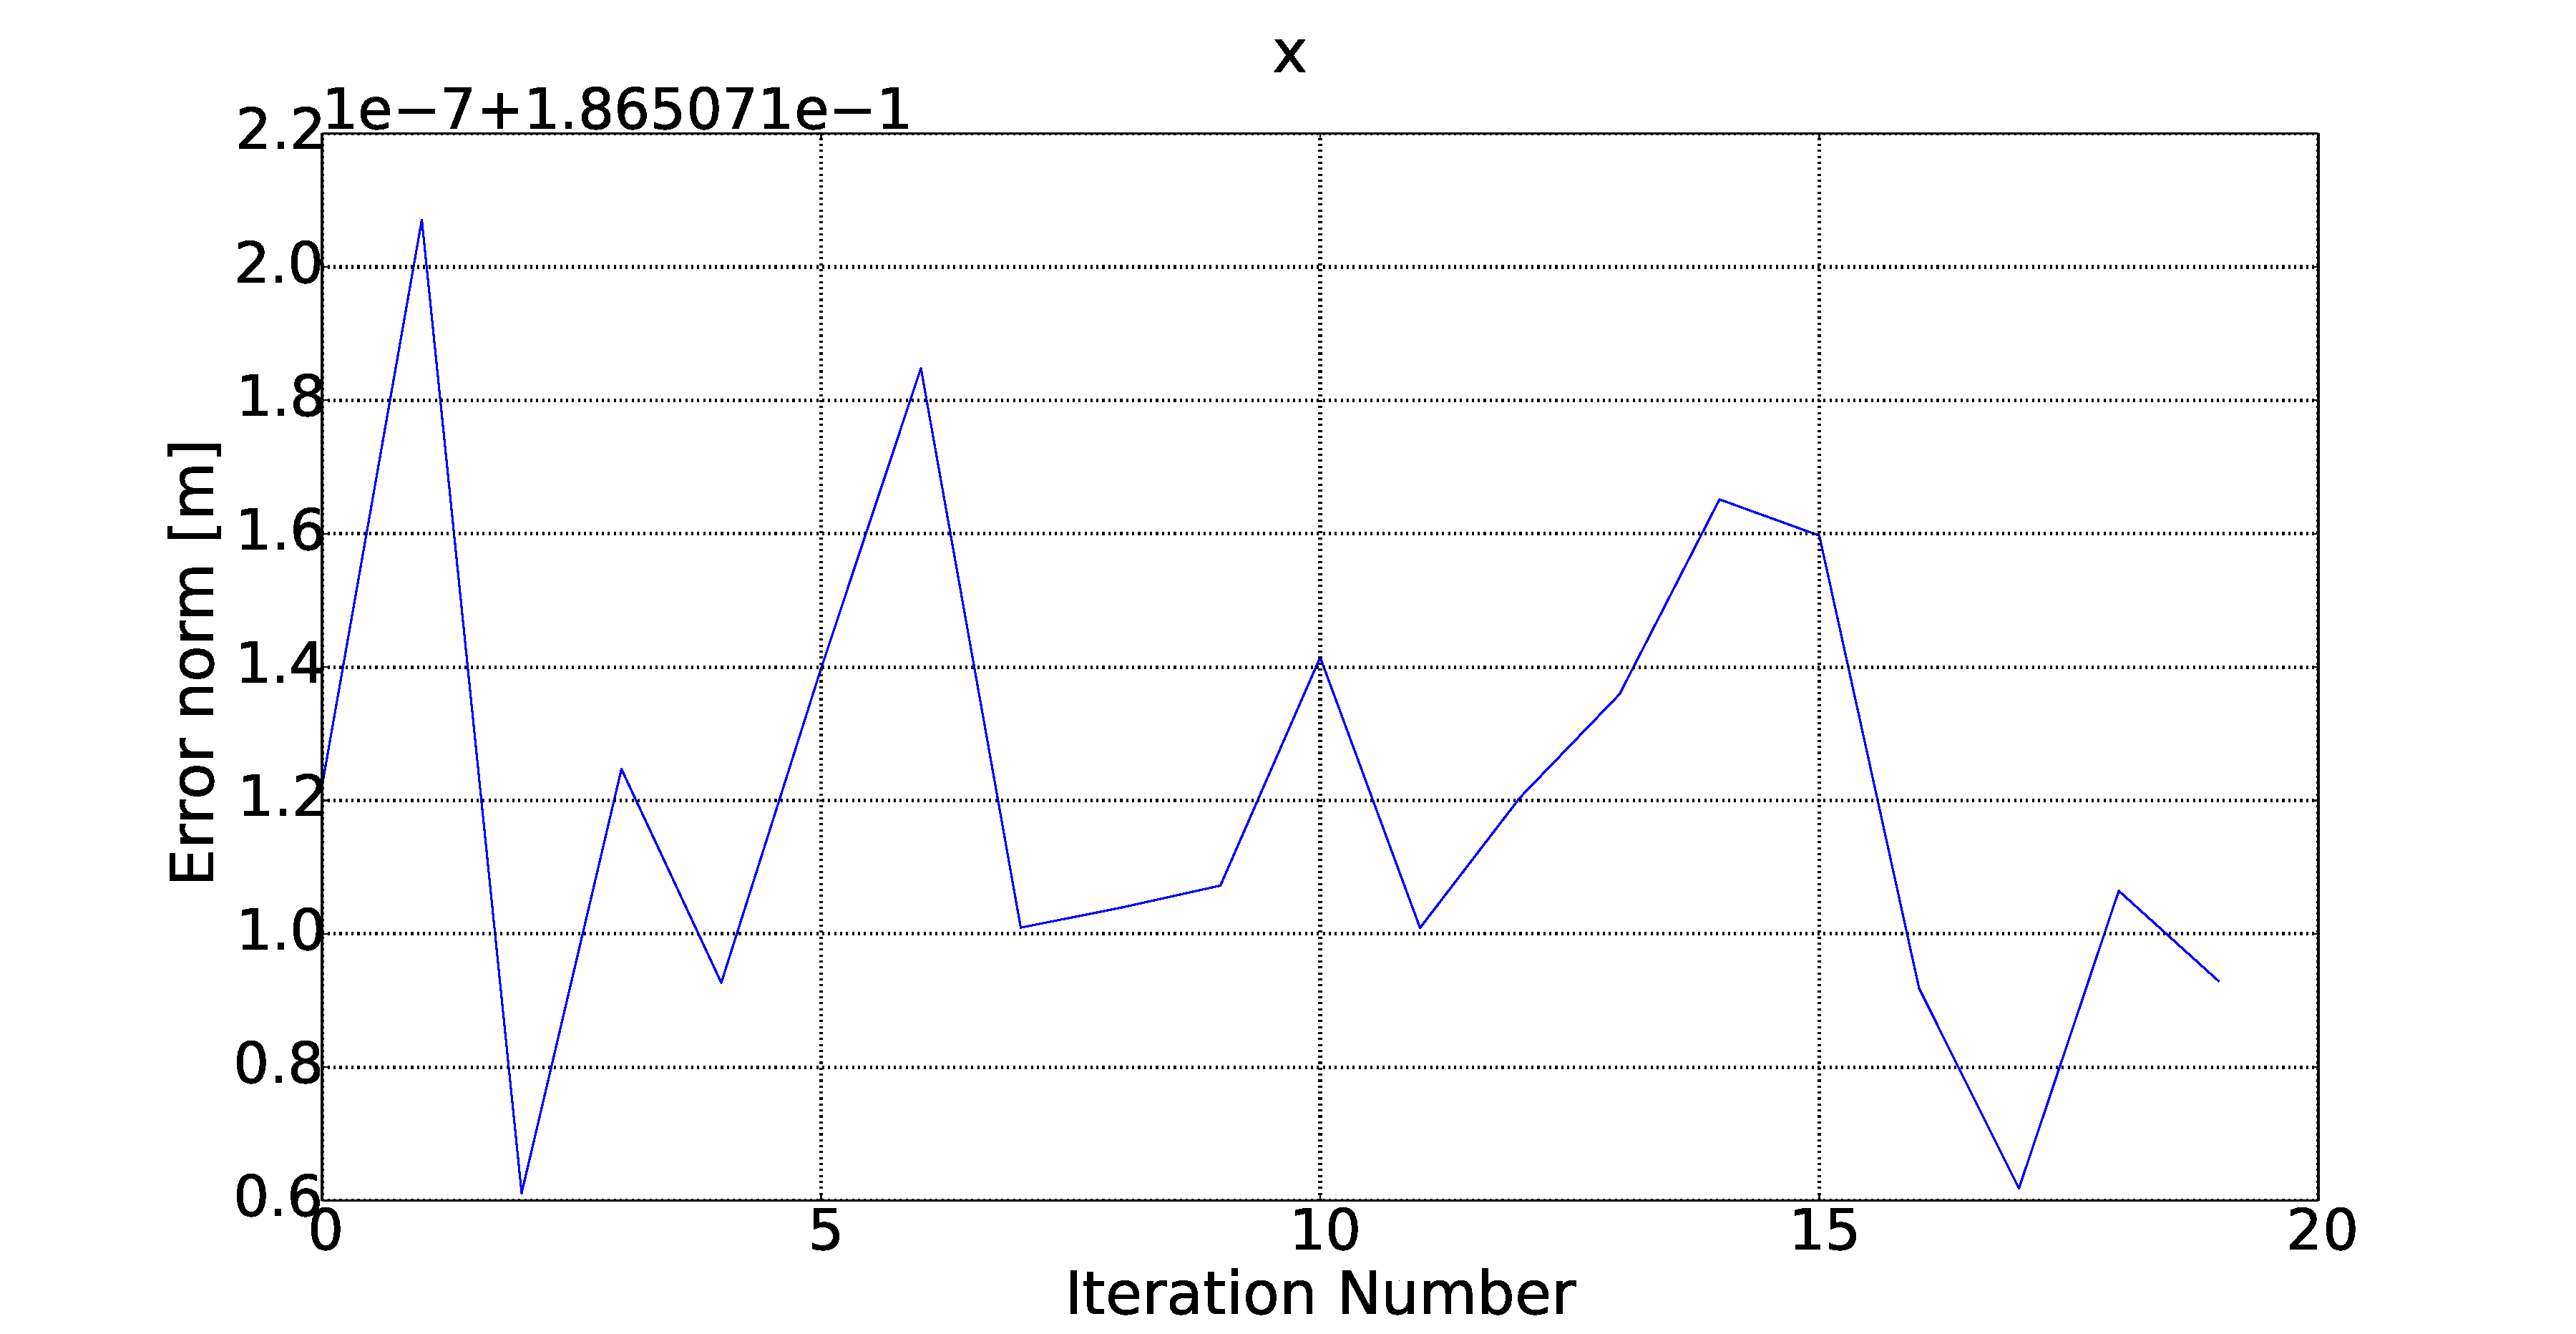
\includegraphics[width=\textwidth]{figures/chapter3/err_x.pdf}
    \caption{Error convergence in the $x$ dimension [m].}
\label{fig:err-convergence-x}
  \end{subfigure}
~
  \begin{subfigure}{0.45\textwidth}
    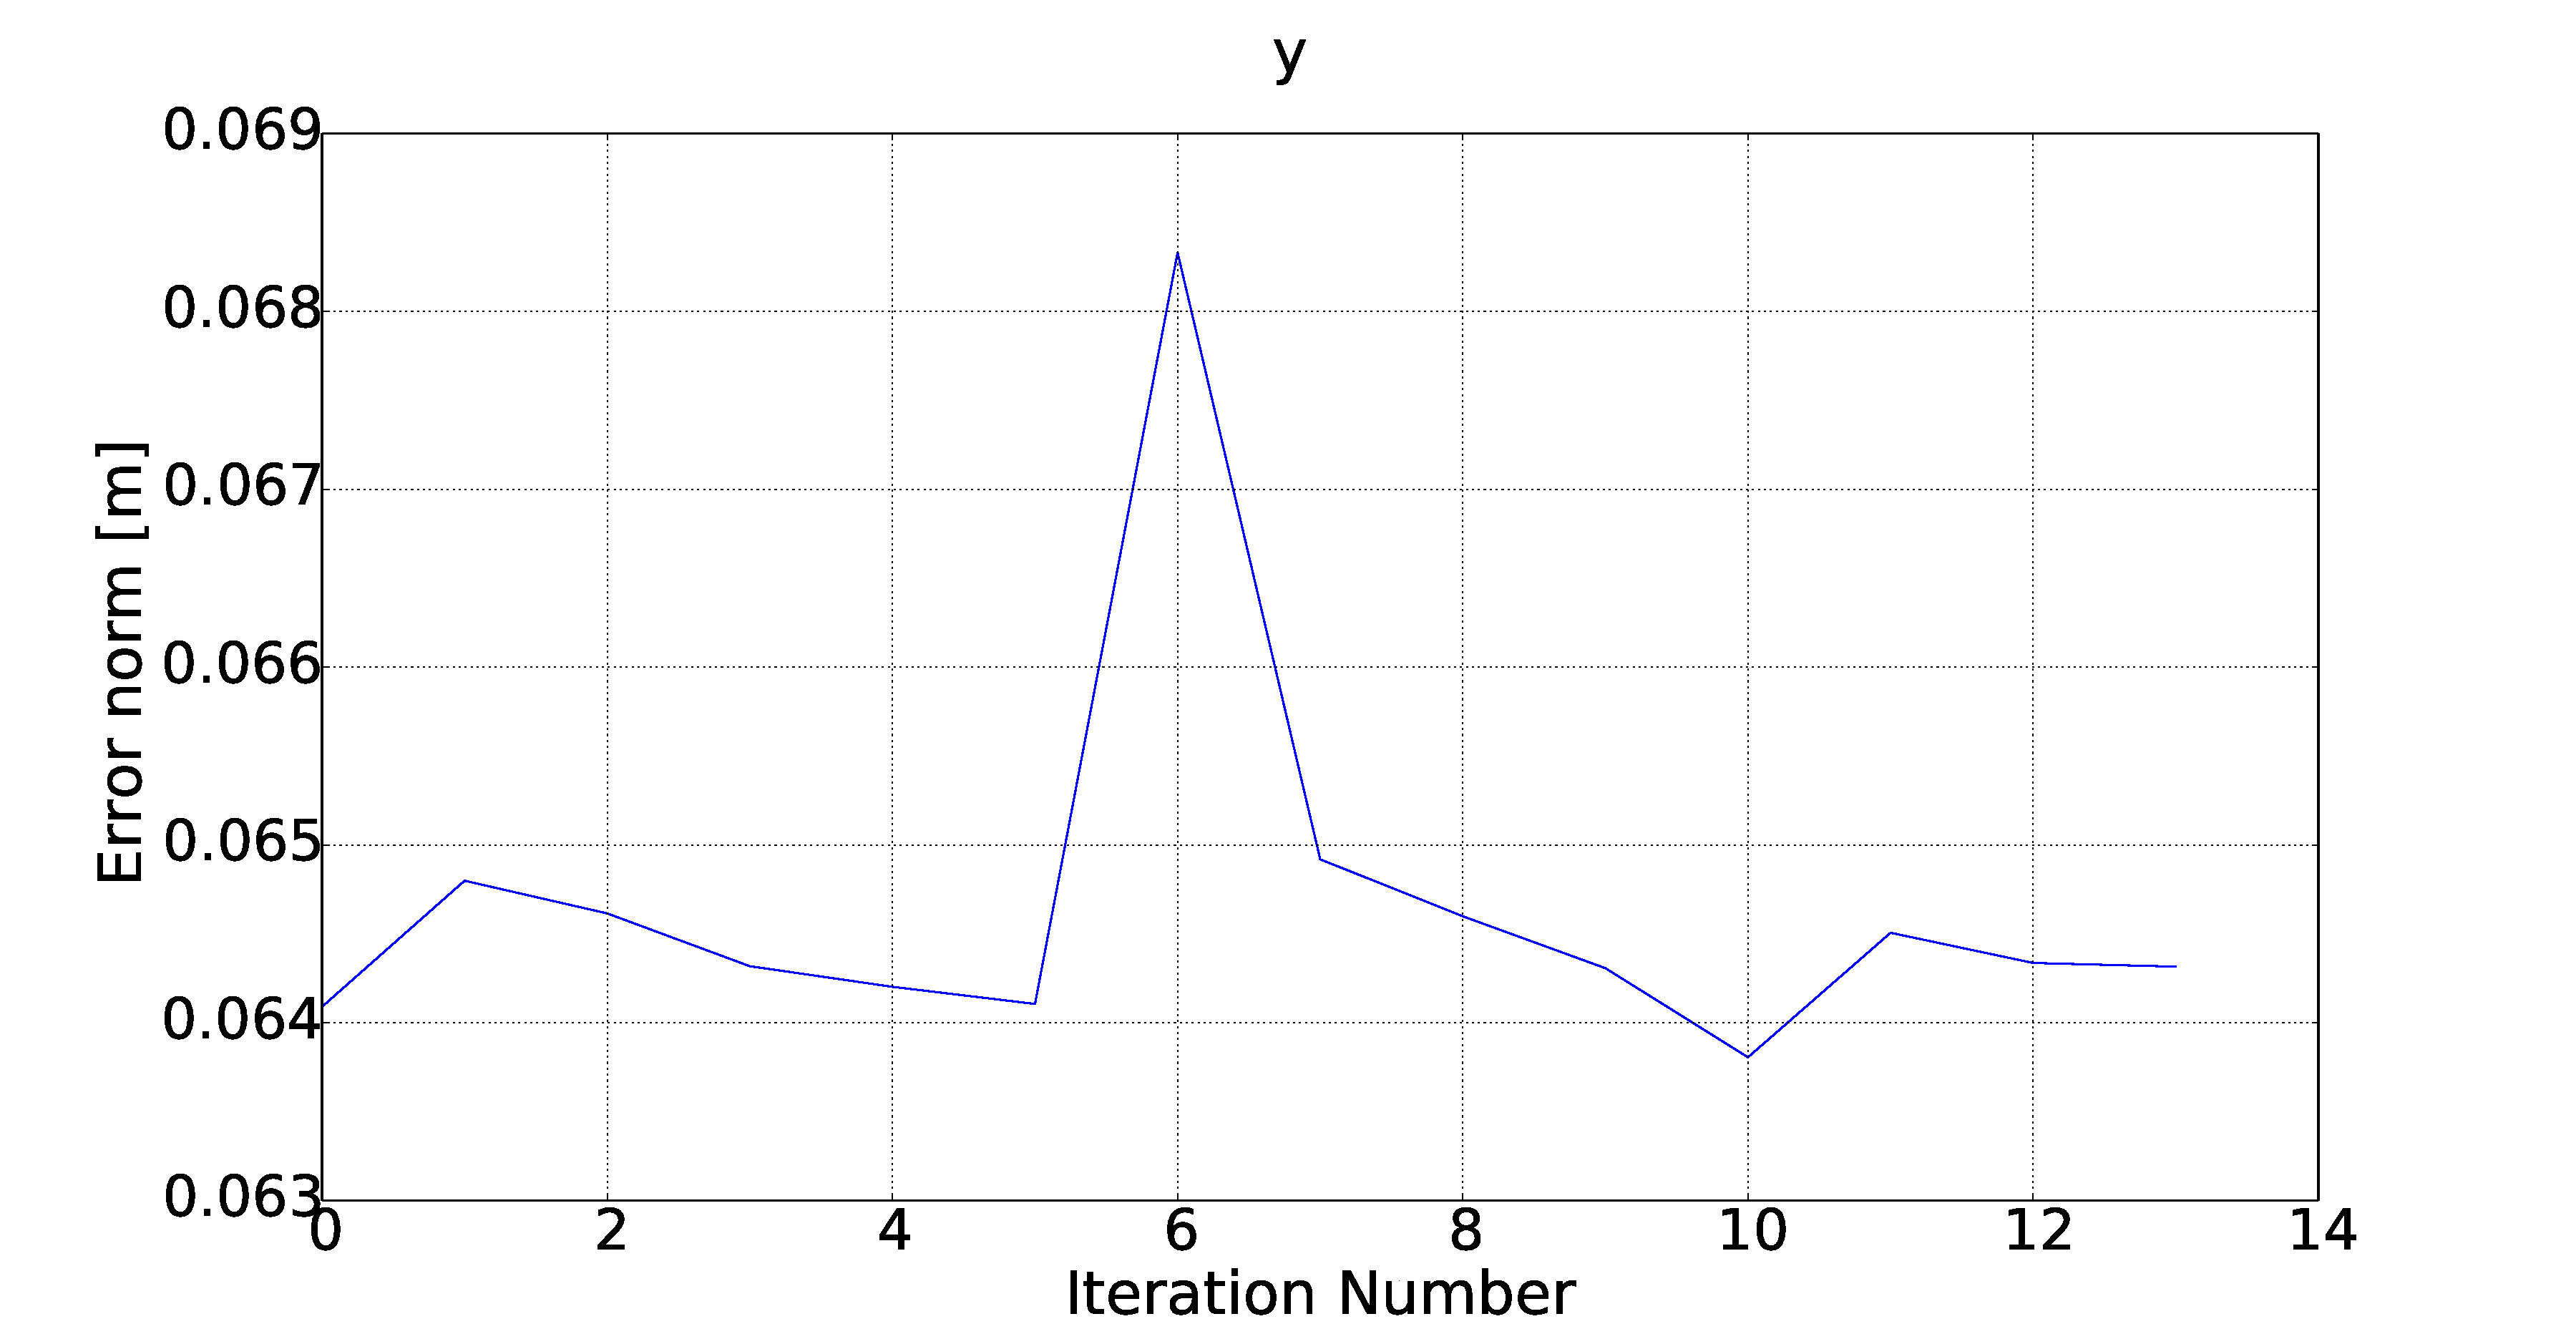
\includegraphics[width=\textwidth]{figures/chapter3/err_y.pdf}
    \caption{Error convergence in the $y$ dimension [m].}
\label{fig:err-convergence-y}
  \end{subfigure}
~
\begin{subfigure}{0.45\textwidth}
    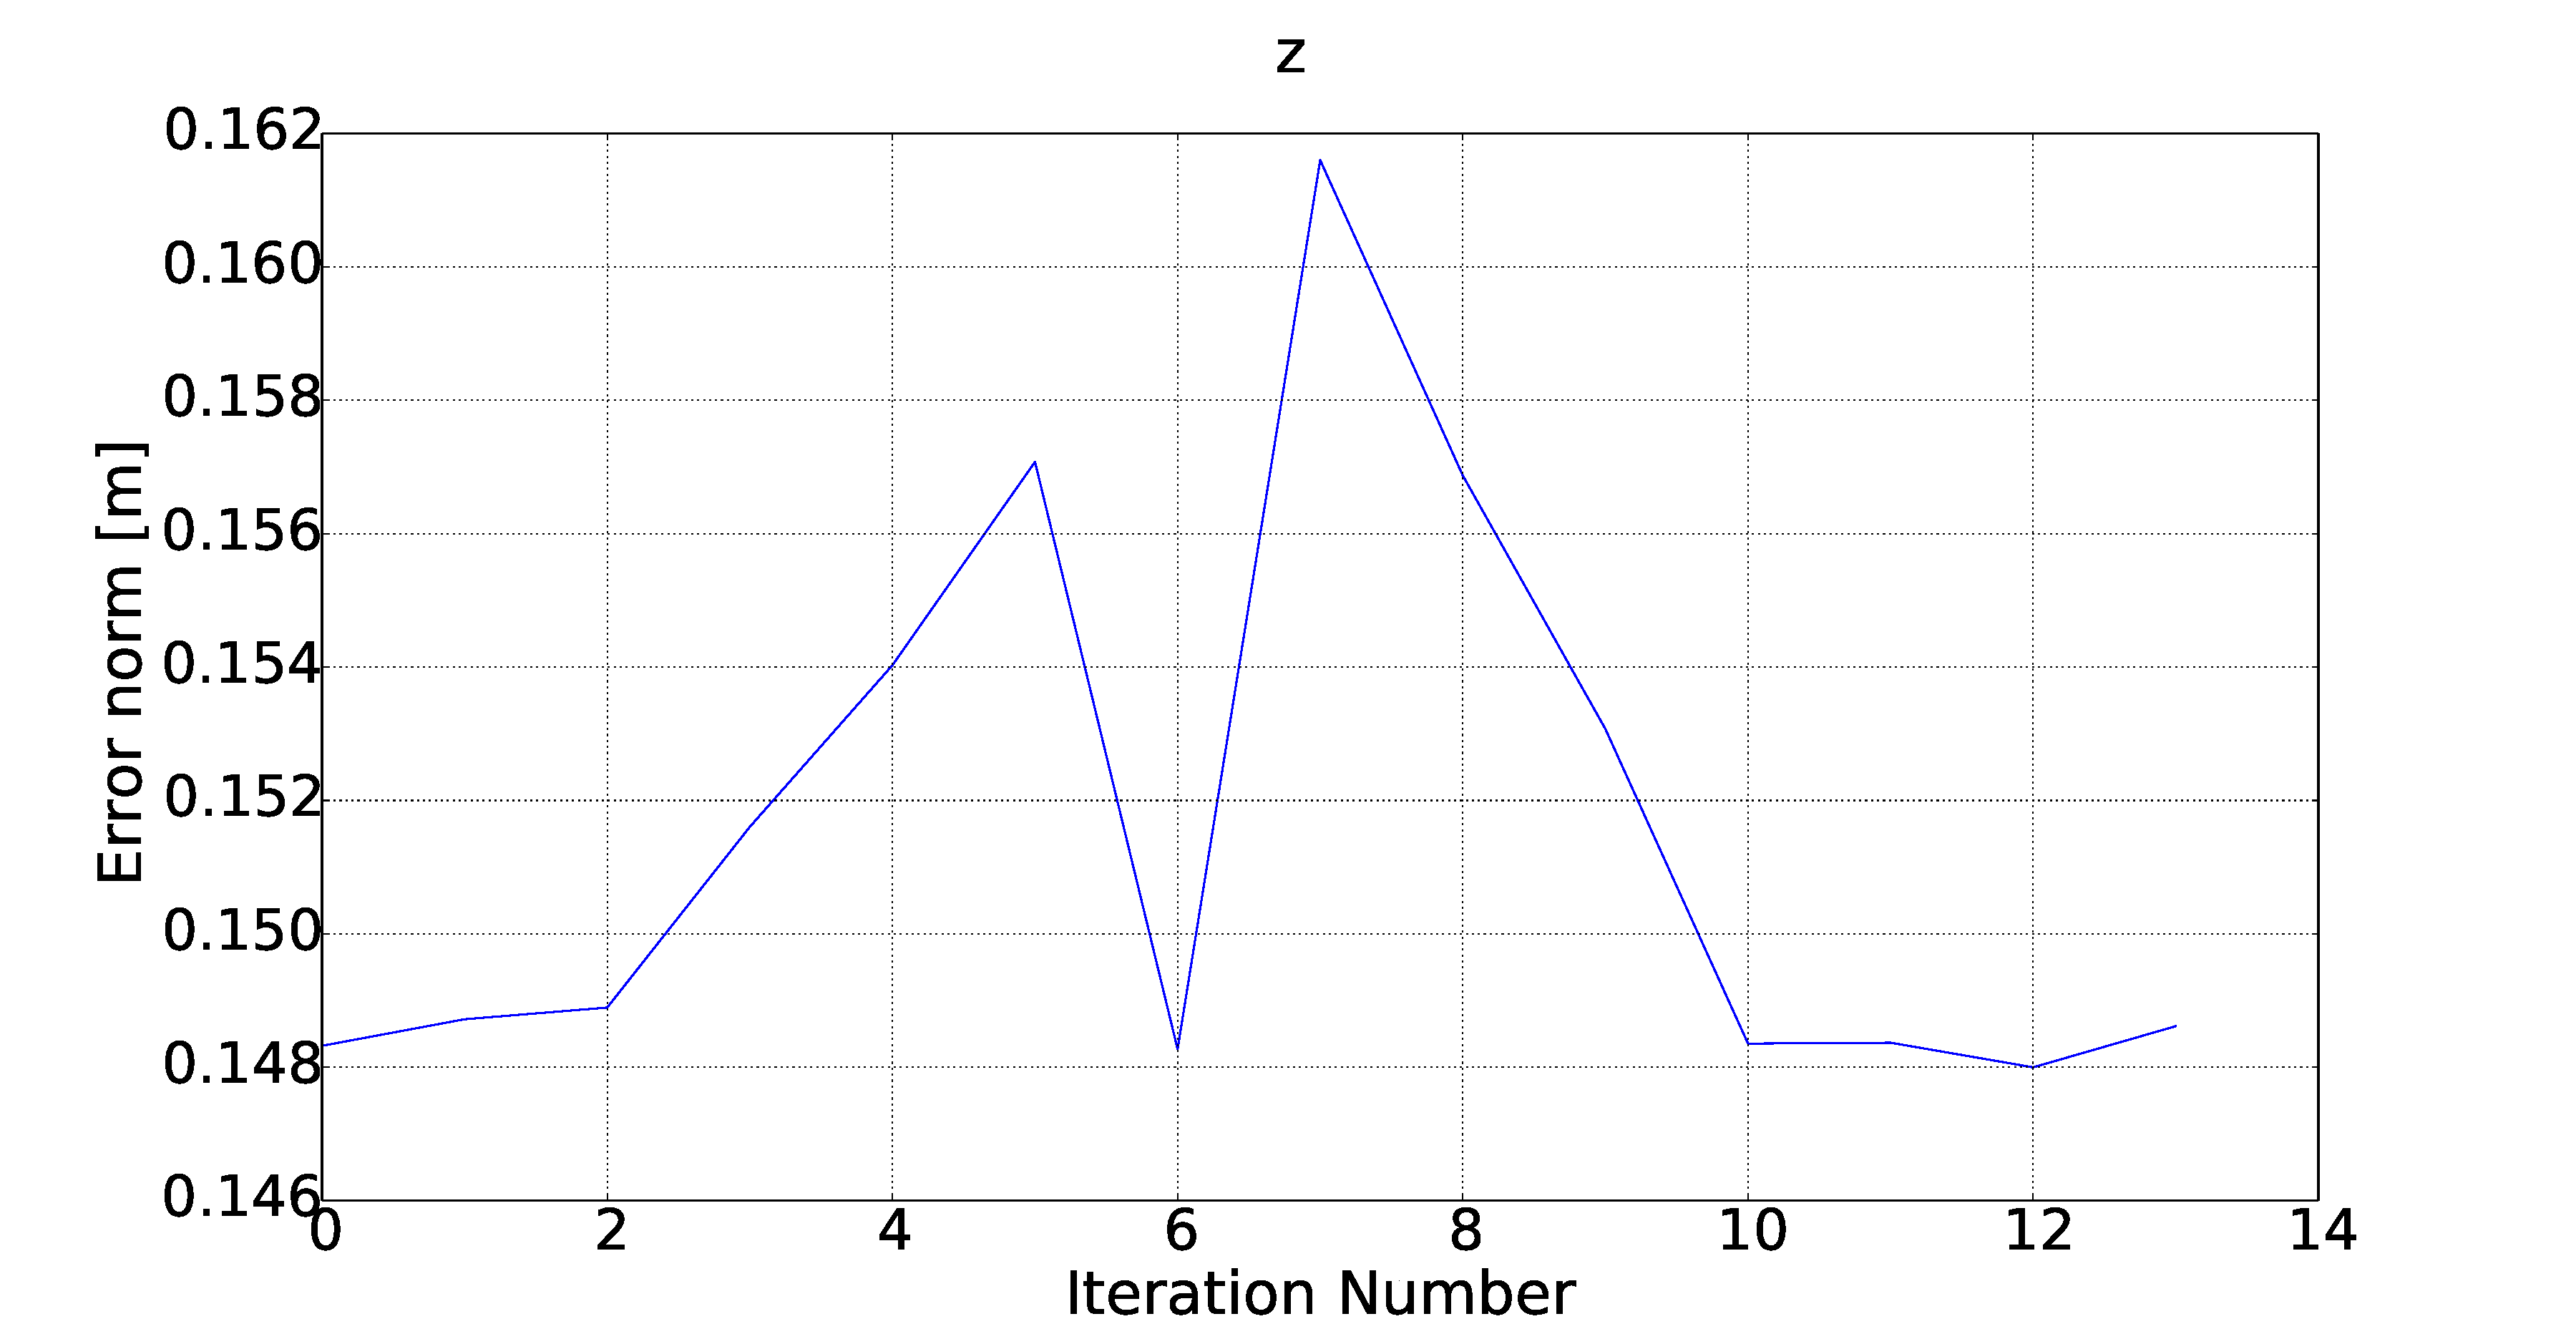
\includegraphics[width=\textwidth]{figures/chapter3/err_z.pdf}
    \caption{Error convergence in the $z$ dimension [m].}
\label{fig:err-convergence-z}
  \end{subfigure}
~
  \begin{subfigure}{0.45\textwidth}
    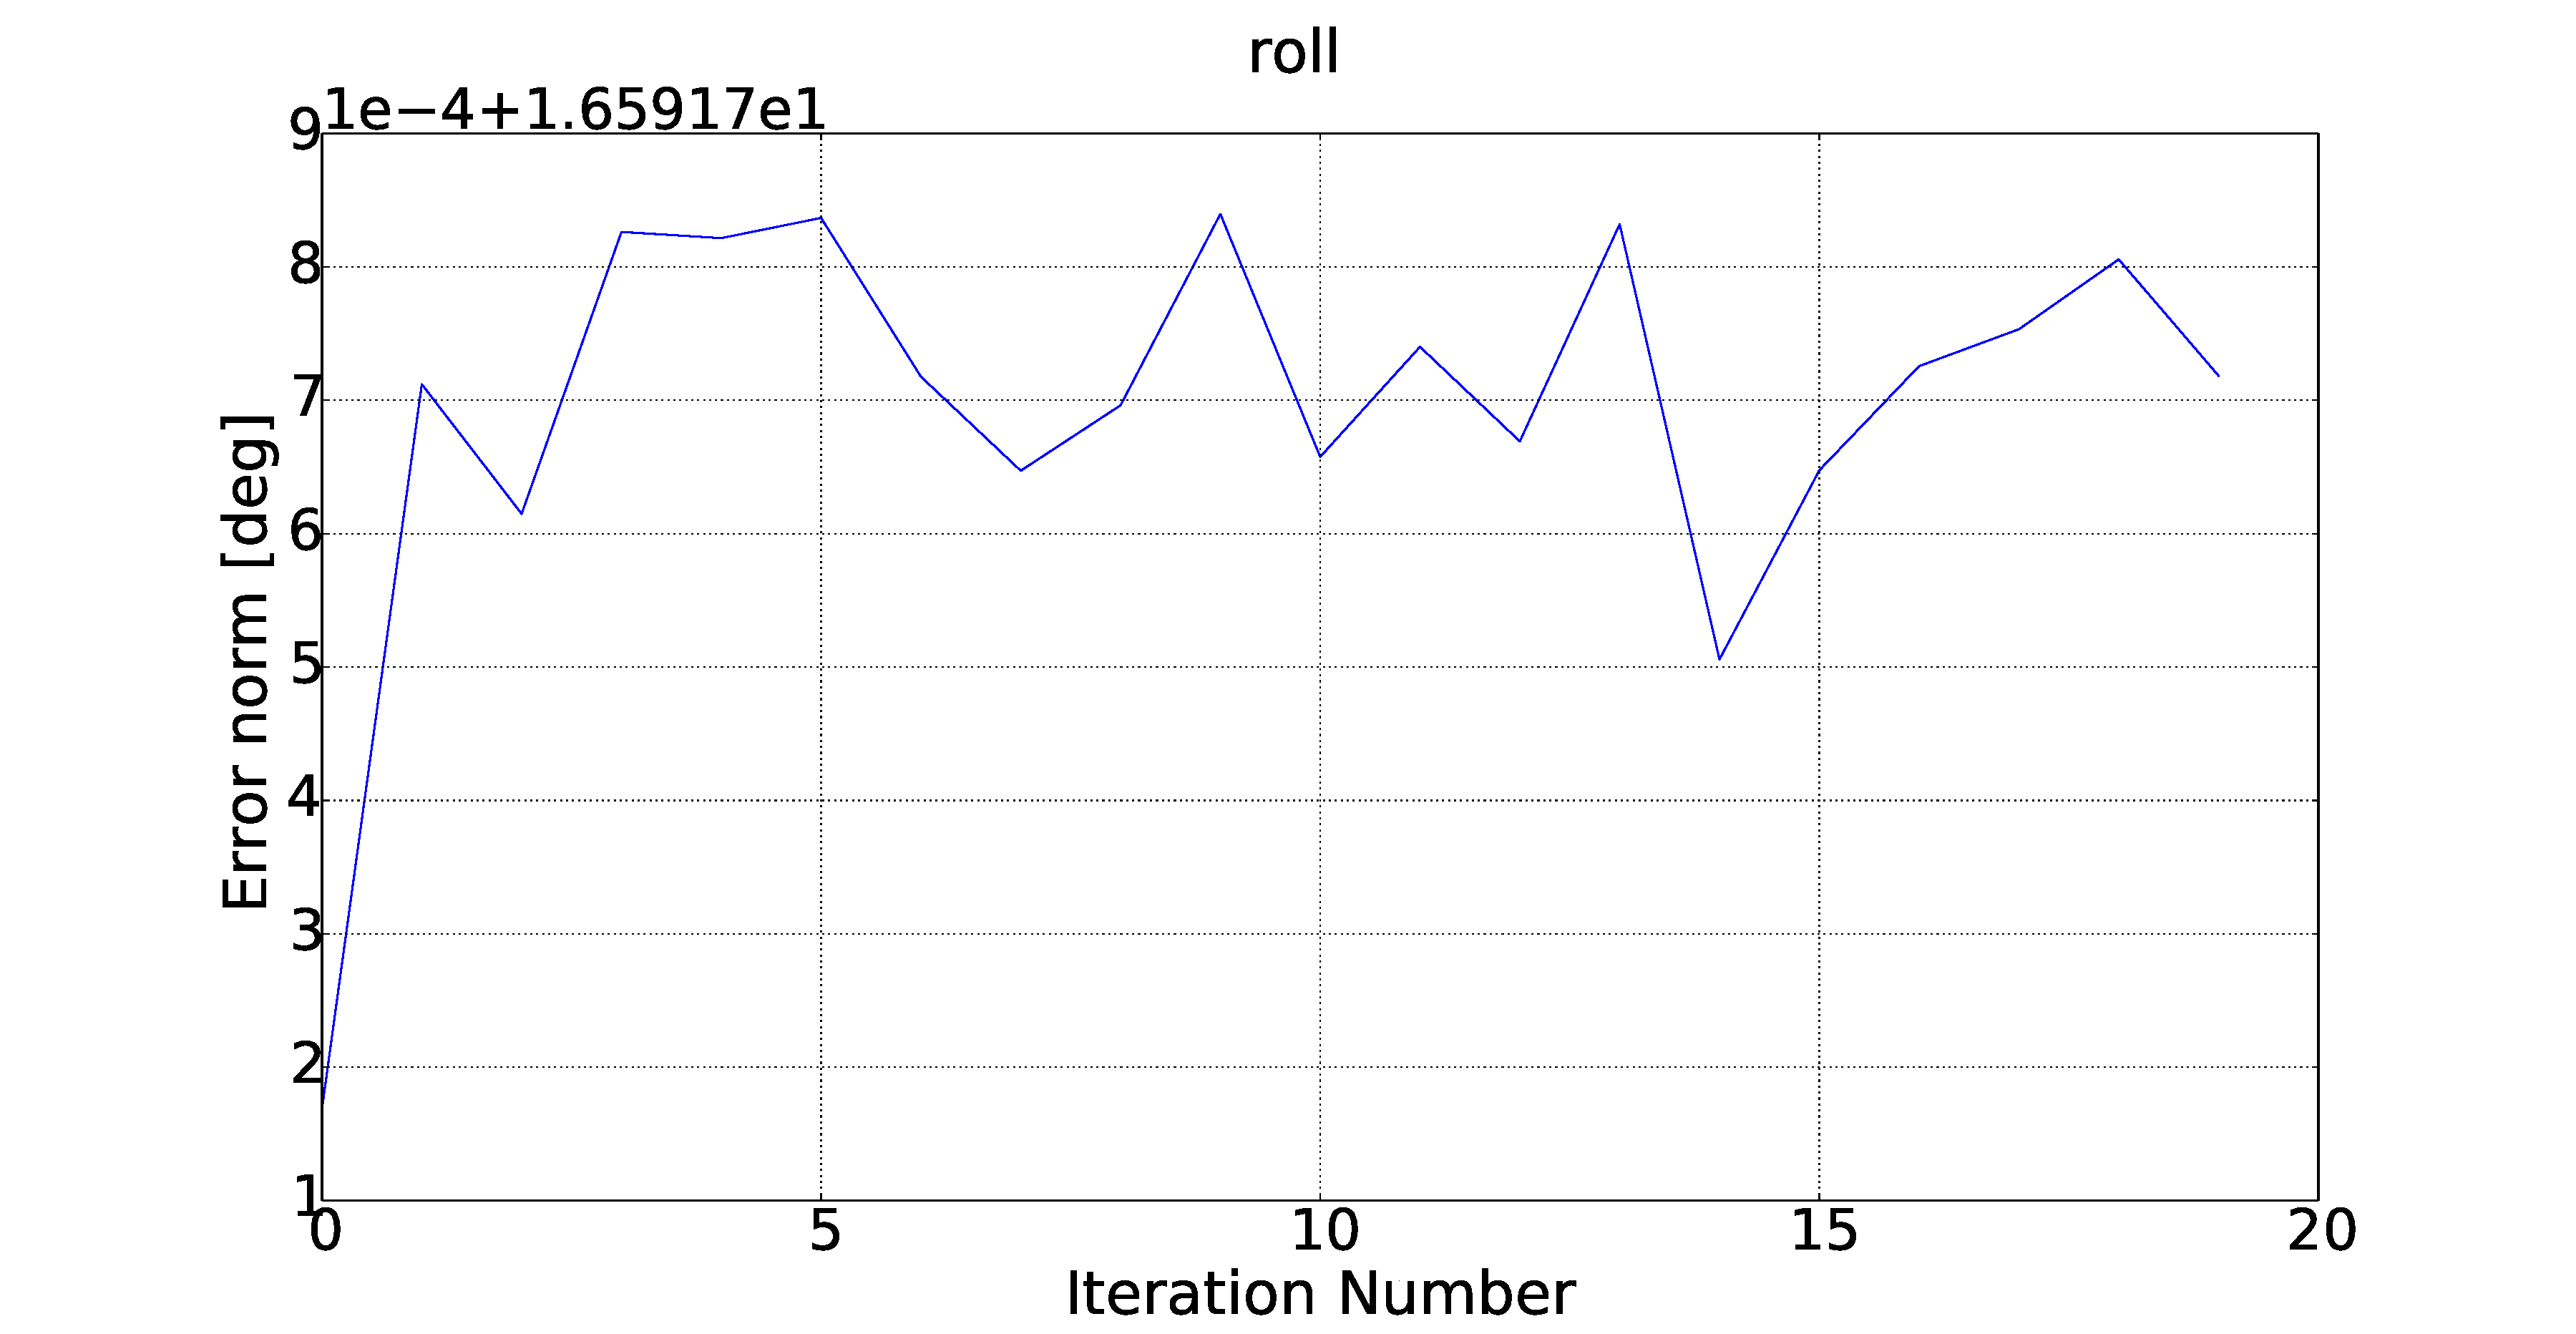
\includegraphics[width=\textwidth]{figures/chapter3/err_roll.pdf}
    \caption{Error convergence in the $\theta$ dimension [degrees].}
\label{fig:err-convergence-roll}
  \end{subfigure}
~
  \begin{subfigure}{0.45\textwidth}
    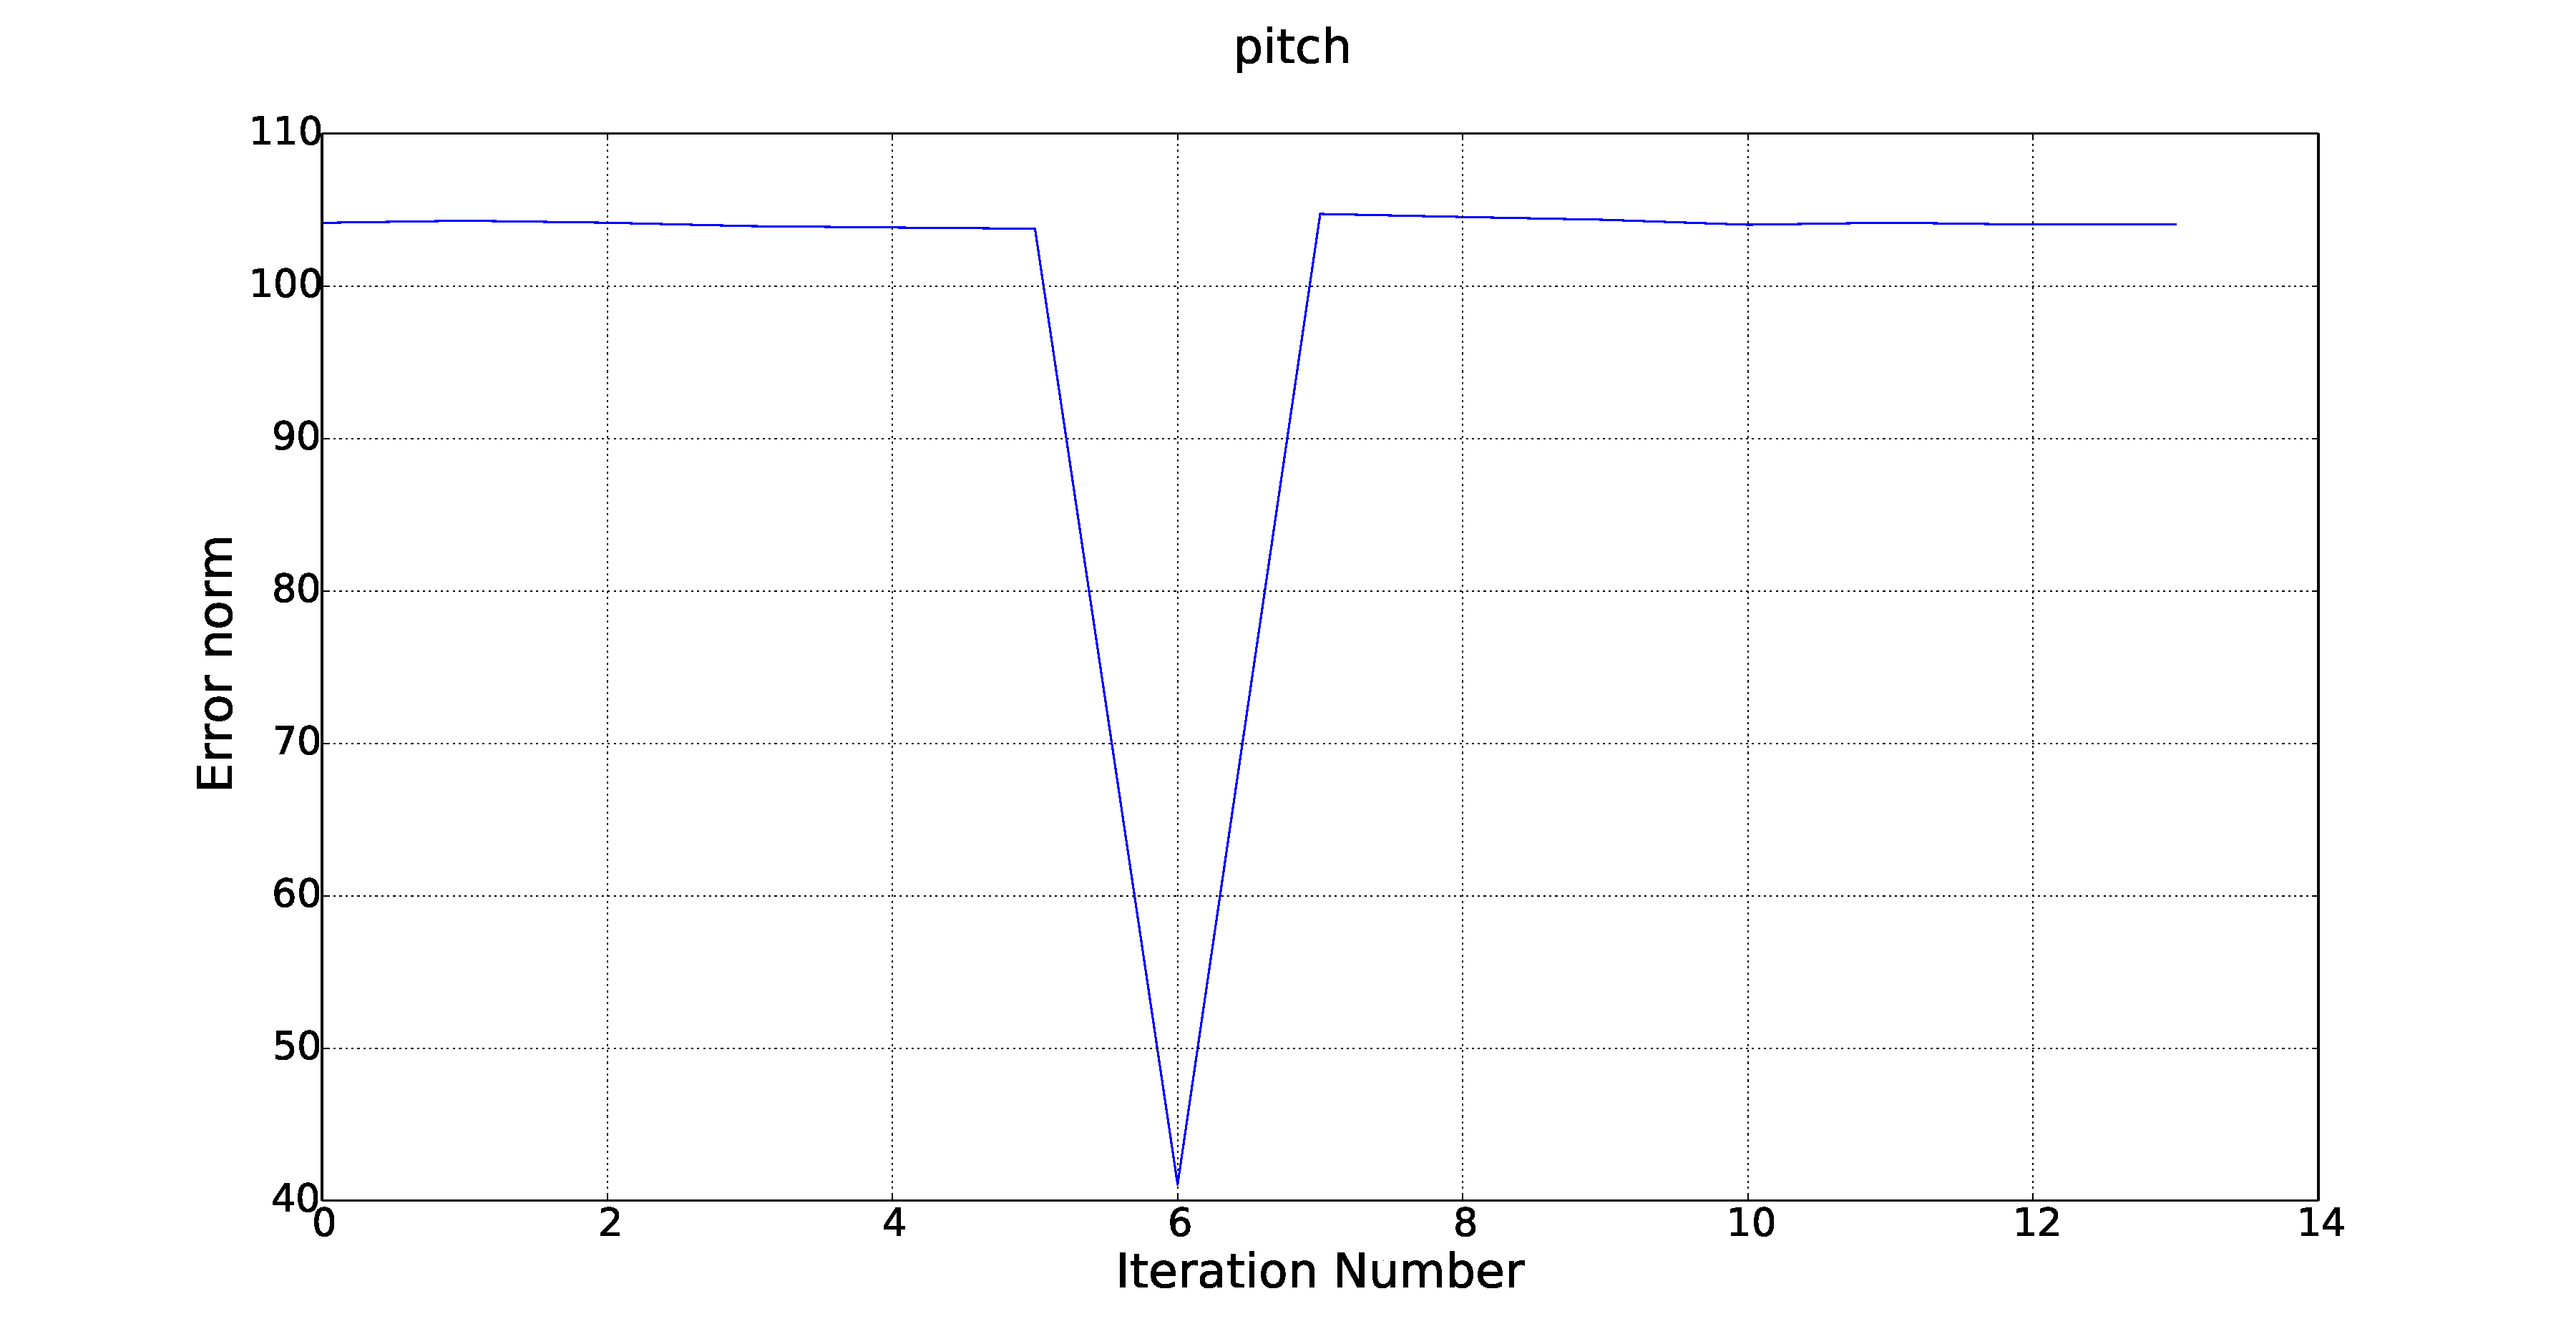
\includegraphics[width=\textwidth]{figures/chapter3/err_pitch.pdf}
    \caption{Error convergence in the $\phi$ dimension [degrees].}
\label{fig:err-convergence-pitch}
  \end{subfigure}
~
  \begin{subfigure}{0.45\textwidth}
    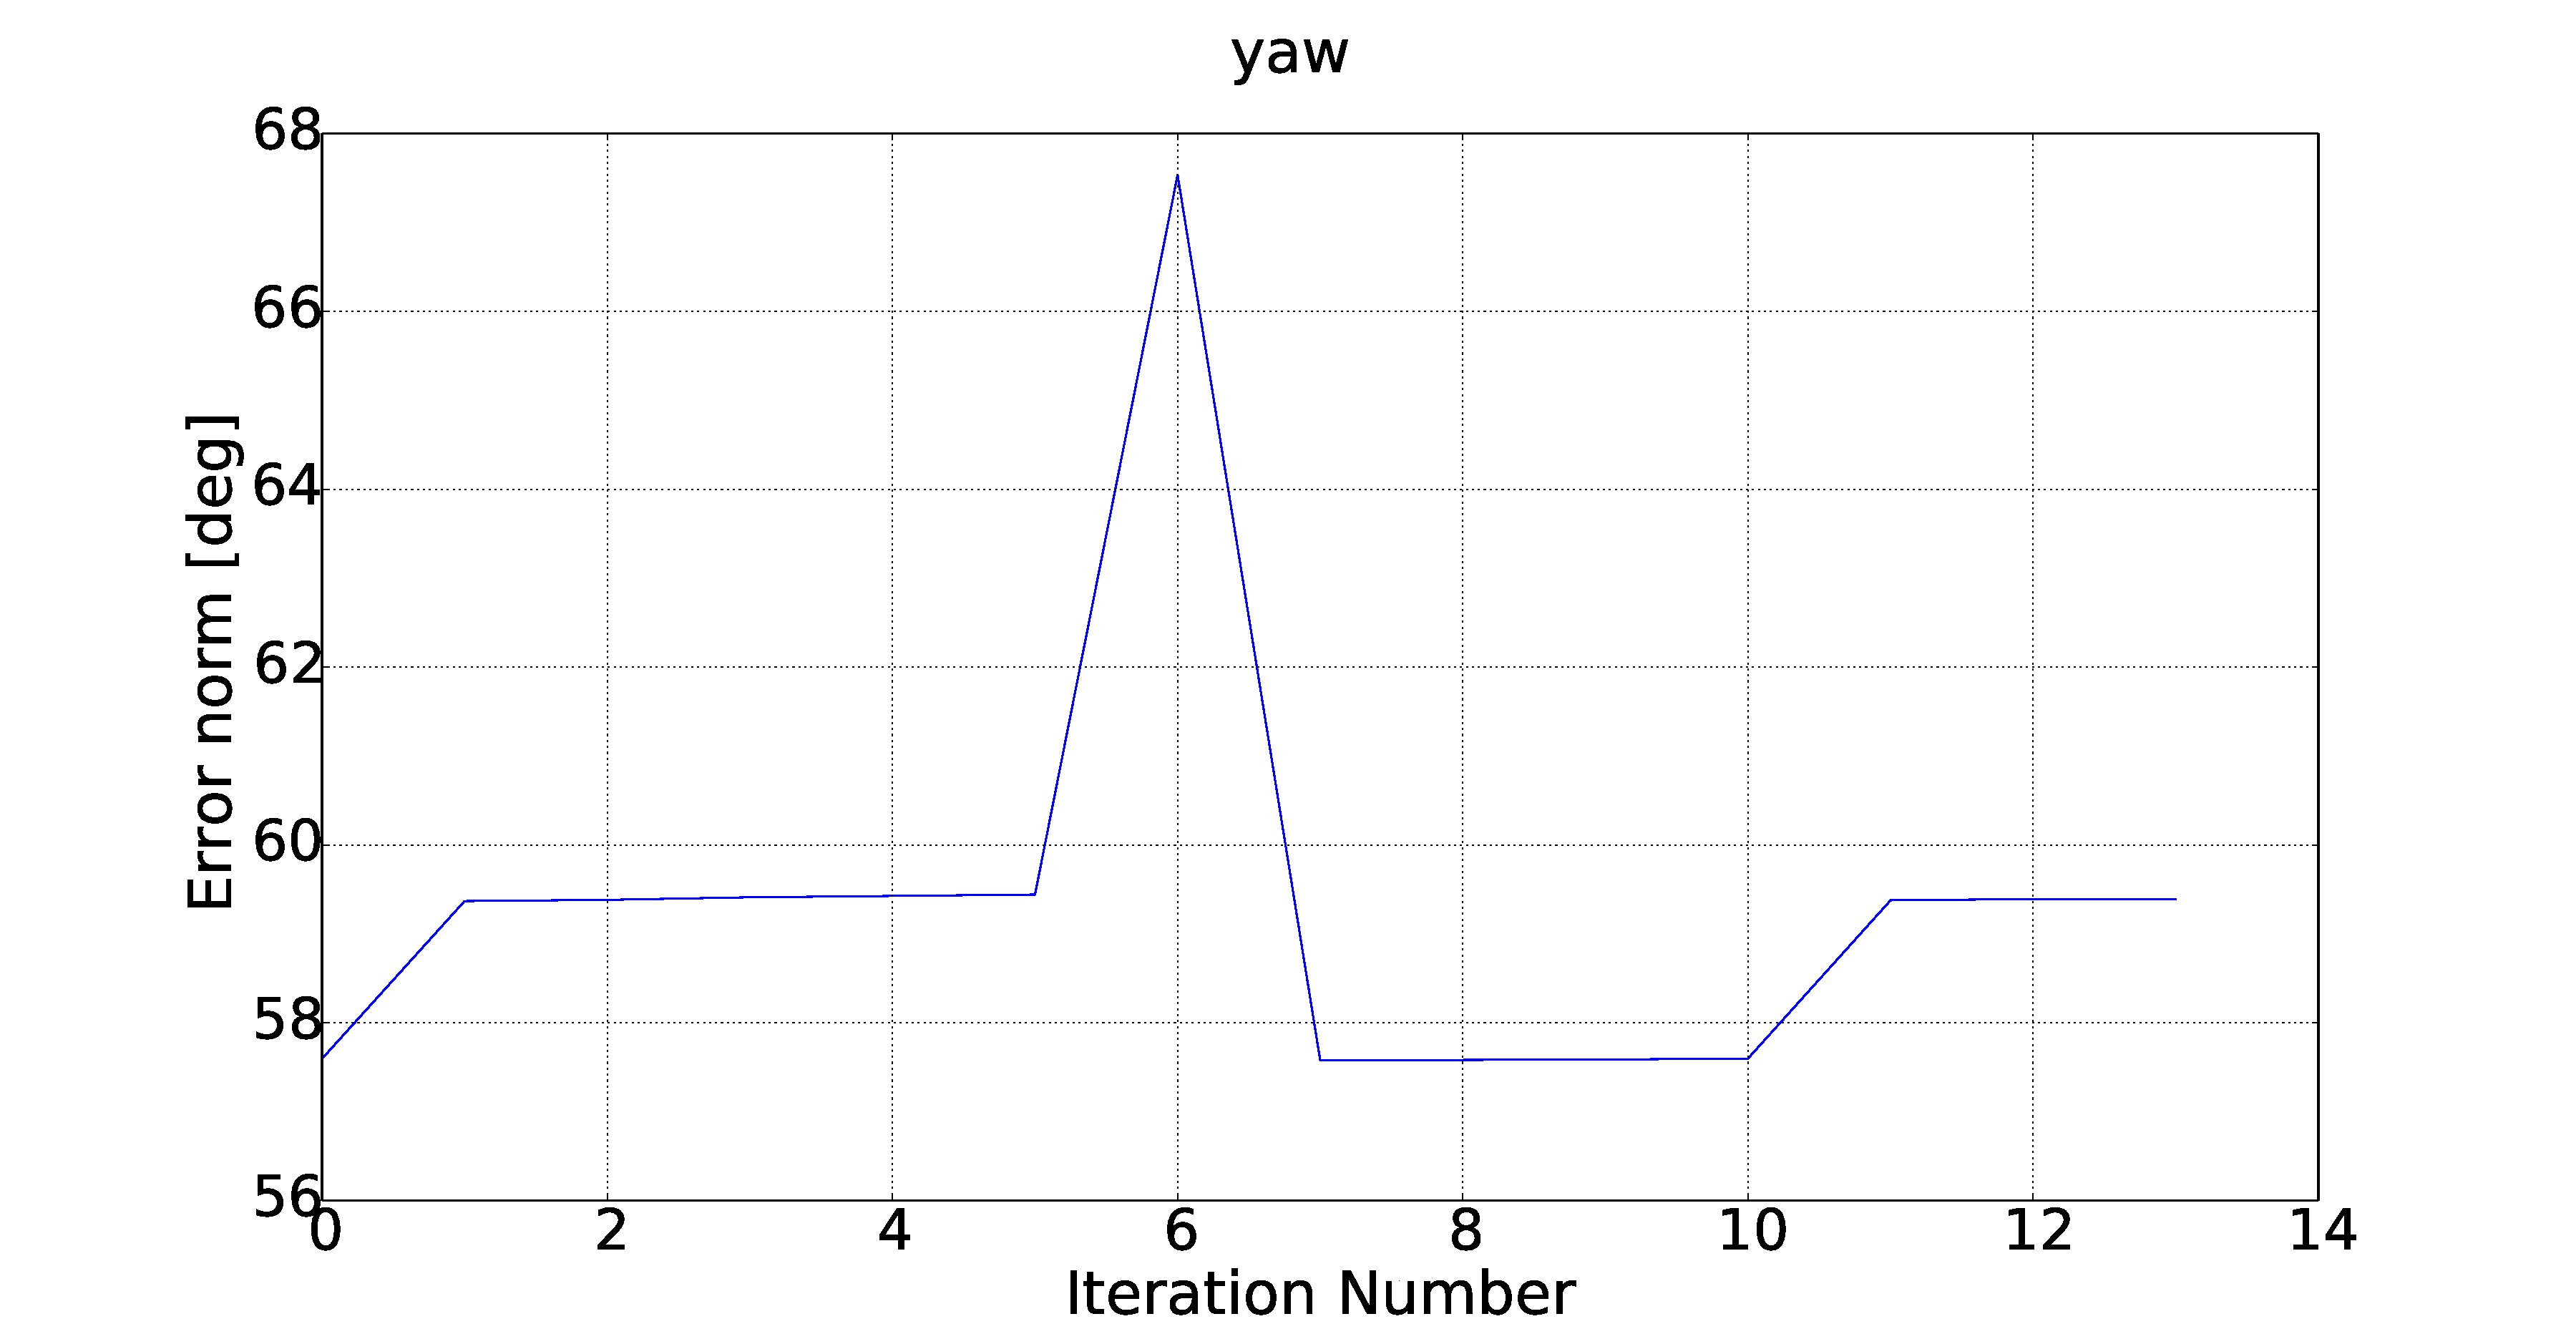
\includegraphics[width=\textwidth]{figures/chapter3/err_yaw.pdf}
    \caption{Error convergence in the $\psi$ dimension [degrees].}
\label{fig:err-convergence-psi}
  \end{subfigure}
  \caption[Plots showing error convergence for the optimsation procedure.]{Plots showing the error in each dimension during for each iteration of the error minimisation procedure.}
  \label{fig:err-convergence}
\end{figure*}

The graphs in Figure~\ref{fig:err-convergence} show that the error gets reduced in the $x$ and $z$ dimensions, while it gets worse in the $y$ and all of the orientation angle dimensions. 

The errors in the orientation angle dimensions are growing, since they carry no weight in the optimisation cost function. As for the growing error in the $y$ dimension, closer inspection of the graph shows that the $y$ dimension initially has the smallest error. It may be argued that since all three translation dimensions carry equal weight in the optimisation cost function, the $x$ and $z$ dimensions are being reduced at the cost of the error in the $y$ dimension. 

\subsection{Test for Normality}
\label{sec:err-norm-test}

HERSIEN DIE PLOTTE EN ALS MEME

To check if the error in $\bm{\epsilon}$ is indeed normally distributed, as assumed in Equation~\ref{eq:chap3-eq2-offset}, frequency histograms of the error matrix $\bm{\epsilon}$ in all six dimensions are plotted along with a normal distribution drawn using each dimension's mean and standard deviation. A $\chi^2$ (chi-squared) test could also have been used. However, it was found that the sample size of the data set was too large and it is known that some skewness in the data can have a large impact on the $\chi^2$ probability estimate CITE???. Therefore, a graphical approach was taken to determining if the errors are normally distributed around zero. 

Figure~\ref{fig:err-norm} shows the frequency histogram plots of the CVS measurement errors in the six dimensions. A normal distribution, using the averages and standard deviations from the data set, are superimposed to illustrate the normal distribution of the data.

\begin{figure*}
  \begin{subfigure}{0.45\textwidth}
    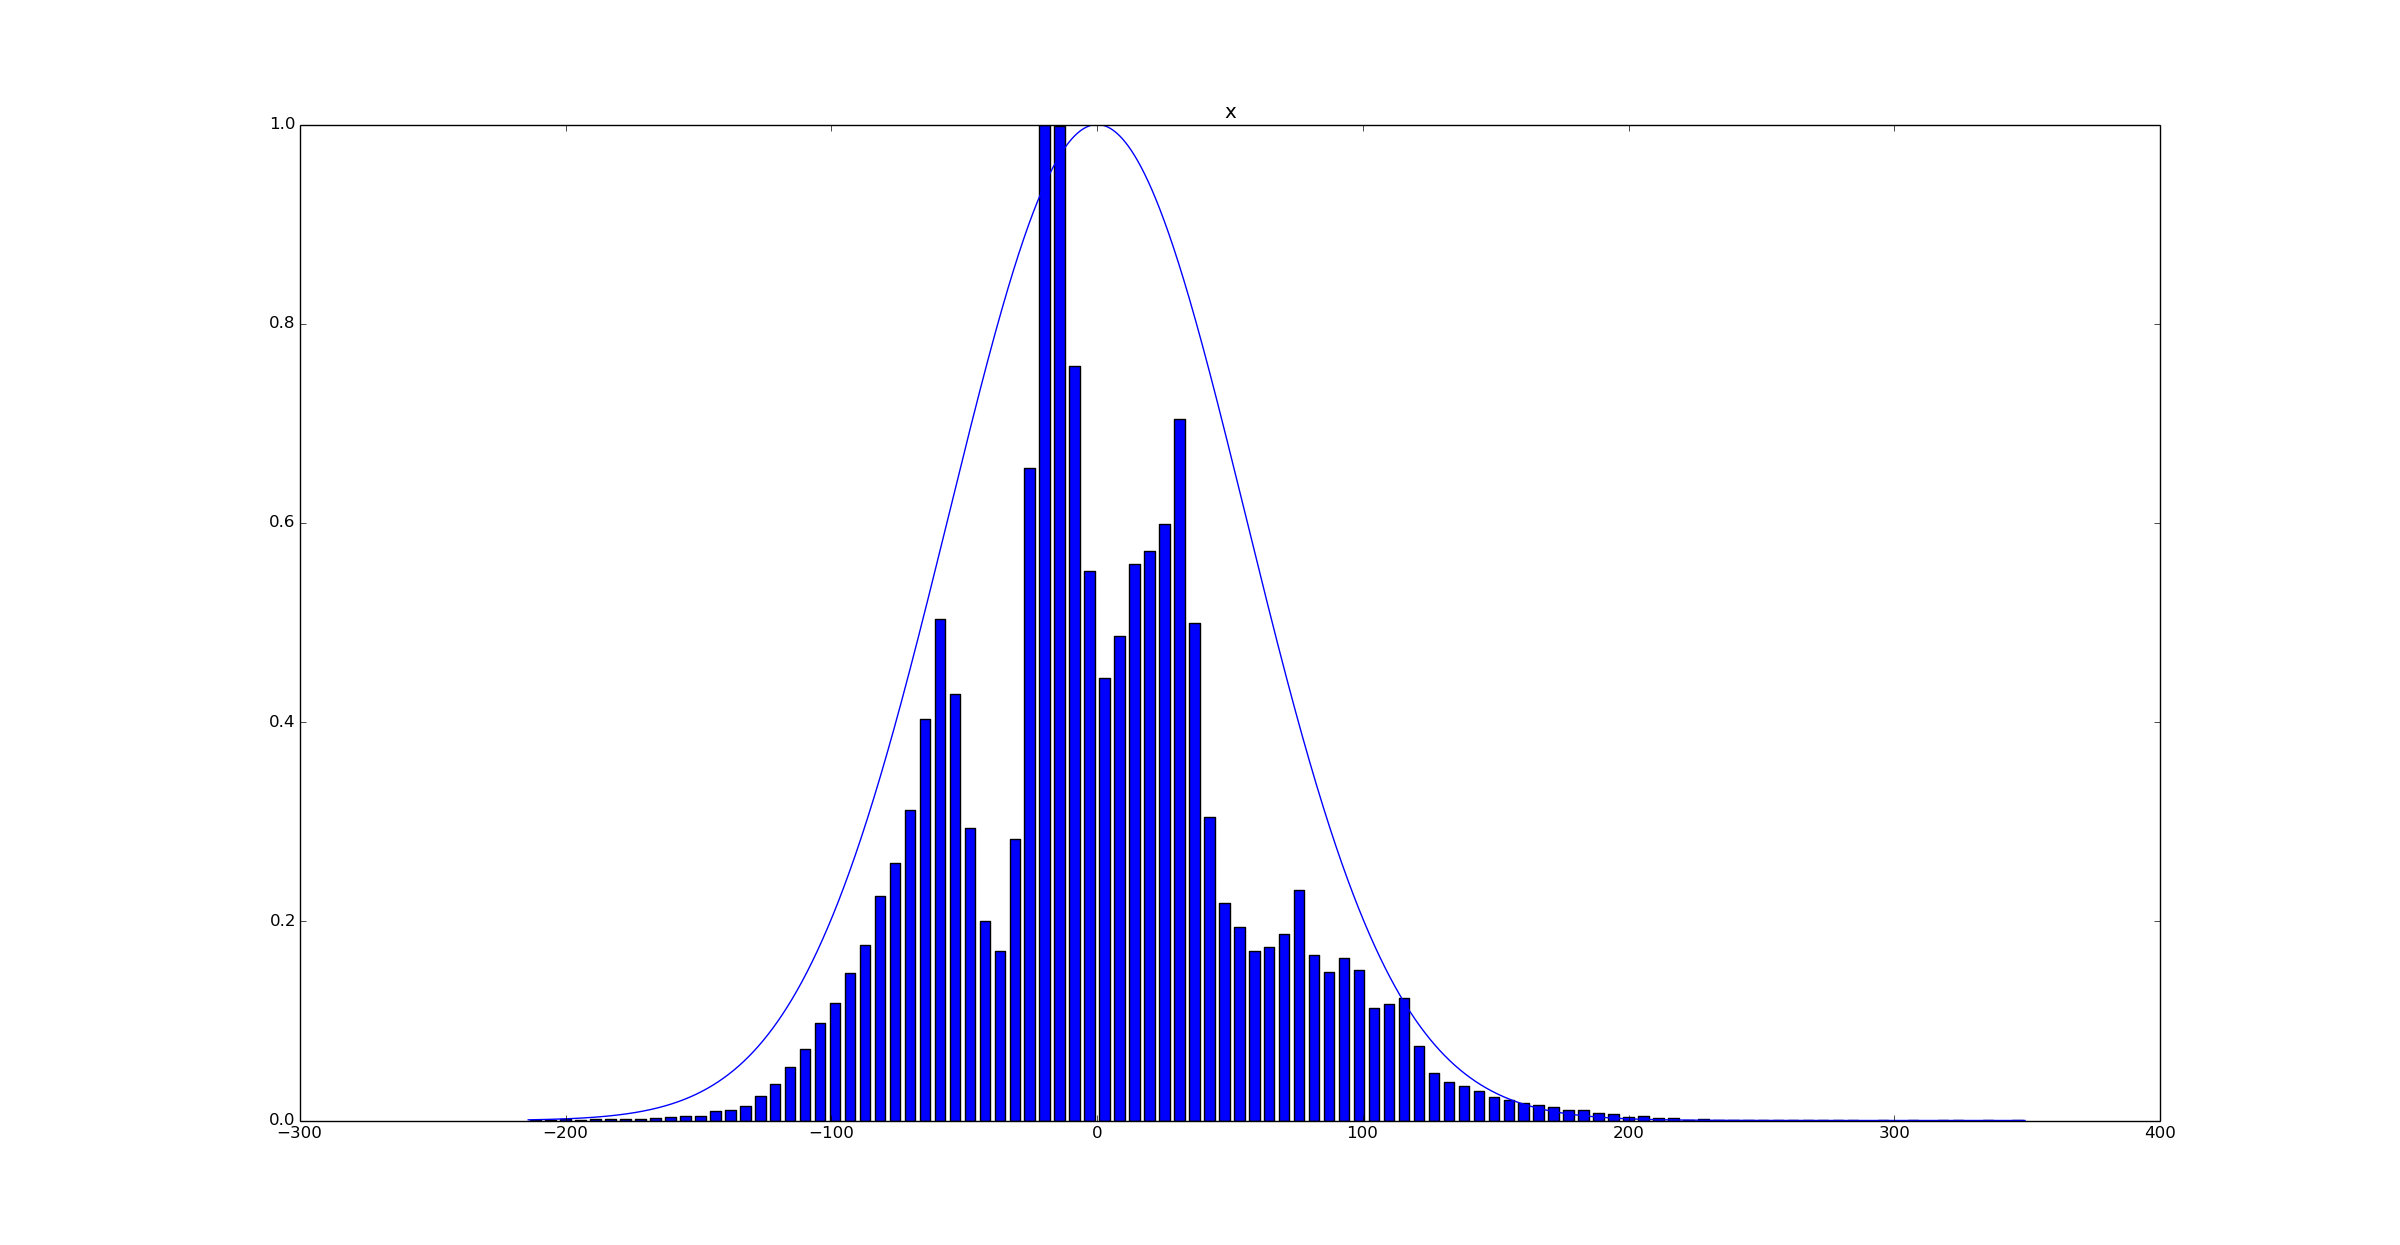
\includegraphics[width=\textwidth]{figures/chapter3/norm_x}
    \caption{Histogram of the error in the $x$ dimension with a mean of $-5.17\mu$m and a standard deviation of 293mm.}
  \end{subfigure}
~
  \begin{subfigure}{0.45\textwidth}
     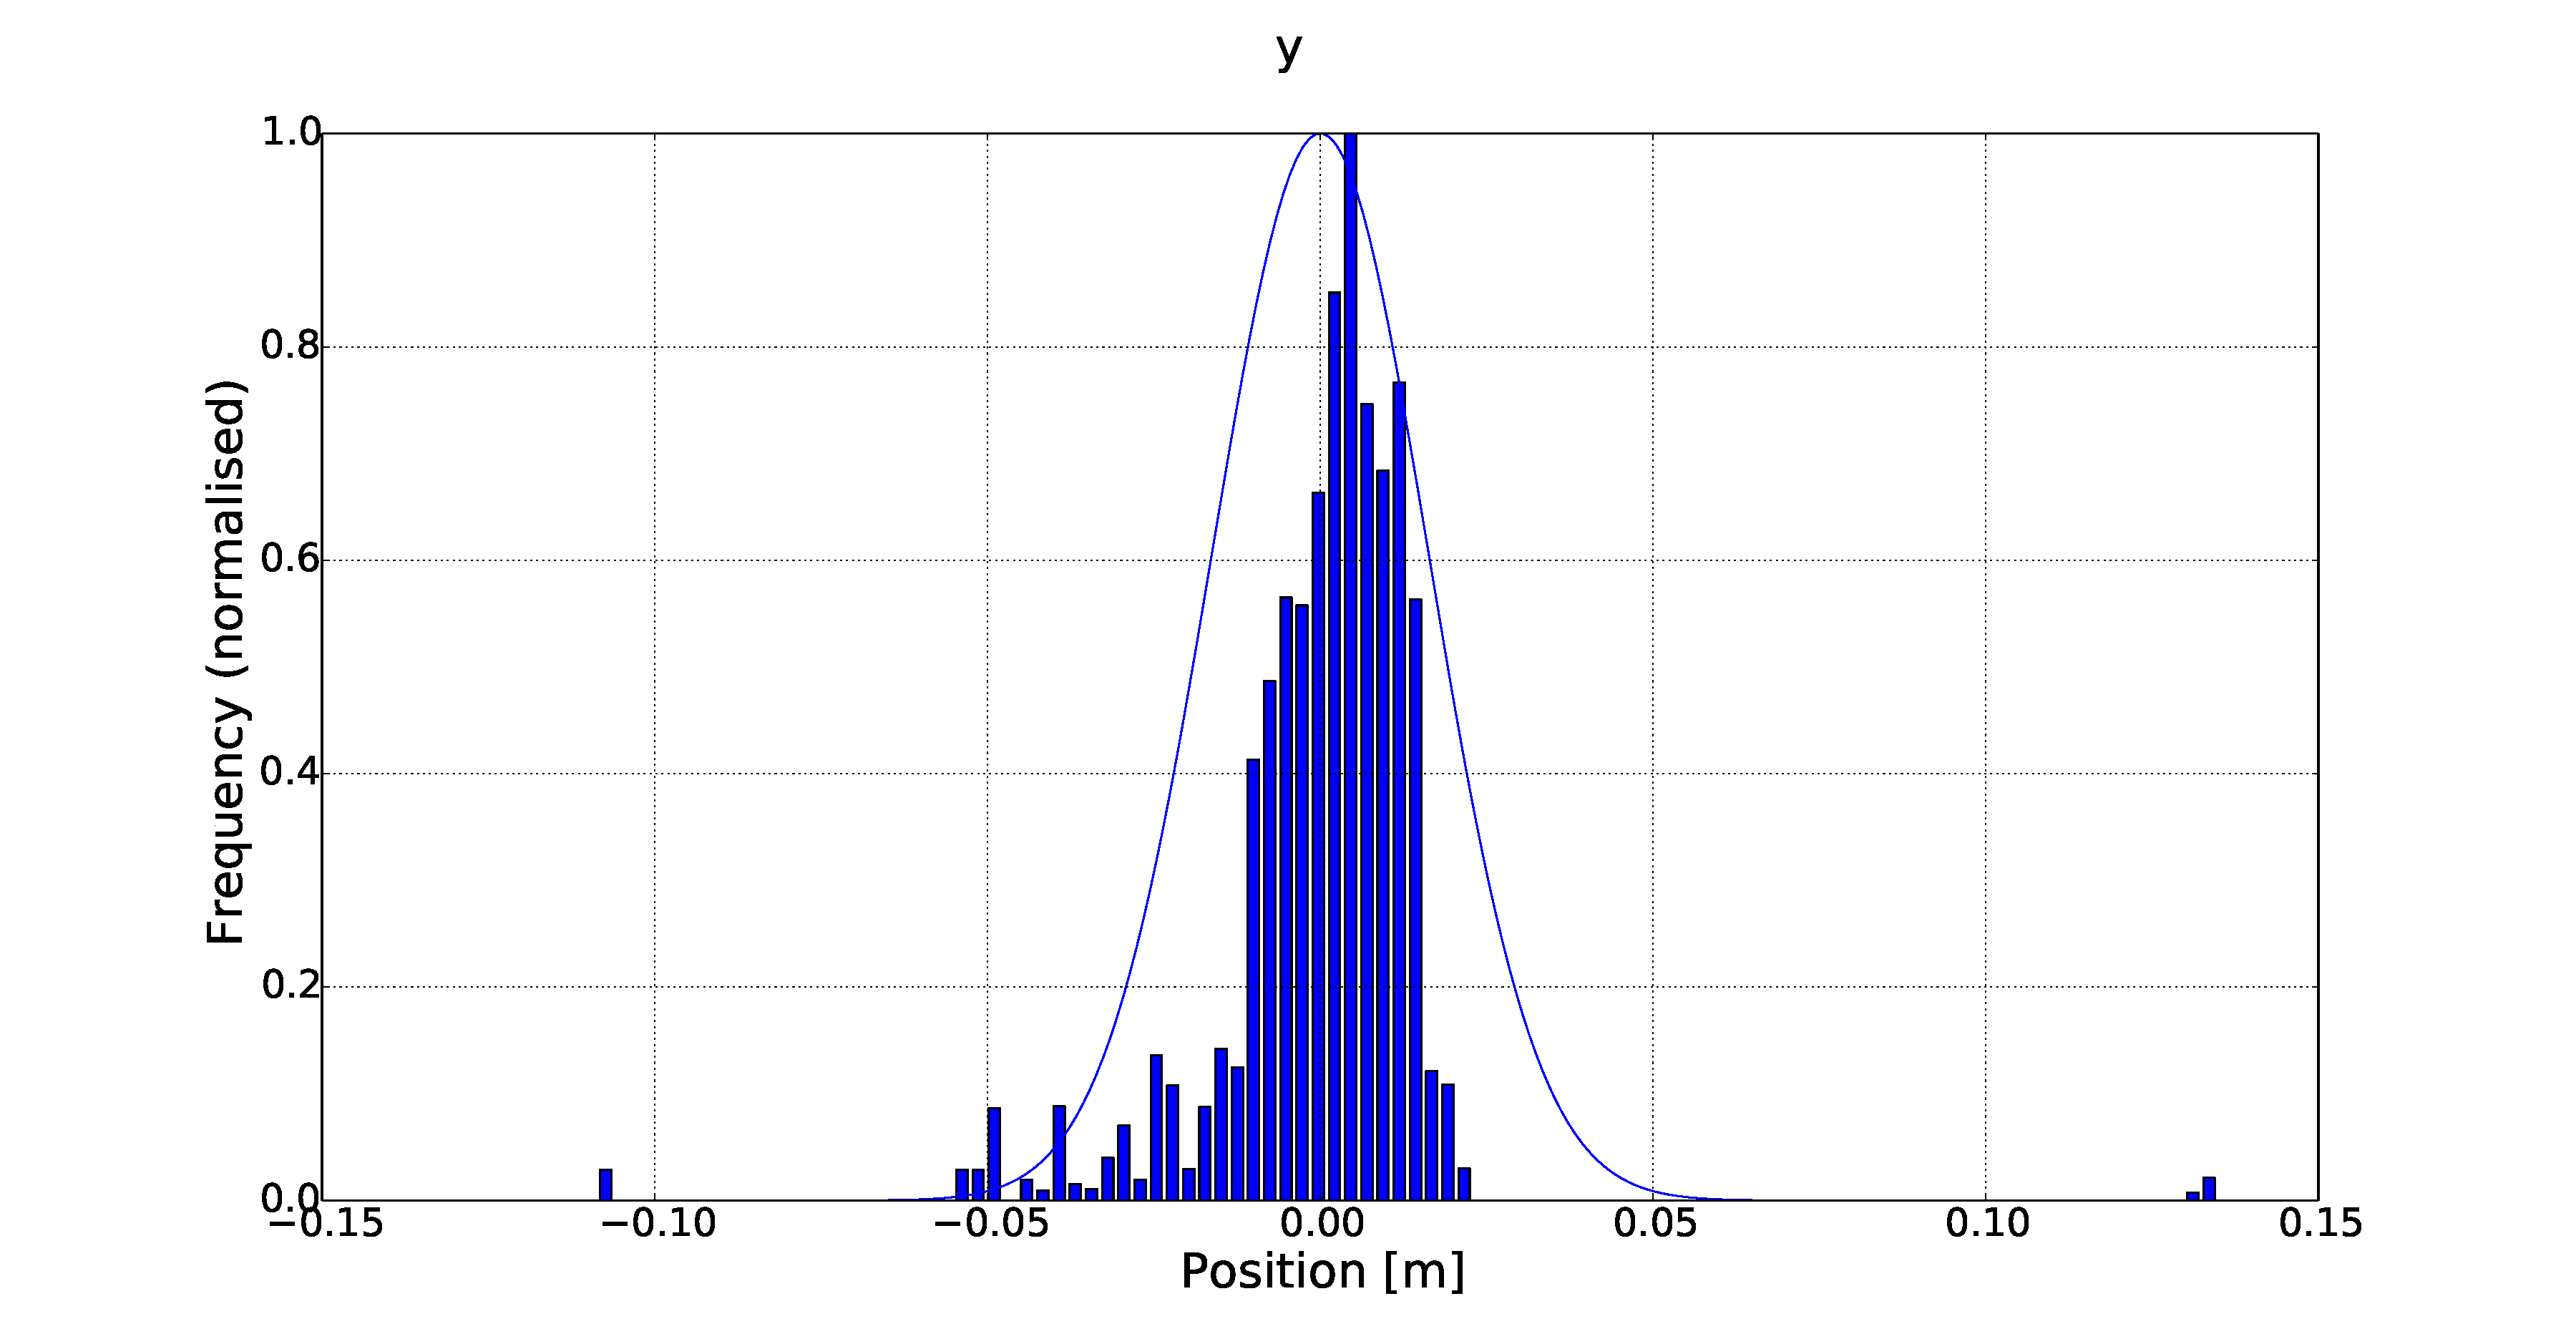
\includegraphics[width=\textwidth]{figures/chapter3/norm_y}
     \caption{Histogram of the error in the $y$ dimension with a mean of $-20.2\mu$m and a standard deviation of 167mm.}
  \label{fig:norm-y}
  \end{subfigure}
~
  \begin{subfigure}{0.45\textwidth}
     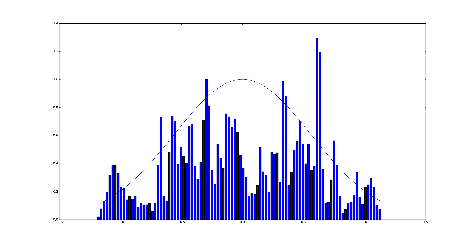
\includegraphics[width=\textwidth]{figures/chapter3/norm_z.pdf}
     \caption{Histogram of the error in the $z$ dimension with a mean of 1.17mm and a standard deviation of 560mm.}
  \label{fig:norm-z}
  \end{subfigure}
~
  \begin{subfigure}{0.45\textwidth}
     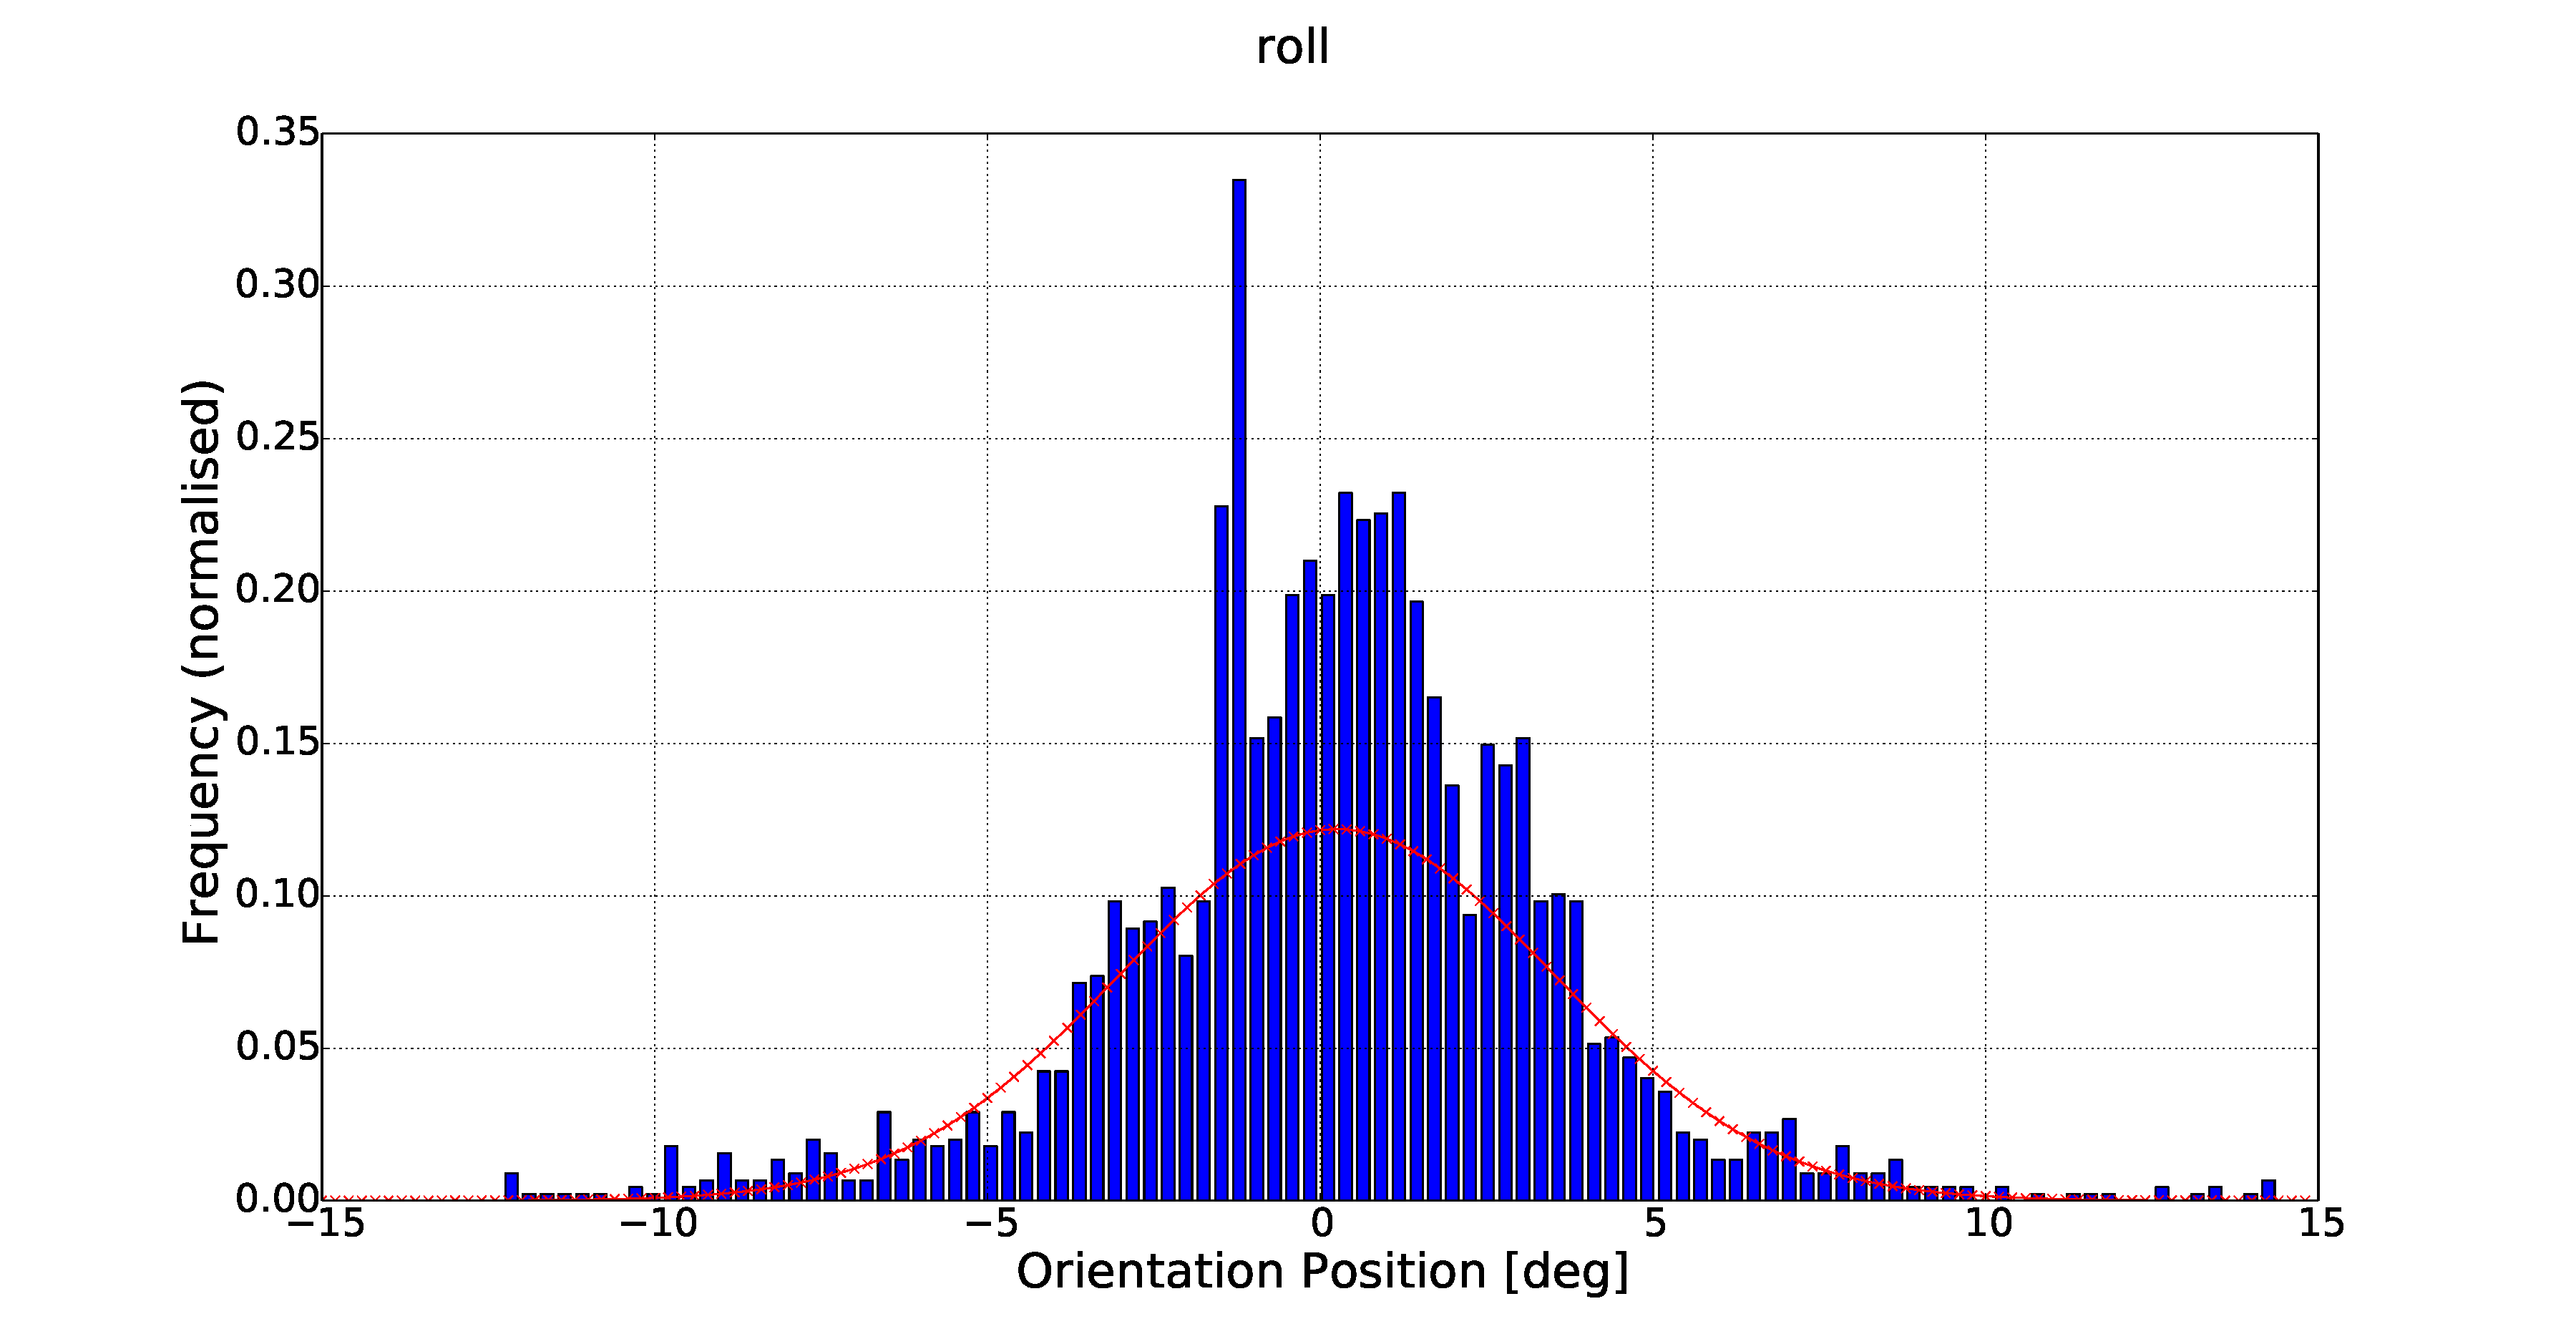
\includegraphics[width=\textwidth]{figures/chapter3/norm_roll.pdf}
     \caption{Histogram of the error in the $\theta$ dimension with a mean of 4 mili-degrees and a standard deviation of 44.0\degree.}
  \label{fig:norm-roll}
  \end{subfigure}
~
  \begin{subfigure}{0.45\textwidth}
     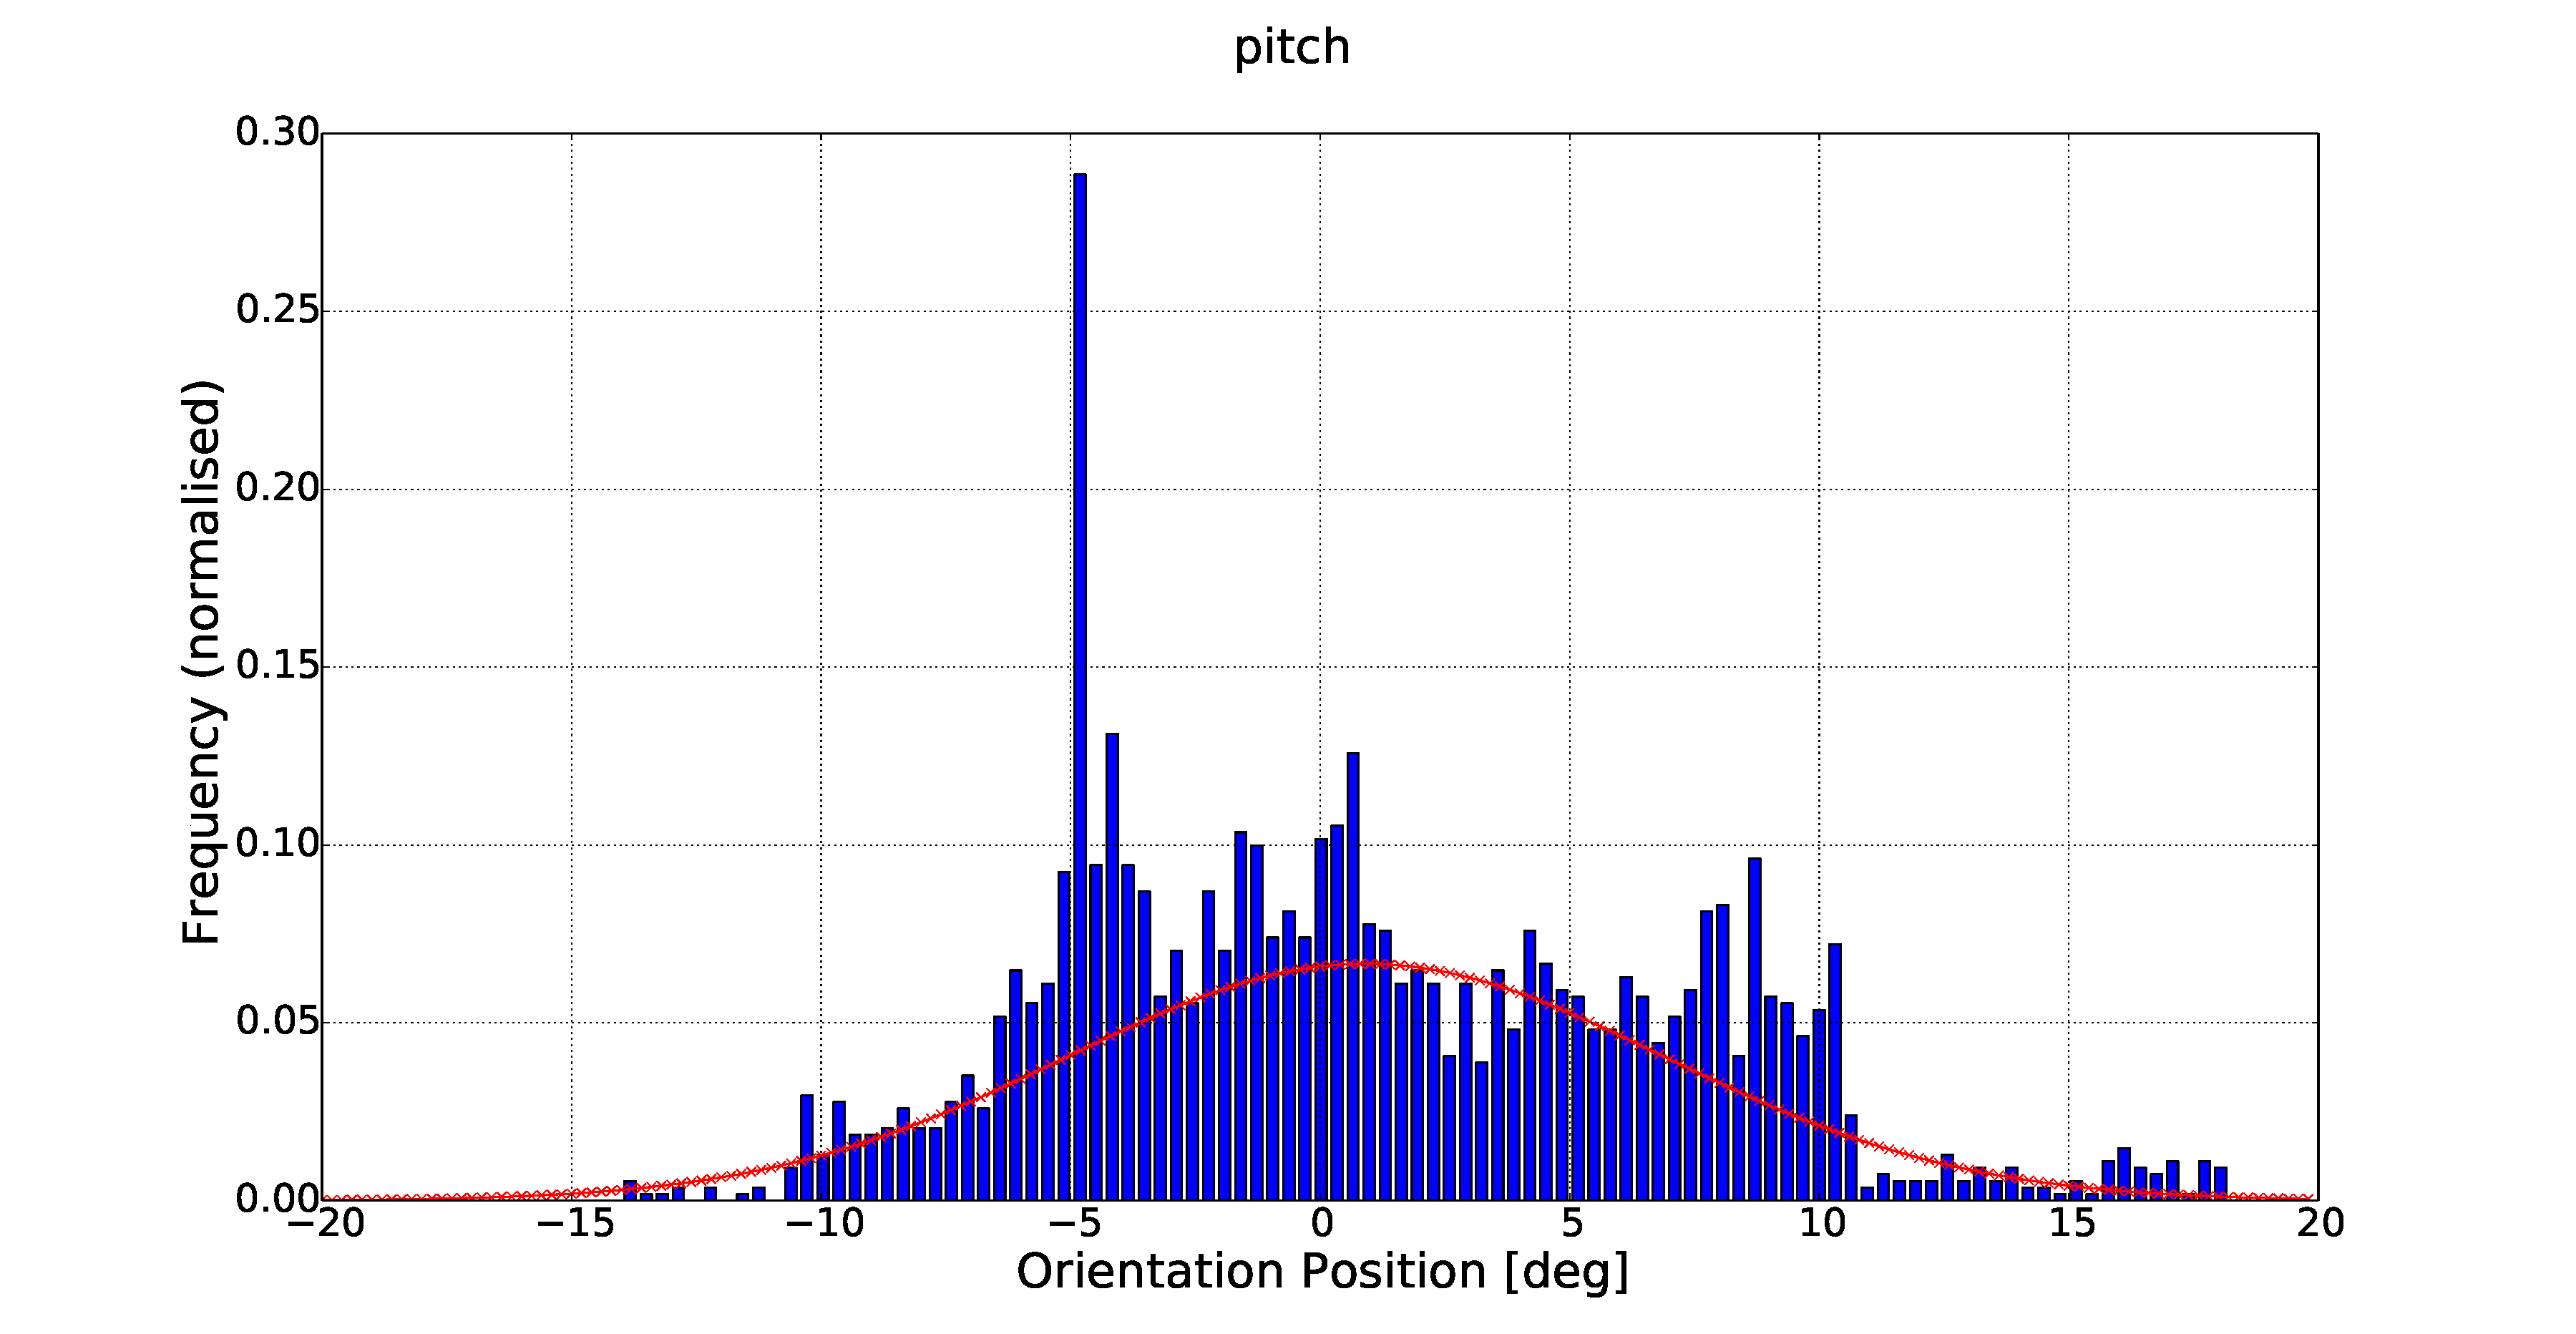
\includegraphics[width=\textwidth]{figures/chapter3/norm_pitch.pdf}
     \caption{Histogram of the error in the $\phi$ dimension with a mean of meme and a standard deviation of meme.}
  \label{fig:norm-pitch}
  \end{subfigure}
~
  \begin{subfigure}{0.45\textwidth}
     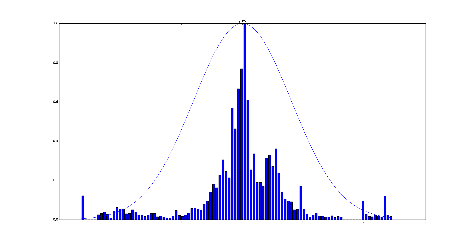
\includegraphics[width=\textwidth]{figures/chapter3/norm_yaw.pdf}
     \caption{Histogram of the error in the $\psi$ dimension with a mean of meme and a standard deviation of meme. }
  \label{fig:norm-yaw}
  \end{subfigure}
  \caption[Plots of the frequency histograms of the error data in each dimension.]{Plots of the frequency histograms of the error data in each dimension.}
  \label{fig:err-norm}
\end{figure*}

It can be seen that all the plots are roughly centred around zero and are very nearly normally distributed. The $z$ dimension displays the largest standard deviation of approximately 560mm. The reason behind this is the bad depth estimates that a single camera system provides. The standard deviations of the other dimensions are within the range that was expected of the system. However, at first glance, the CVS's does not seem to be as accurate as hoped. 

In all, the frequency histogram and normal distribution plots of the errors in Figure~\ref{fig:err-norm} show that the assumption made in Equation~\ref{eq:chap3-eq2-offset}, that the errors are normally distributed around zero, is a valid one. 

\subsection{Optimum Focal Lengths and Offset}

HERSIEN MEME

As a result of the focal length and offset optimisation procedure, the optimal focal lengths, $f_x$ and $f_y$ were found to be 628 and 535 after 50 iterations of the algorithm, which is considerably less than the optimum of 700 produced by OpenCV's calibration toolbox. Note that these units are given in camera pixel units and not millimetres.

The optimal offset $\bar{\bm{P}}$ was found and is given in Equation~\ref{eq:chap3-offset-value}.

\begin{equation}
  \label{eq:chap3-offset-value}
  \bar{\bm{P}} = 
  \begin{bmatrix}
    240.8mm & 40.09mm & 375.9mm & \ang{184.3} & \ang{-2.697} & \ang{-179.9}
  \end{bmatrix}^T
\end{equation}

The values in $\bar{\bm{P}}$ contain any constant error bias, as well as marker placement errors that may have been introduced to the Vicon test during the measurement process. The large offsets of $\pm\ang{180}$ in the $\theta$ and $\psi$ dimensions can be explained by the differing axis orientations of the CVS camera and Vicon systems, where the axes needed rotating to coincide with one another. This indicates that the offset was correctly calculated and is working as expected. The large offset in the $z$ dimension is to be expected, since single camera's are known to produce very bad depth estimates. However, the relatively large offset of 240mm in the $x$ dimension is slightly surprising, but may be explained if the CVS's camera was placed approximately 240mm from the Vicon system's origin. 

All of the above produce an error two-norm of approximately 0.81 (normalised), compared to the original 1.15 (normalised), showing an overall reduction in the error vector magnitude. Figure~\ref{fig:estimate} shows the results of the Vicon measurements compared to the original and improved CVS measurements in all six dimensions.

\begin{figure*}
  \begin{subfigure}{0.45\textwidth}
    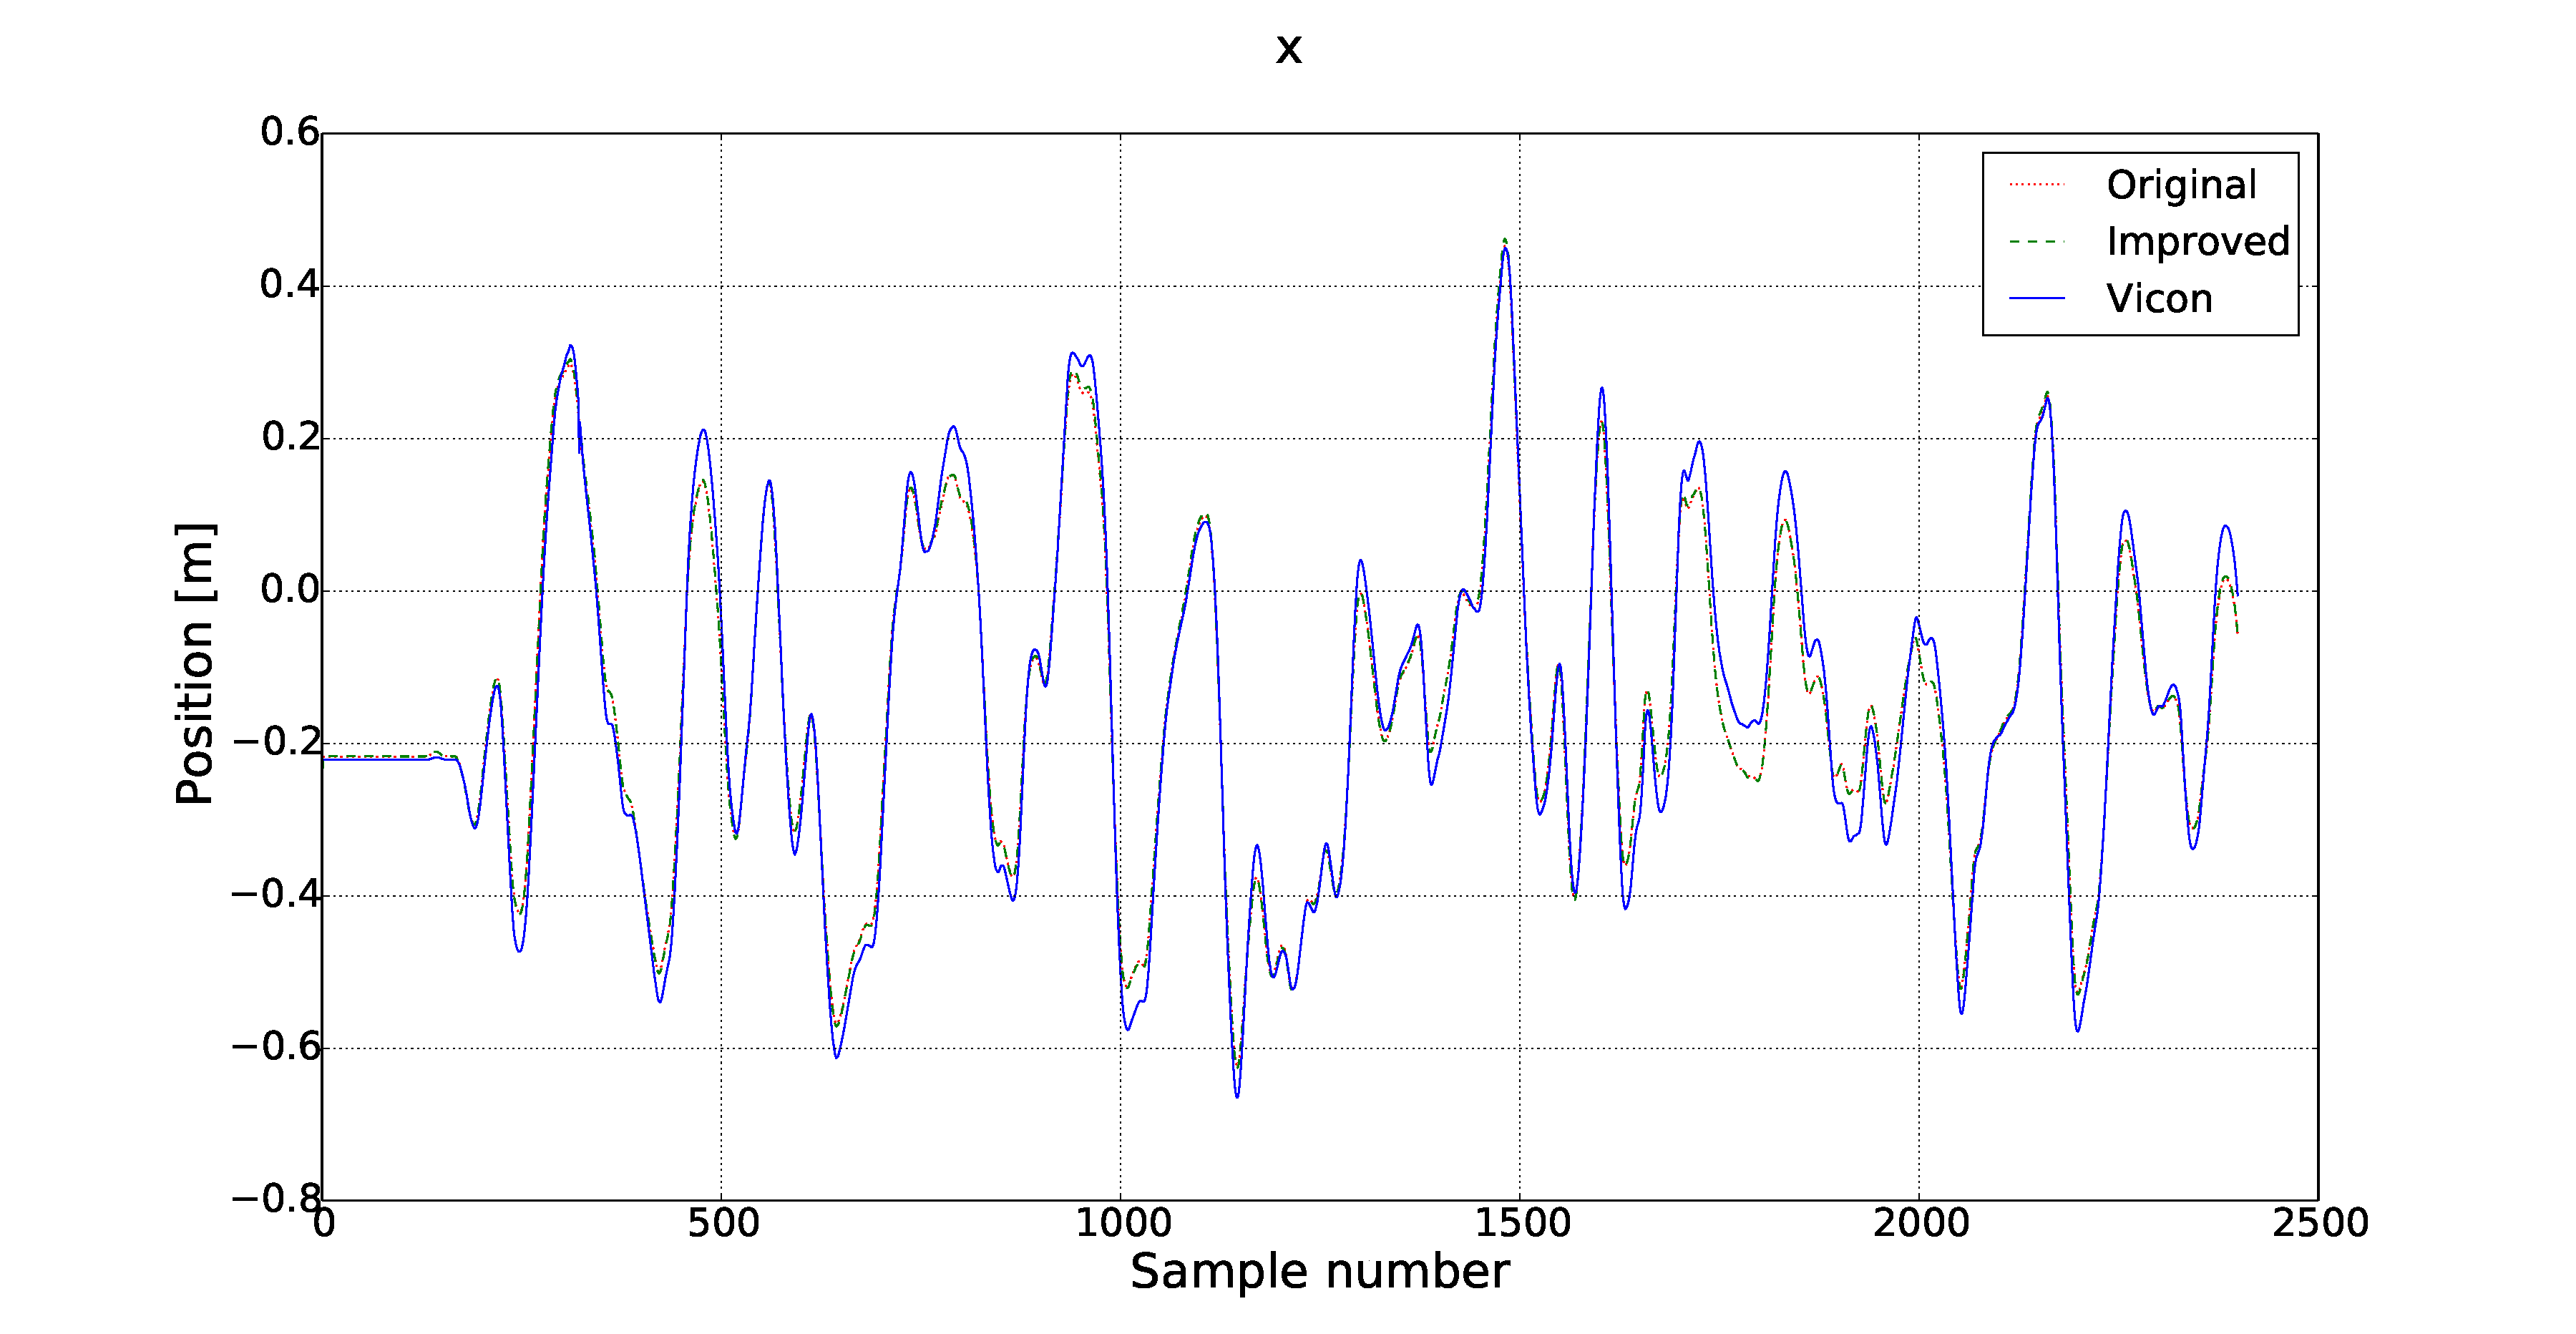
\includegraphics[width=\textwidth]{figures/chapter3/x}
    \caption{The ground-truth Vicon pose estimate, versus the original and improved CV pose estimates in the $x$ dimension.}
  \label{fig:estimate-x}
  \end{subfigure}
~
  \begin{subfigure}{0.45\textwidth}
    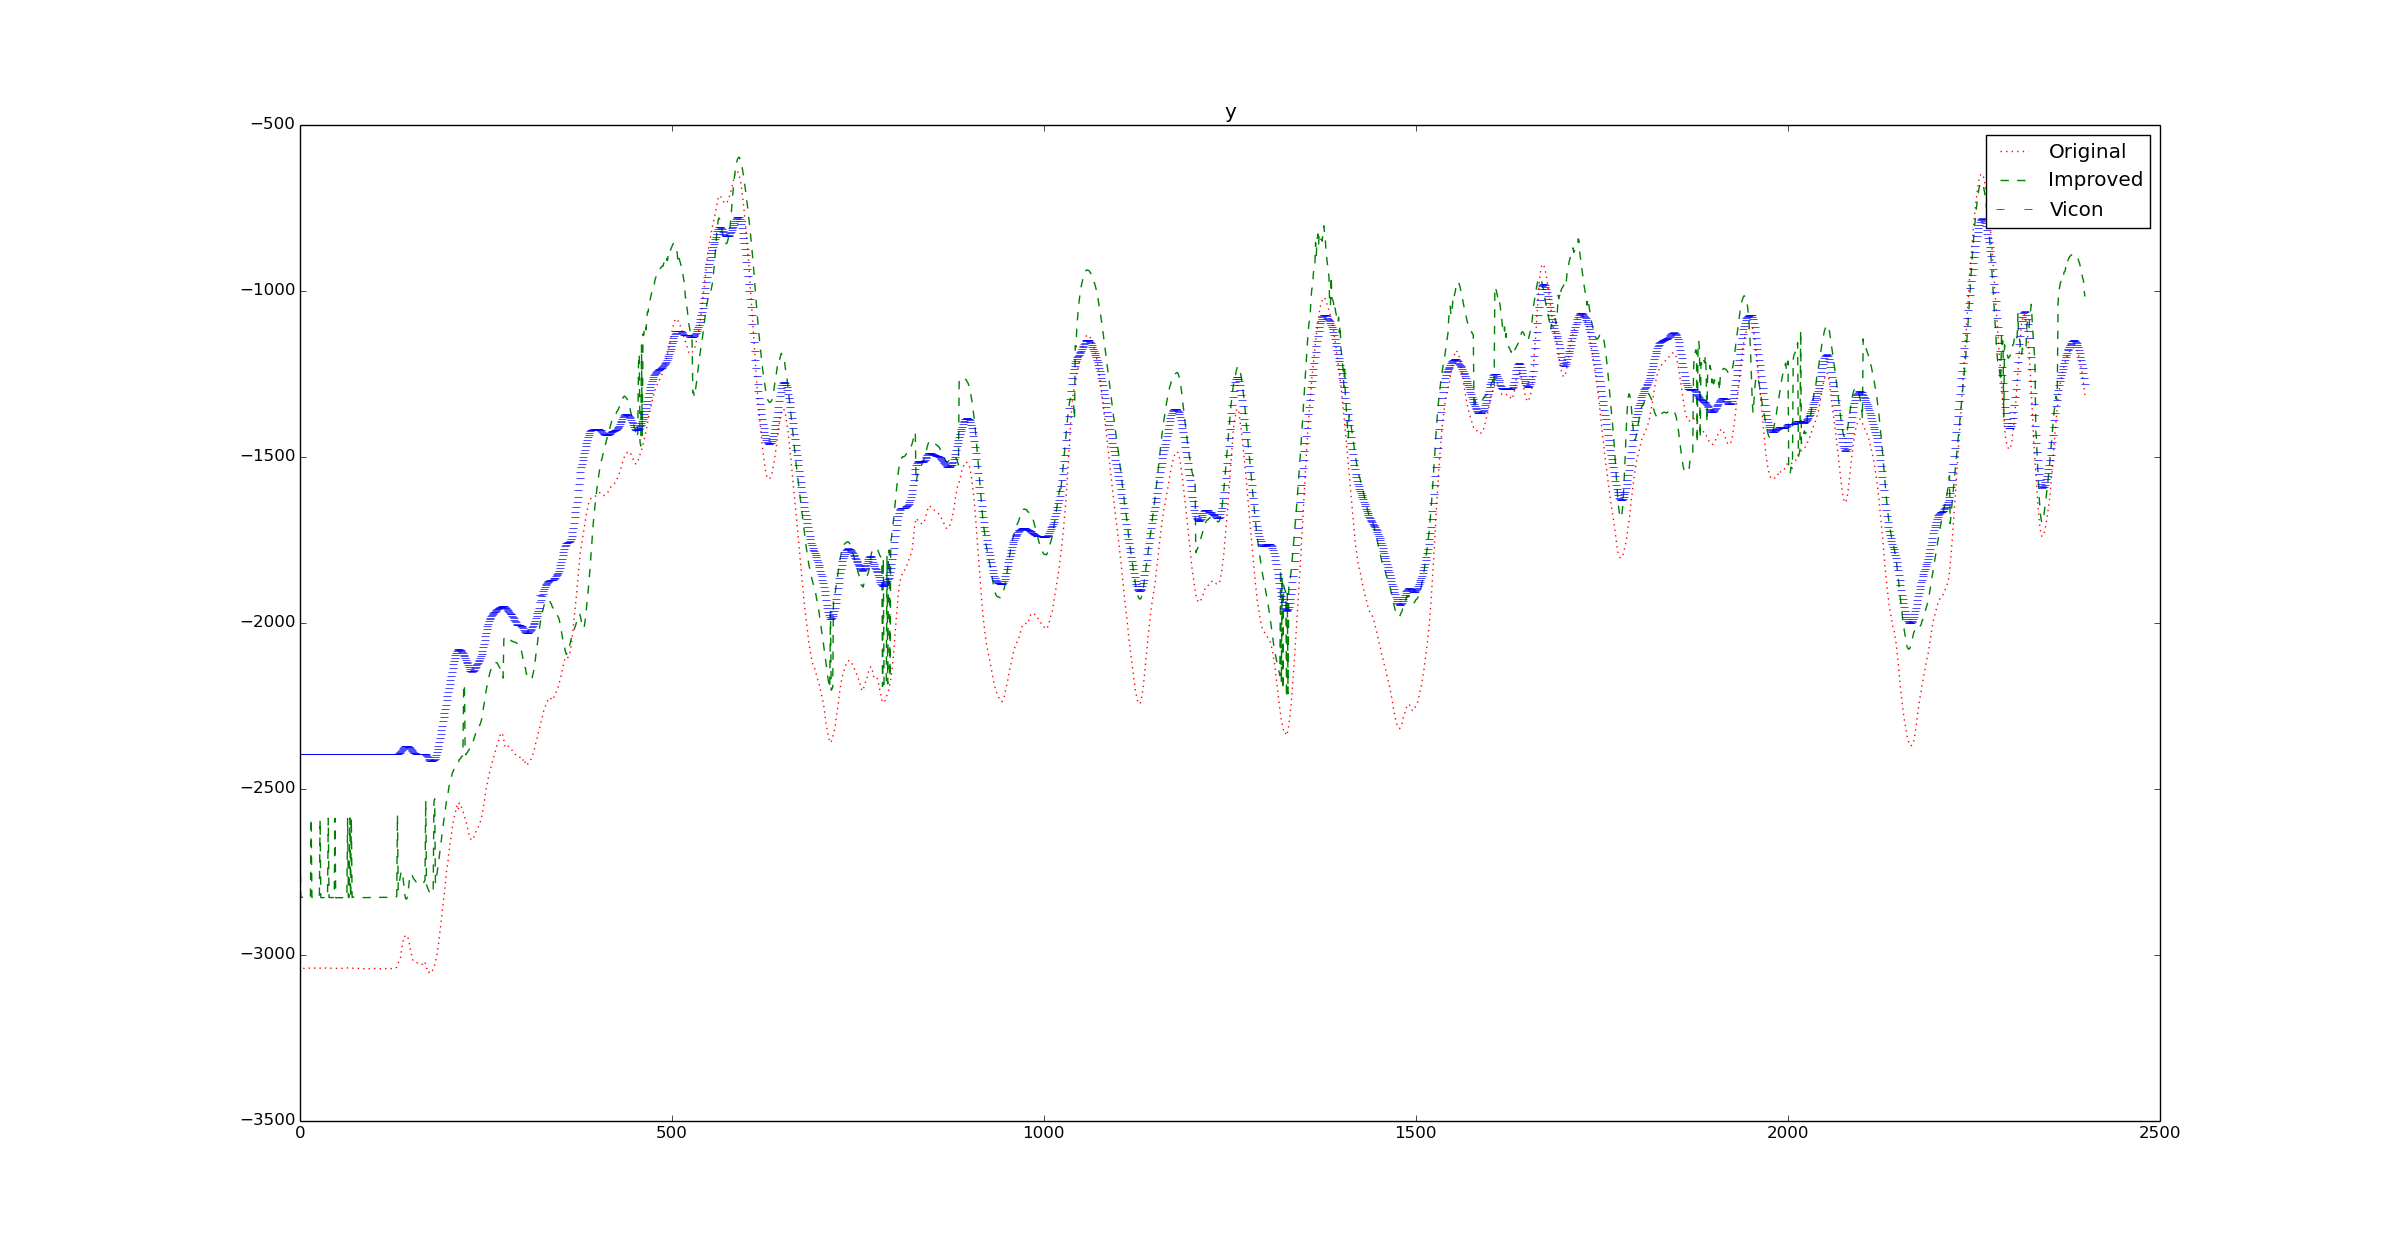
\includegraphics[width=\textwidth]{figures/chapter3/y}
    \caption{The ground-truth Vicon pose estimate, versus the original and improved CV pose estimates in the $y$ dimension.}
  \label{fig:estimate-y}
  \end{subfigure}
~
  \begin{subfigure}{0.45\textwidth}
    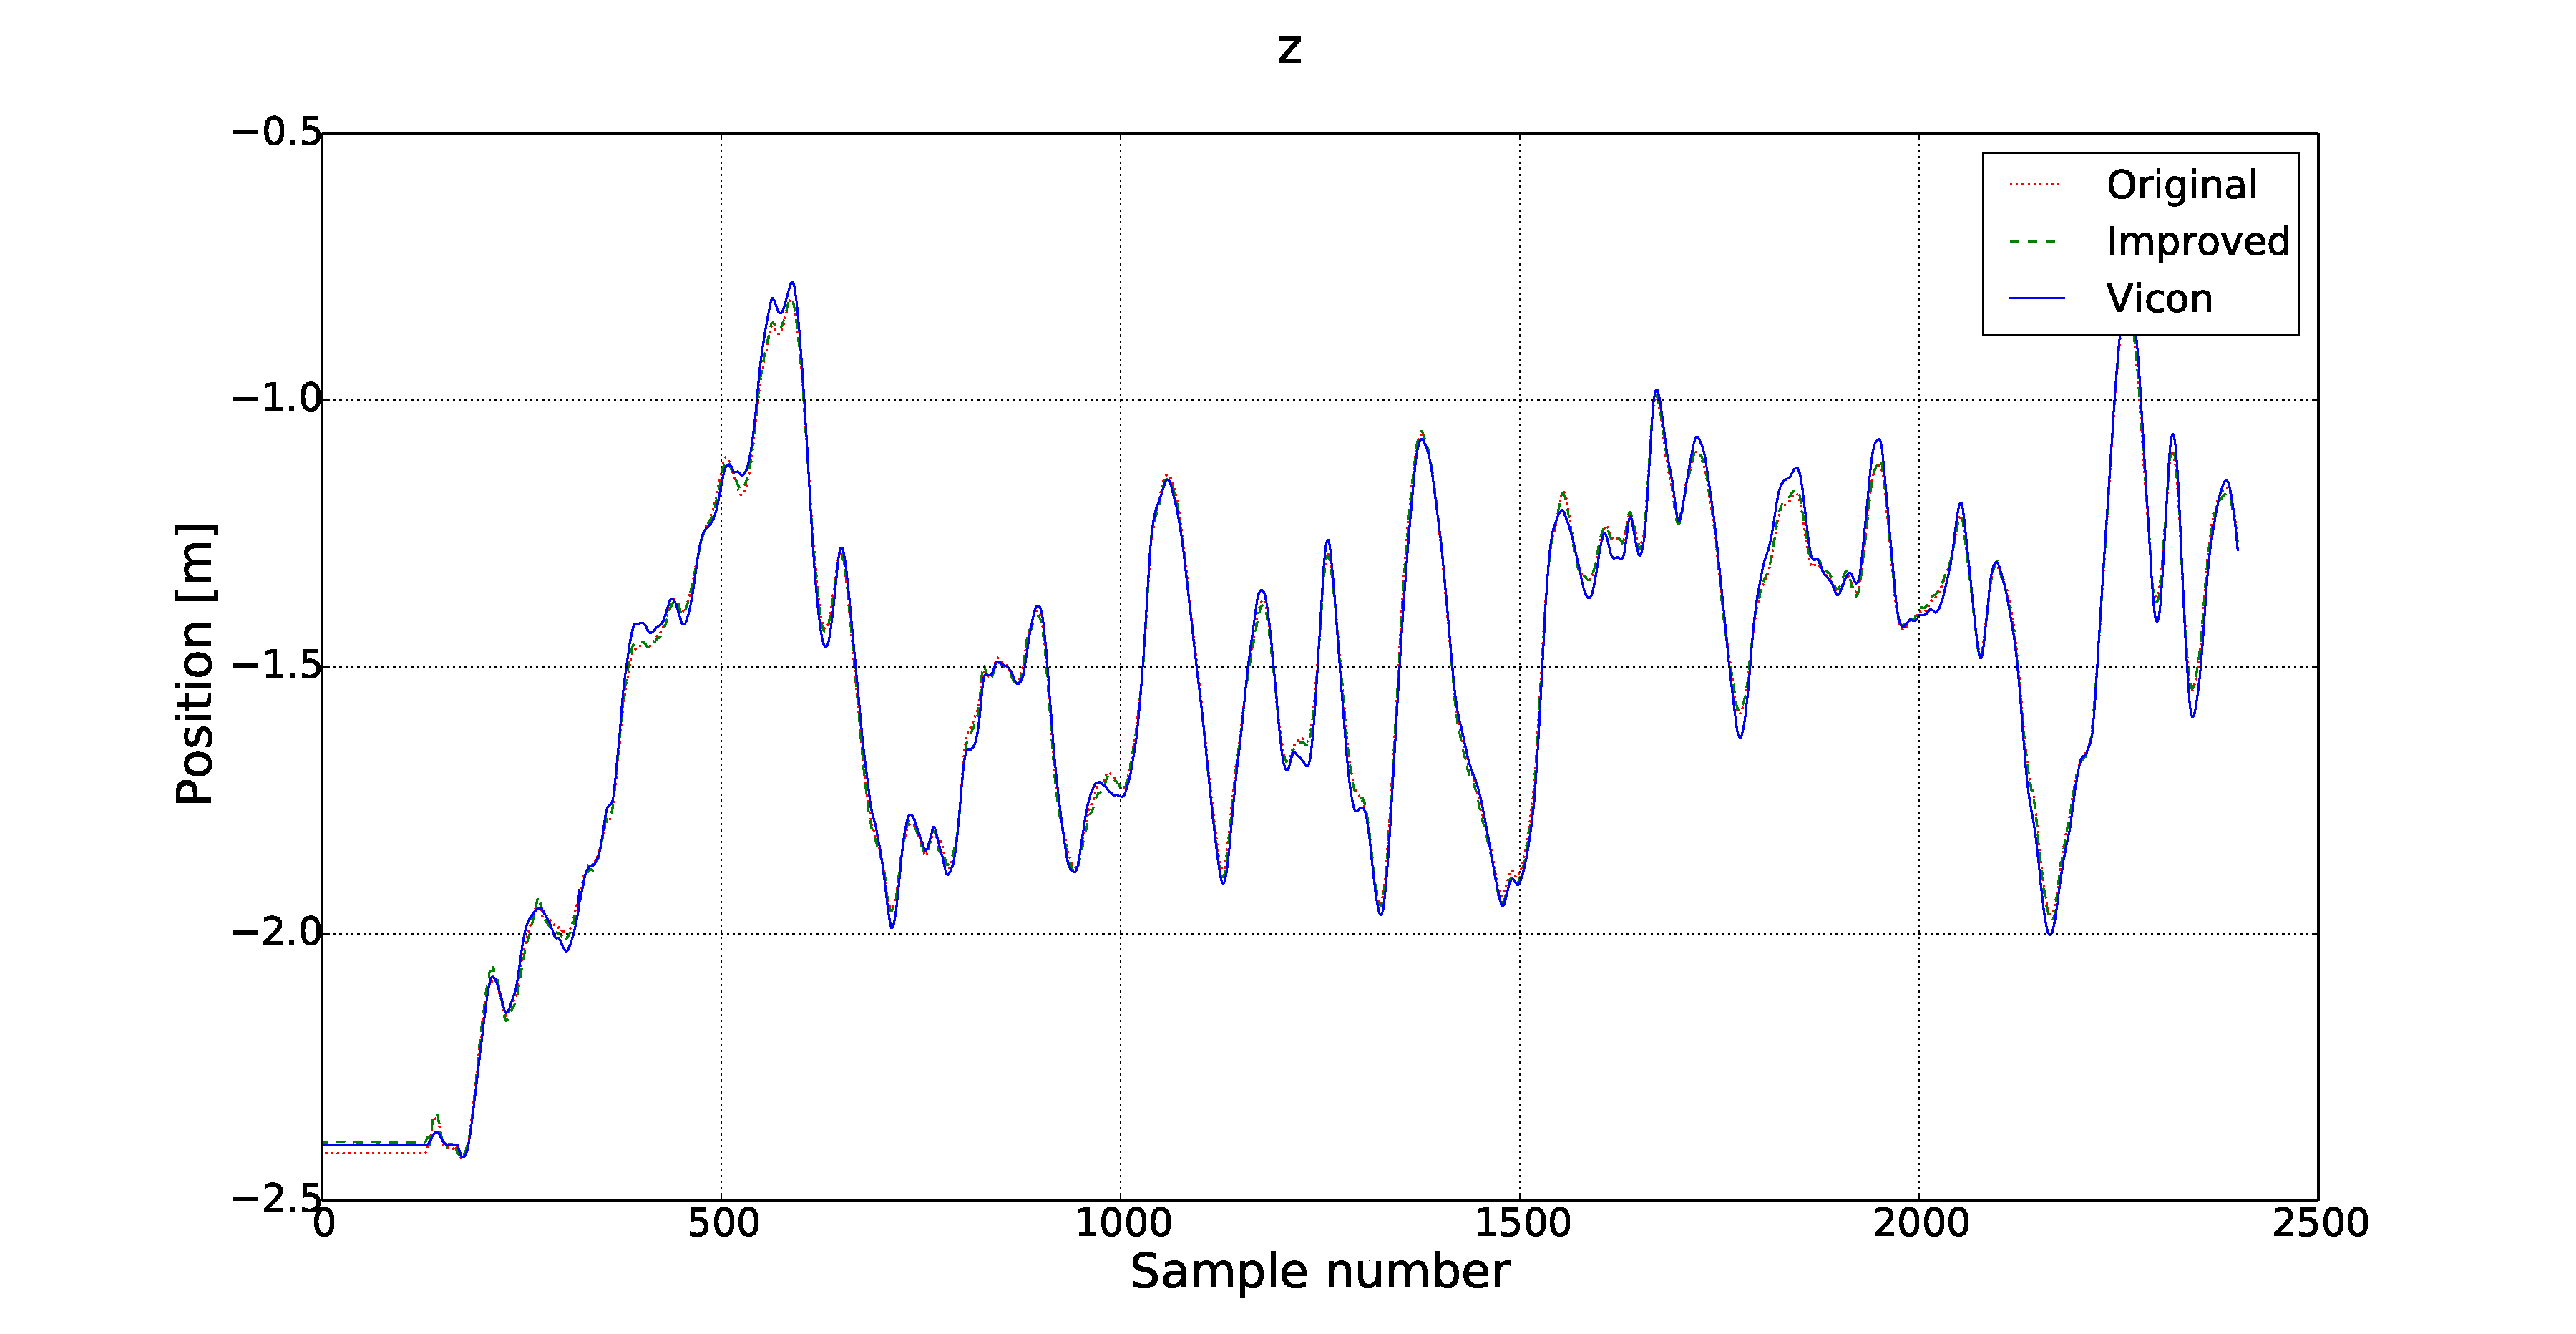
\includegraphics[width=\textwidth]{figures/chapter3/z}
    \caption{The ground-truth Vicon pose estimate, versus the original and improved CV pose estimates in the $z$ dimension.}
  \label{fig:estimate-z}
  \end{subfigure}
~
  \begin{subfigure}{0.45\textwidth}
    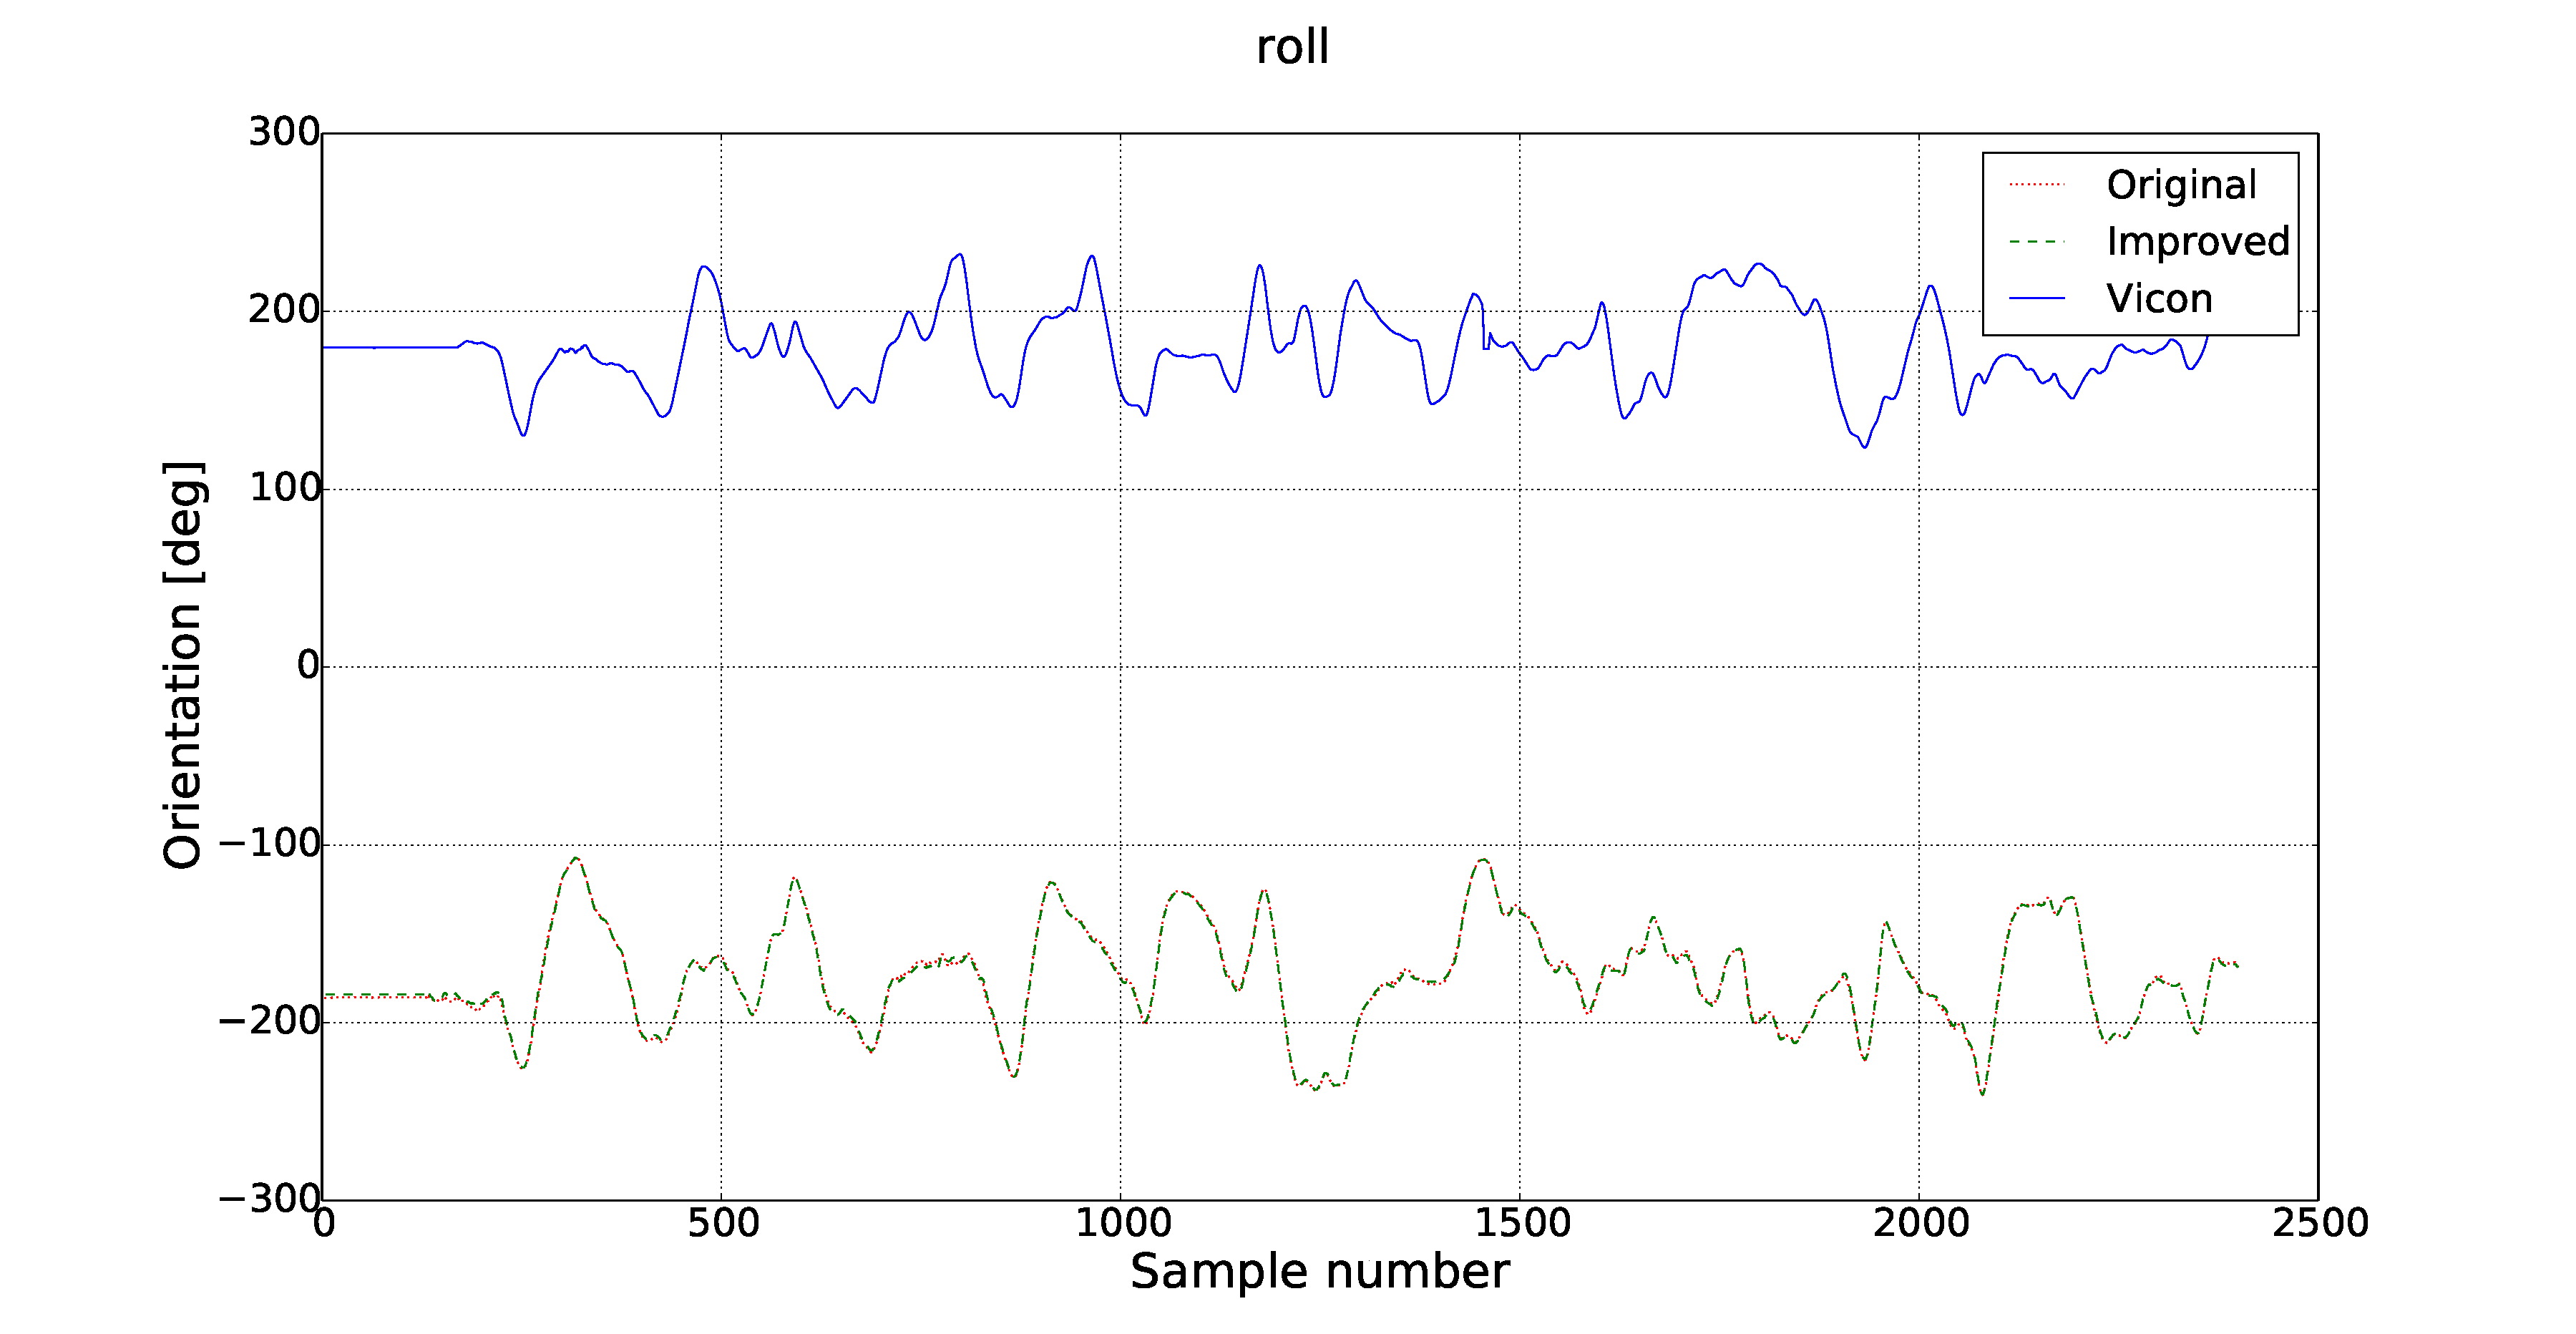
\includegraphics[width=\textwidth]{figures/chapter3/roll}
    \caption{The ground-truth Vicon pose estimate, versus the original and improved CV pose estimates in the $\theta$ dimension.}
  \label{fig:estimate-roll}
  \end{subfigure}
~
  \begin{subfigure}{0.45\textwidth}
    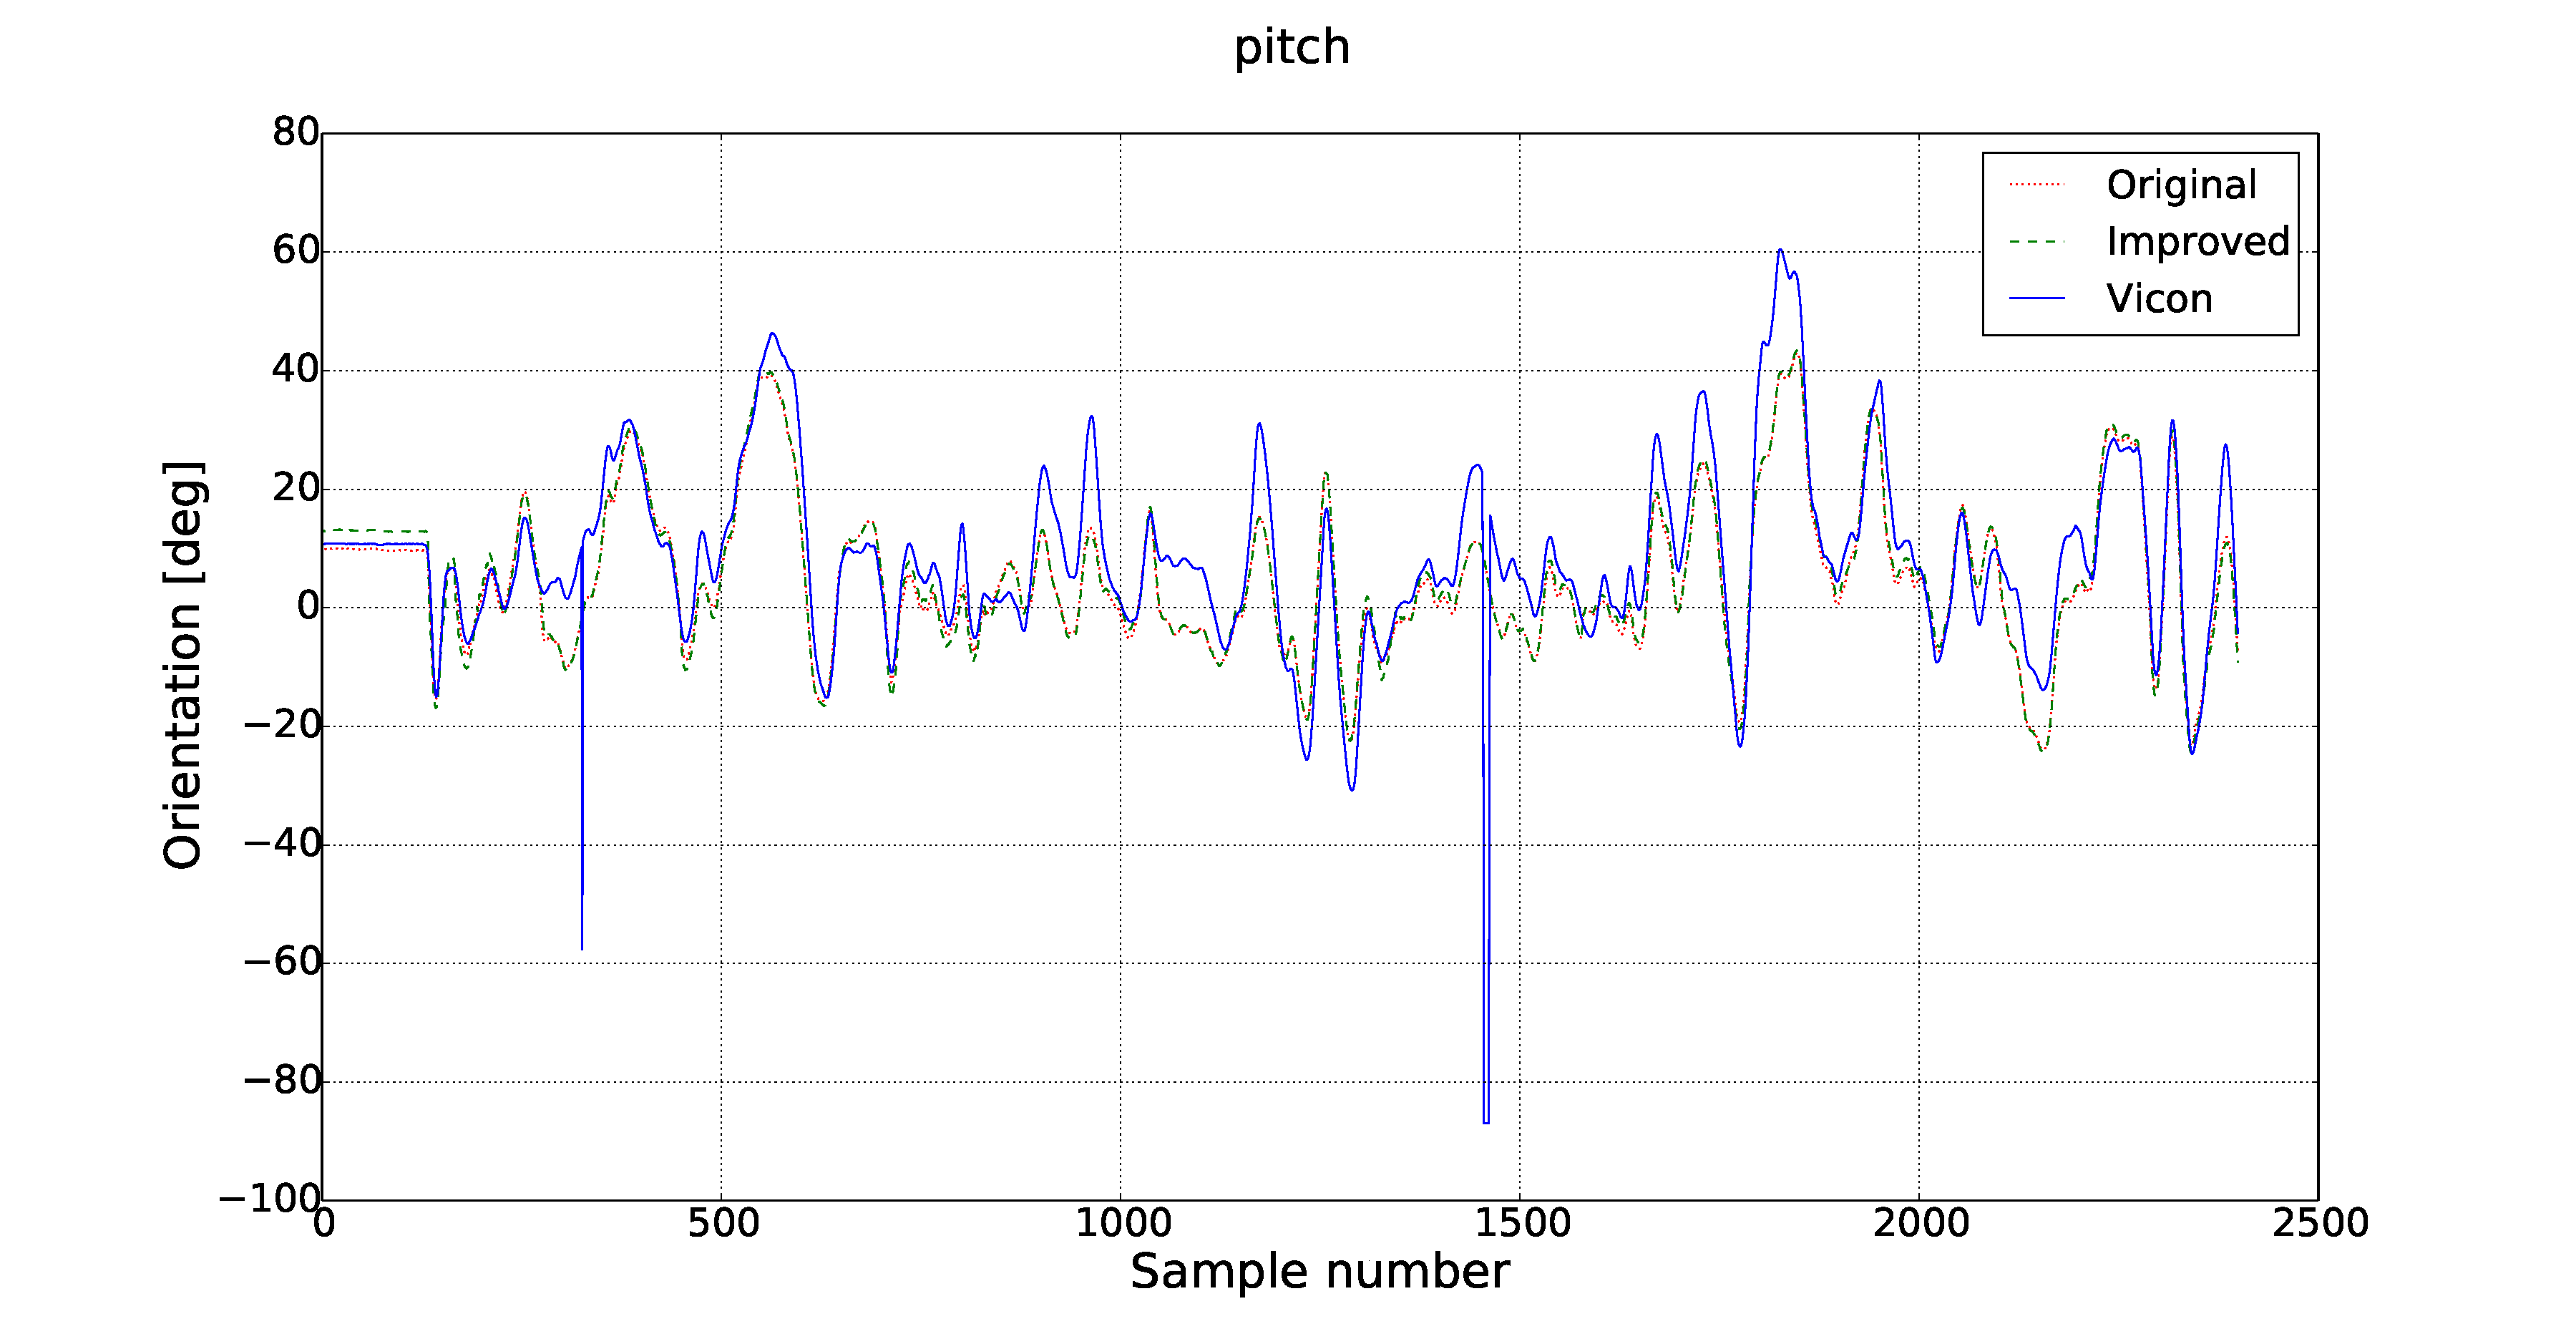
\includegraphics[width=\textwidth]{figures/chapter3/pitch}
    \caption{The ground-truth Vicon pose estimate, versus the original and improved CV pose estimates in the $\phi$ dimension.}
  \label{fig:estimate-pitch}
  \end{subfigure}
~
  \begin{subfigure}{0.45\textwidth}
    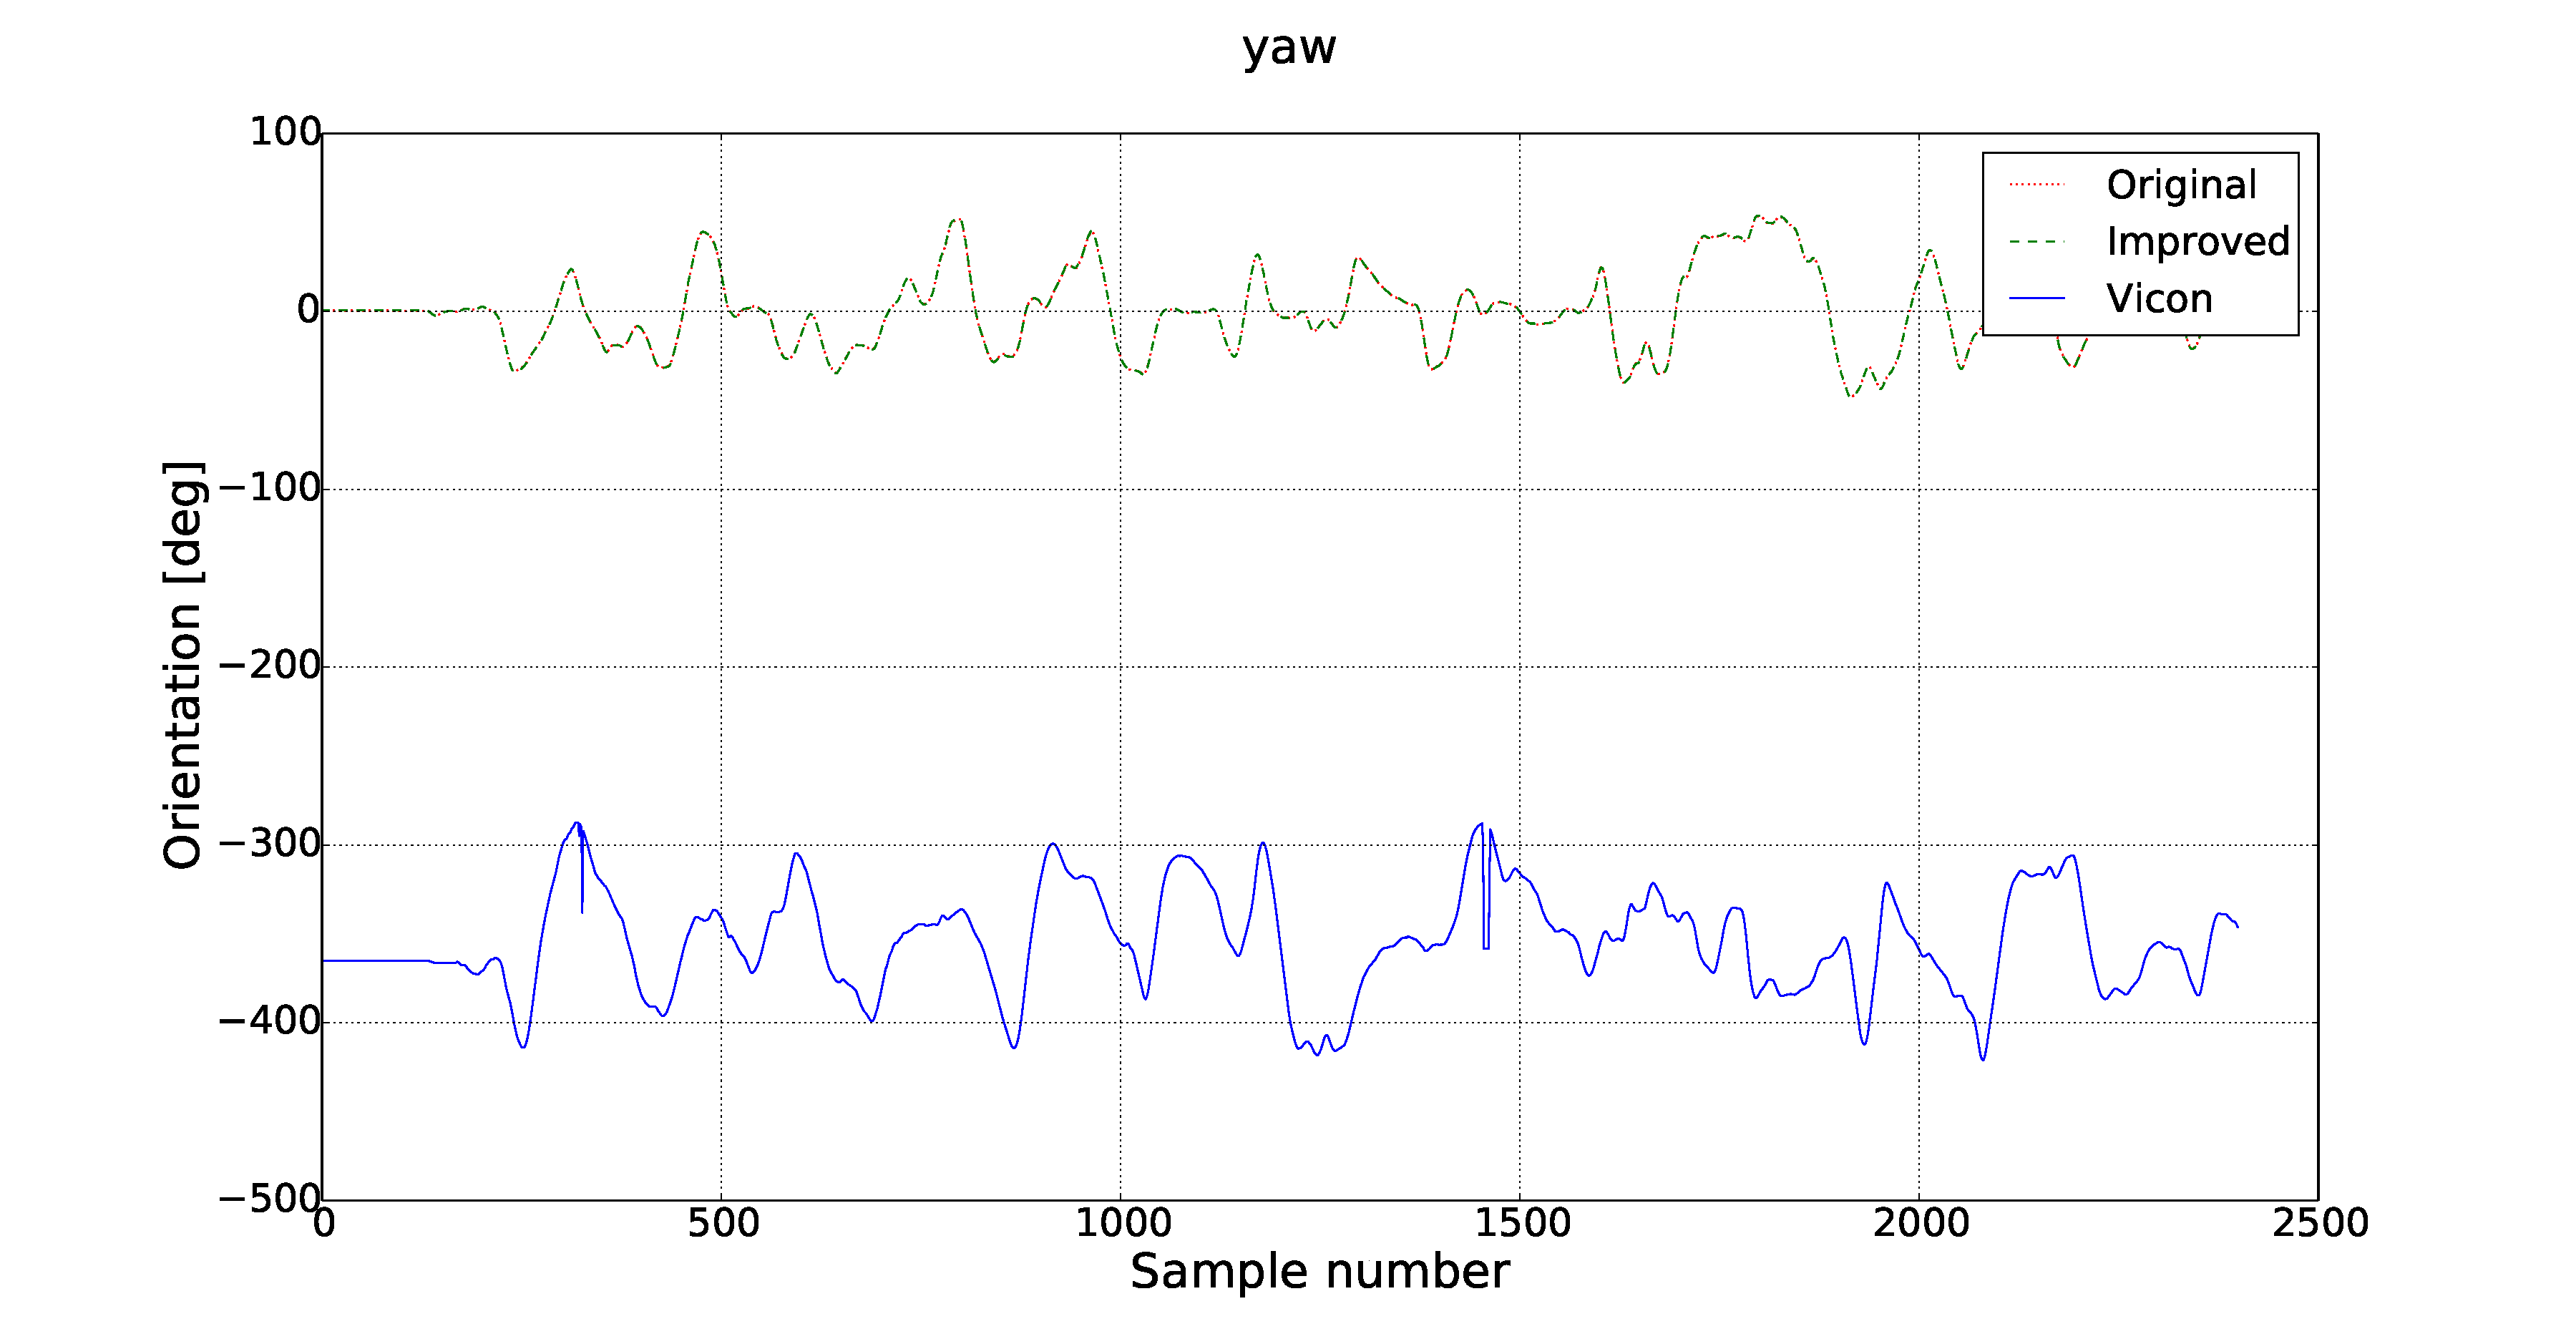
\includegraphics[width=\textwidth]{figures/chapter3/yaw}
    \caption{The ground-truth Vicon pose estimate, versus the original and improved CV pose estimates in the $\psi$ dimension.}
  \label{fig:estimate-yaw}
  \end{subfigure}
  \caption[Plots comparing the Vicon's measurements with the CVS's original and improved measurements. ]{Plots comparing the Vicon's pose measurements with the CVS's original estimate, as well as the estimate with the optimal focal length combination.}
  \label{fig:estimate}
\end{figure*}

It can be seen that there is some improvement in all the dimensions. However, in some cases the improvement in one section of the data set, is negated by worse estimates in another. This can be attributed to the optimisation process, where an improvement at timeframe $t_i$ in the $x$ dimension, for example, may lead to a worse estimate at time $t_i$ in the $\phi$ dimension. However, as the reduction in the two-norm magnitude of the error proves, there is an overall reduction in the error with the optimised data set. It can therefore be concluded that the optimisation procedure did indeed function as expected, producing a focal length combination which led to a more accurate pose estimate from the CVS. 

\subsection{Computer Vision System Accuracy}

Determining the accuracy of a multi-dimensional data model is often a complex task, but since it was found that the error $\bm{\epsilon}$ is normally distributed about zero, it is possible to use the covariance matrix to check the interdimensional variance and dependence. If the off-diagonal elements of the covariance matrix is sufficiently small enough relative to the diagonal elements, it can be deduced that the dimensions are strong enough independent of one another. The covariance matrix $\bm{\Sigma}$ is given in Equation~\ref{eq:covariance-matrix}. 

\begin{equation}
  \label{eq:covariance-matrix}
  \bm{\Sigma} = 
  \begin{bmatrix}
    \bm{3131.7} & 2255.2 & 98.227 & 94.371 &  98.830 & 106.85 \\ 
    2255.2 & \bm{40924}  & 4038.2 & 197.46 &  30.631 & 1953.7 \\
    98.227 & 4038.2 & \bm{5592.5} & 241.75 &  106.86 & 385.23 \\
    94.371 & 197.46 & 241.75 & \bm{84.939} &  10.303 & 13.792 \\
    98.830 & 30.631 & 106.86 & 10.303 &  \bm{110.54} & 63.381 \\
    106.85 & 1953.7 & 385.23 & 13.792 &  63.381 & \bm{318.17} \\
  \end{bmatrix}
\end{equation}

The matrix $\bm{\Sigma}$ shows that there are large off-diagonal elements, indicating that there is strong interdimensional dependence. This dependence is further demonstrated when examining the change in the error in a dimension with respect to the other dimensions. This is demonstrated in the contour plots of Figure~\ref{fig:err-contour}. 

\begin{figure*}
  \centering
  \begin{subfigure}{0.31\textwidth}
    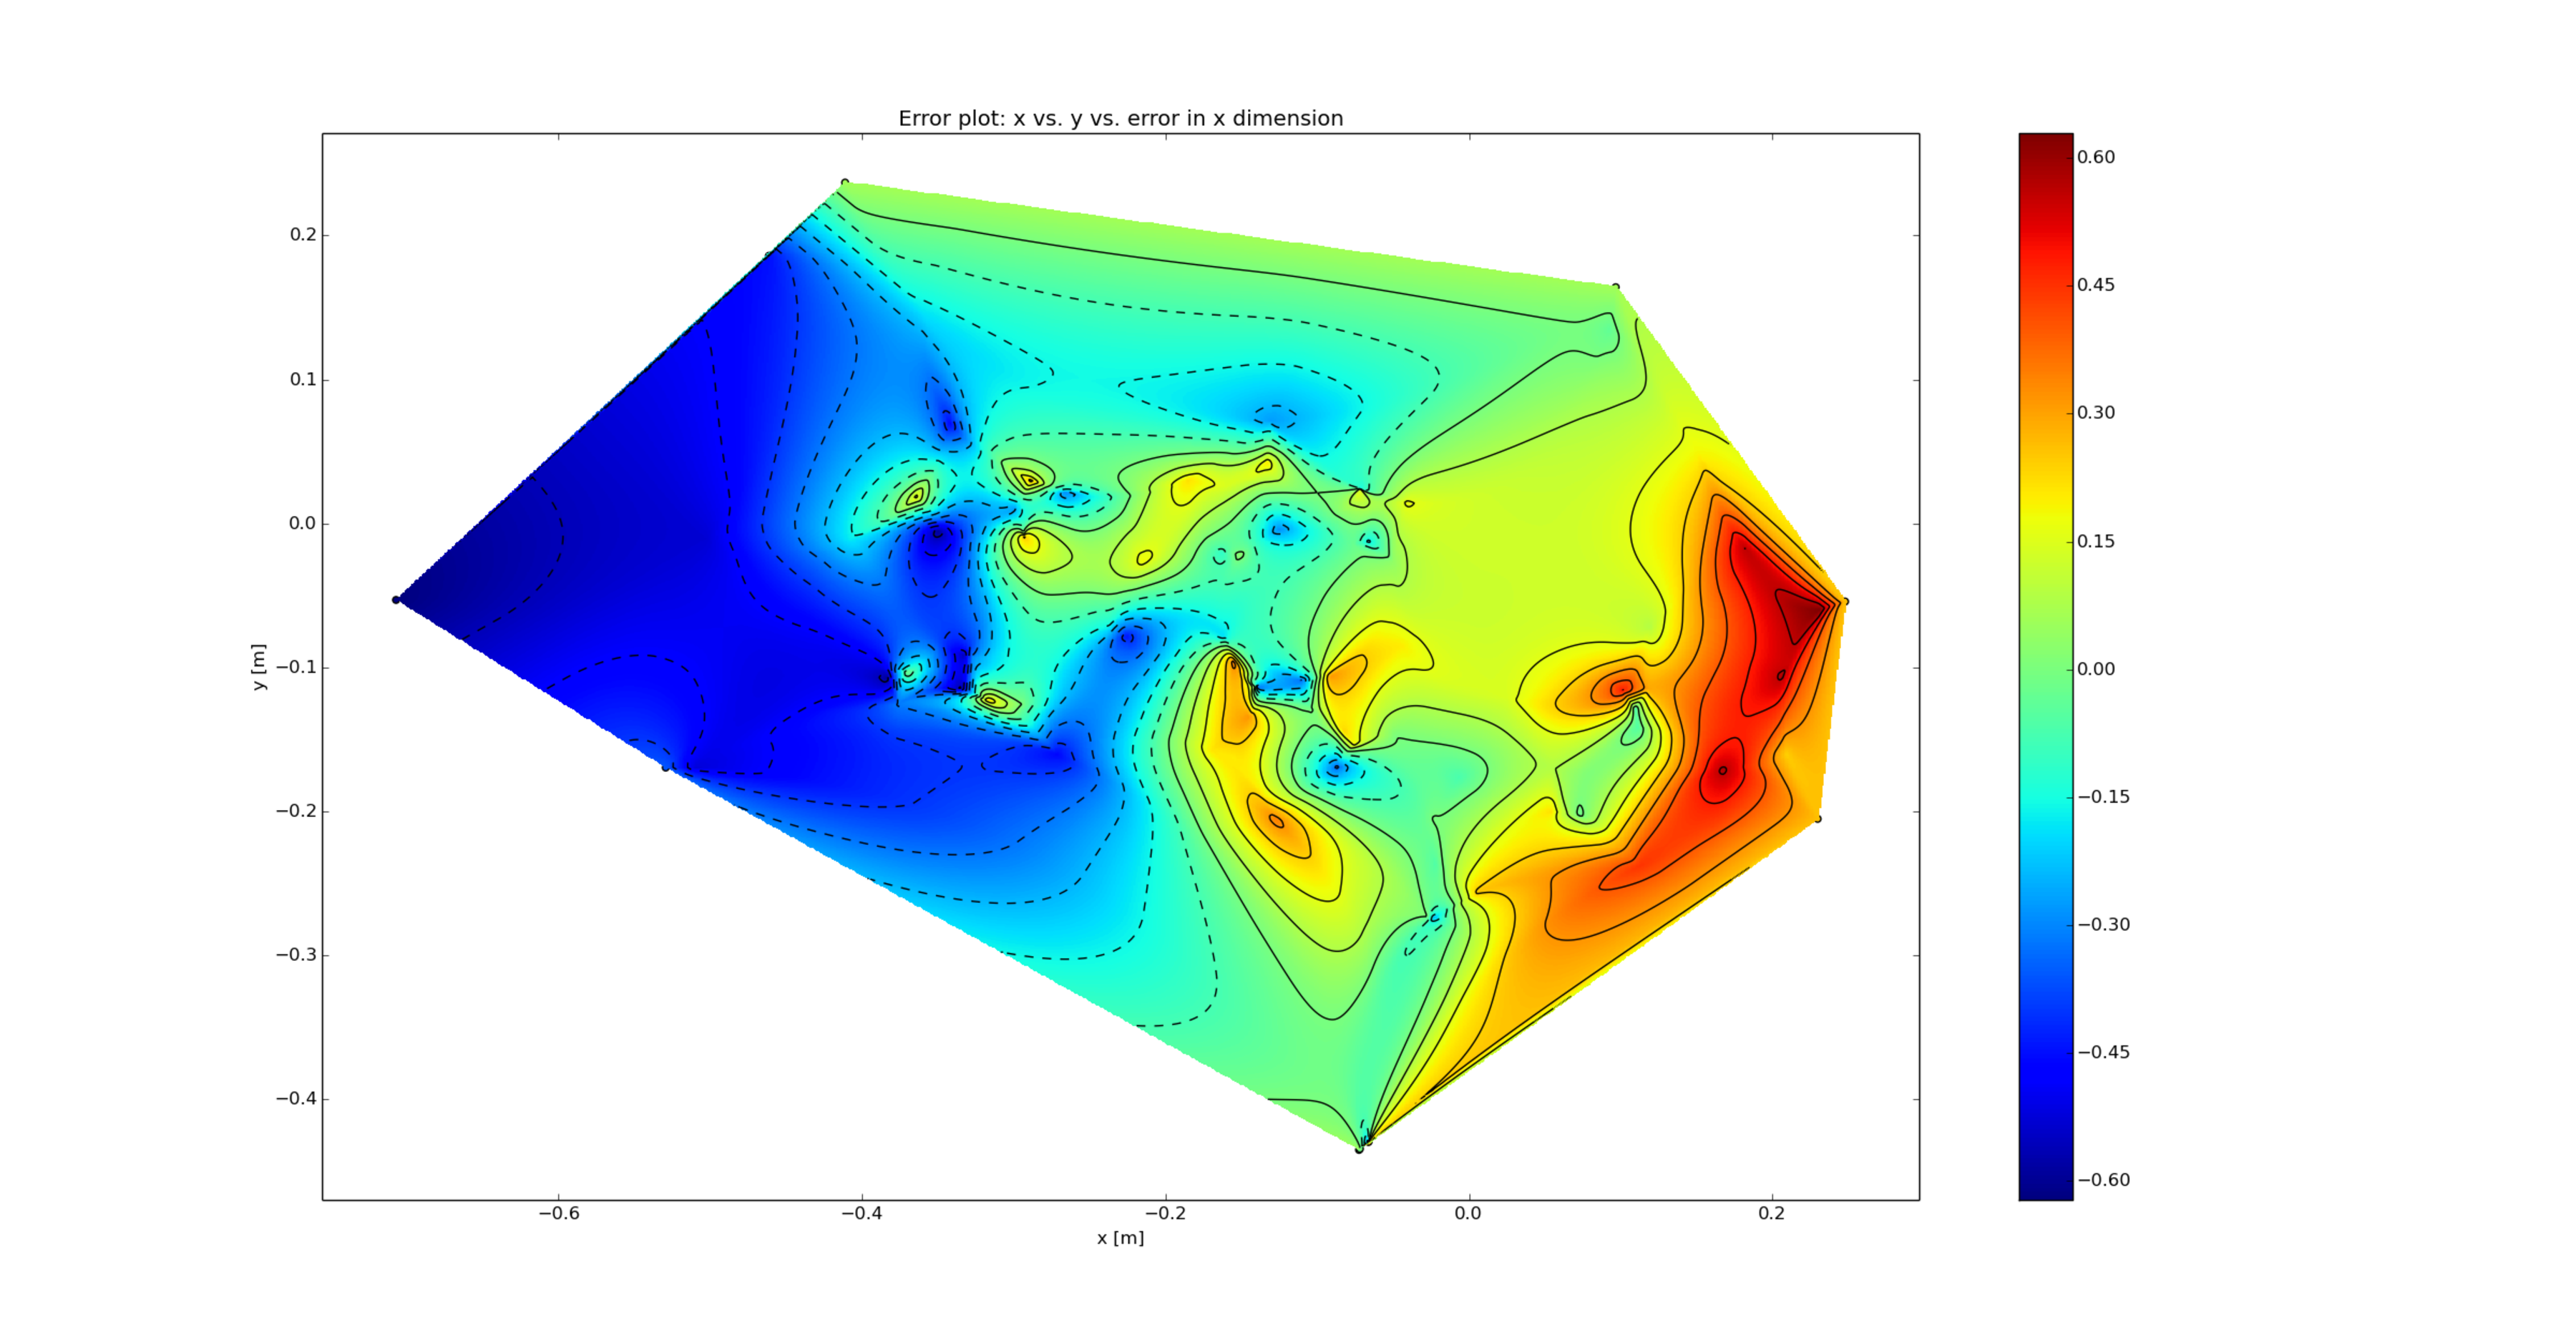
\includegraphics[clip, trim = 200 50 300 50, width=\textwidth]{figures/chapter3/contour_x}
    \caption{Contour plot of the error in the $x$ dimension over the $x-y$ plane.}
  \end{subfigure}
~
  \begin{subfigure}{0.31\textwidth}
    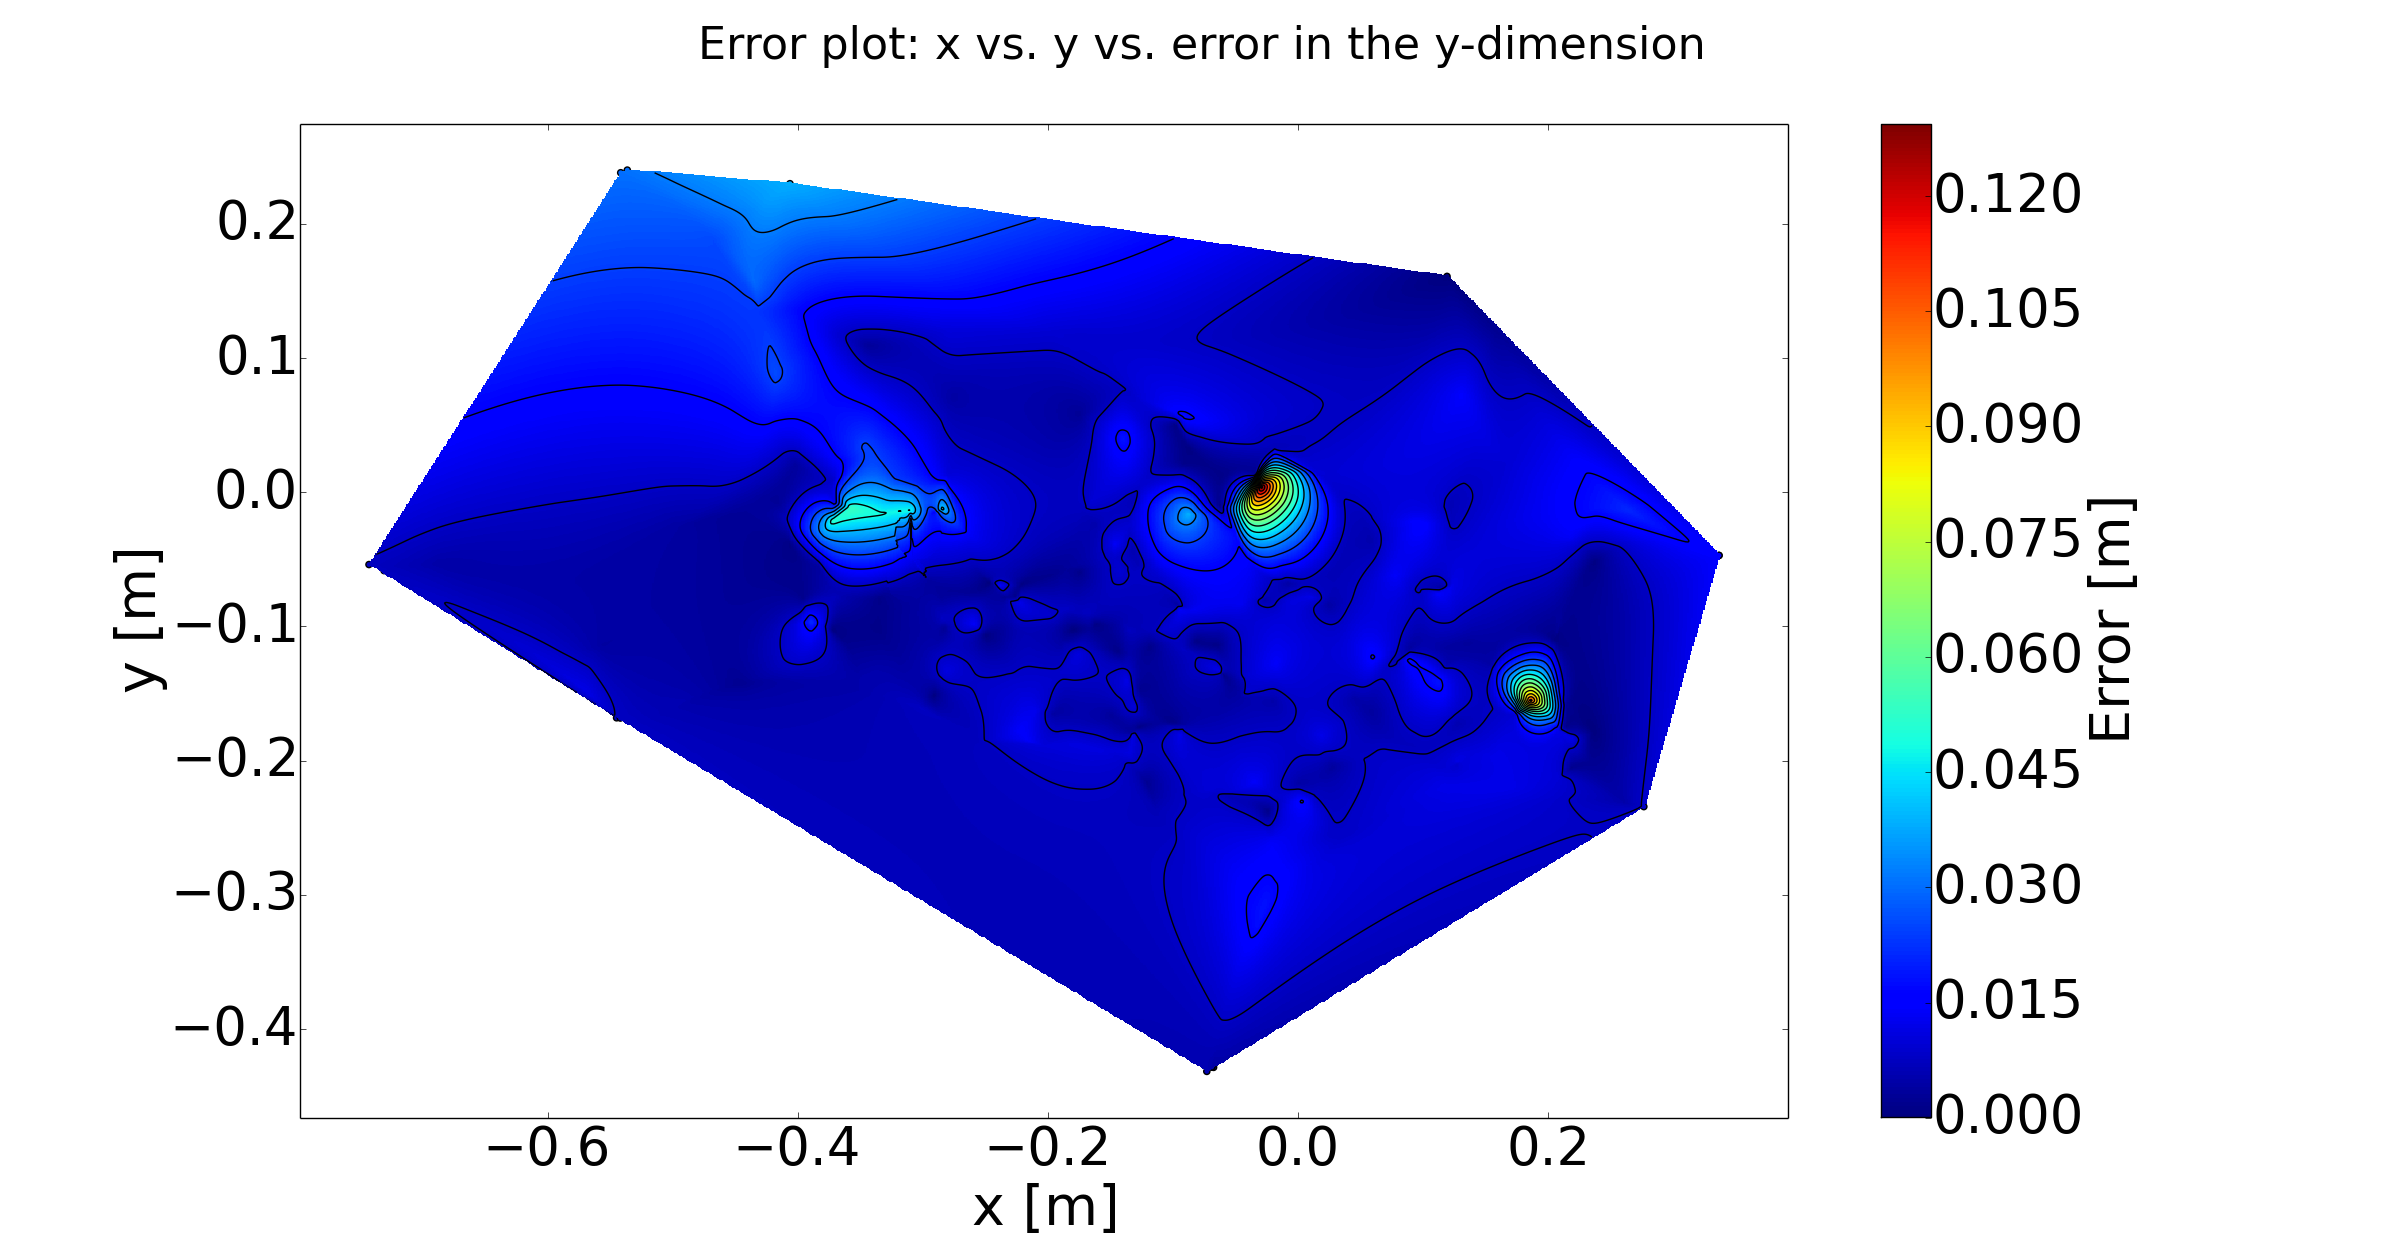
\includegraphics[clip, trim = 200 50 300 50, width=\textwidth]{figures/chapter3/contour_y}
    \caption{Contour plot of the error in the $y$ dimension over the $x-y$ plane.}
  \end{subfigure}
~
  \begin{subfigure}{0.31\textwidth}
    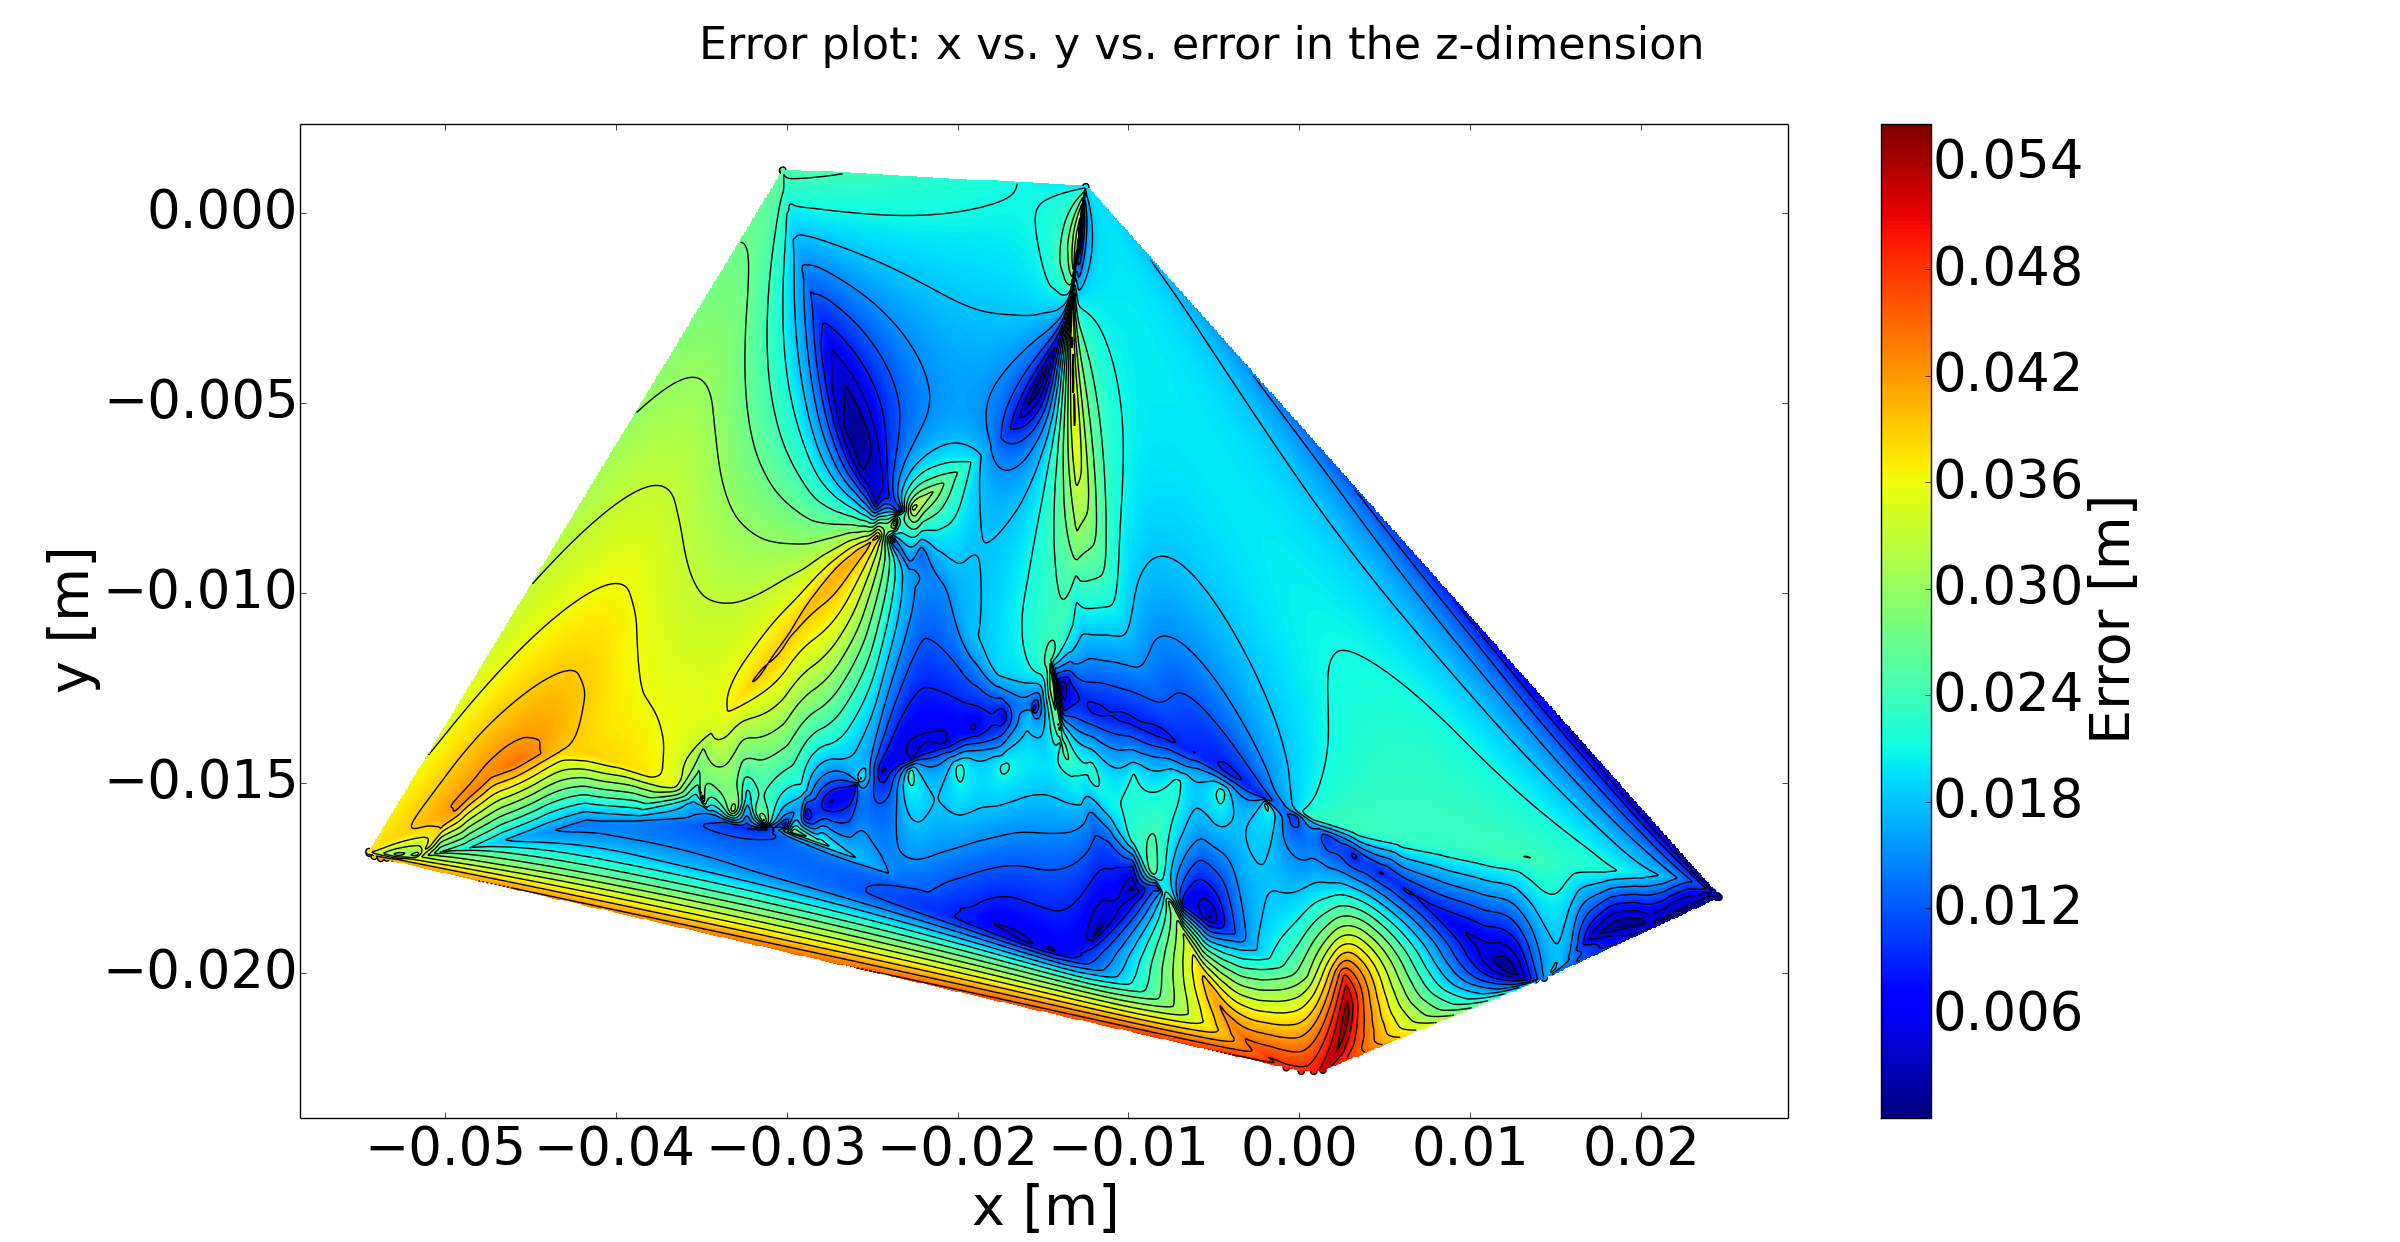
\includegraphics[clip, trim = 200 50 300 50, width=\textwidth]{figures/chapter3/contour_z}
    \caption{Contour plot of the error in the $z$ dimension over the $x-y$ plane.}
  \end{subfigure}
~
  \begin{subfigure}{0.31\textwidth}
    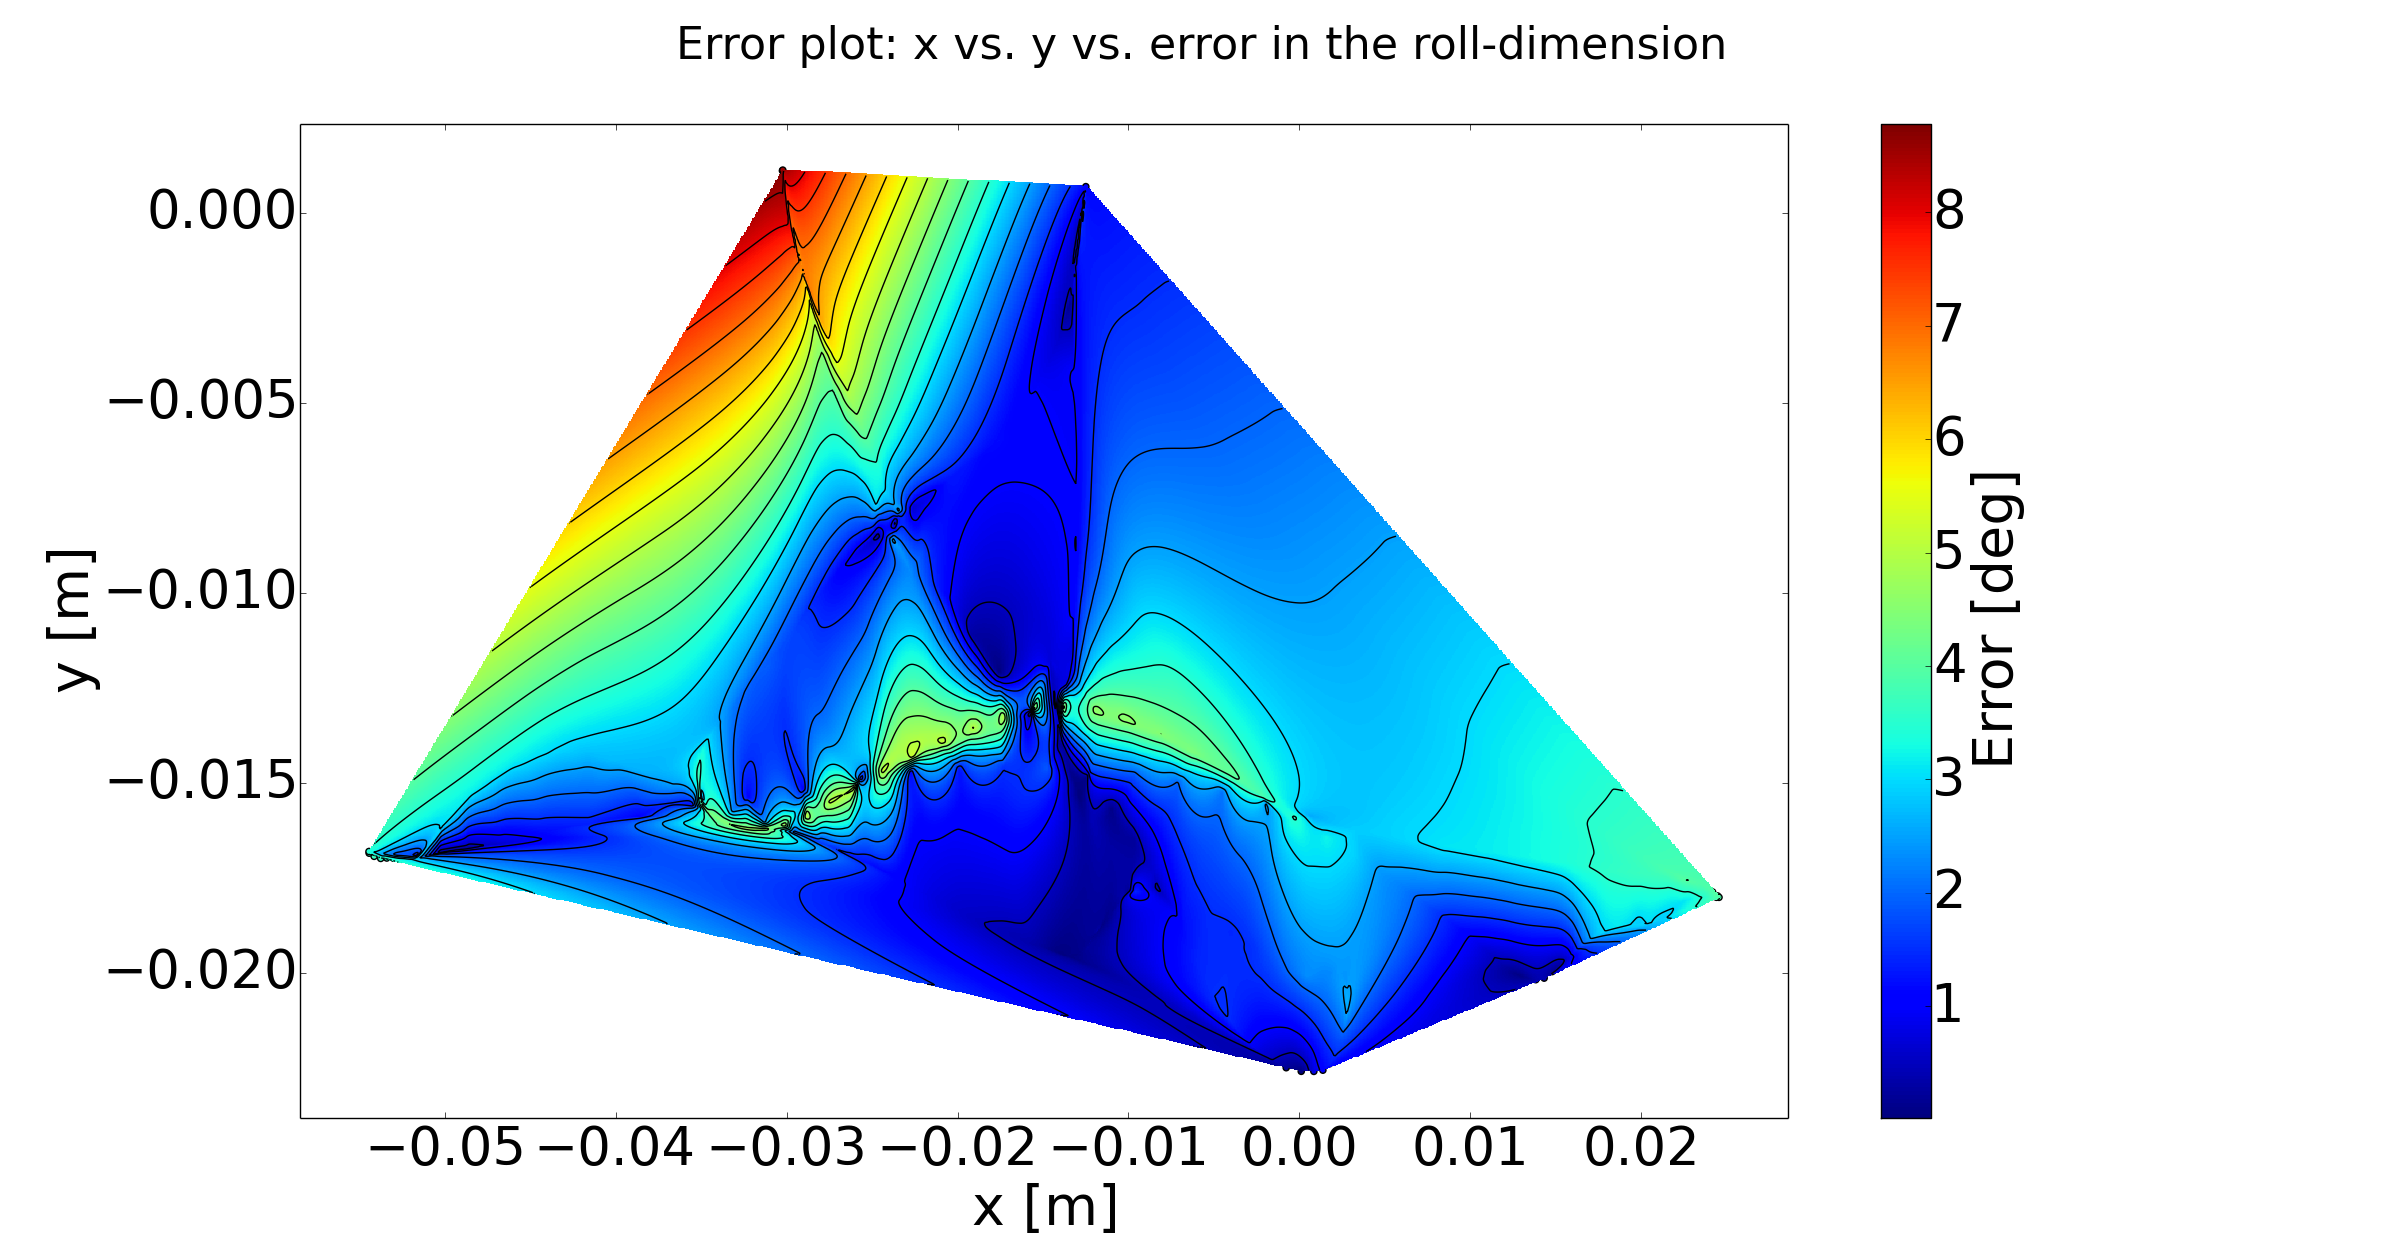
\includegraphics[clip, trim = 200 50 300 50, width=\textwidth]{figures/chapter3/contour_roll}
    \caption{Contour plot of the error in the $roll$ dimension over the $x-y$ plane.}
  \end{subfigure}
~
  \begin{subfigure}{0.31\textwidth}
    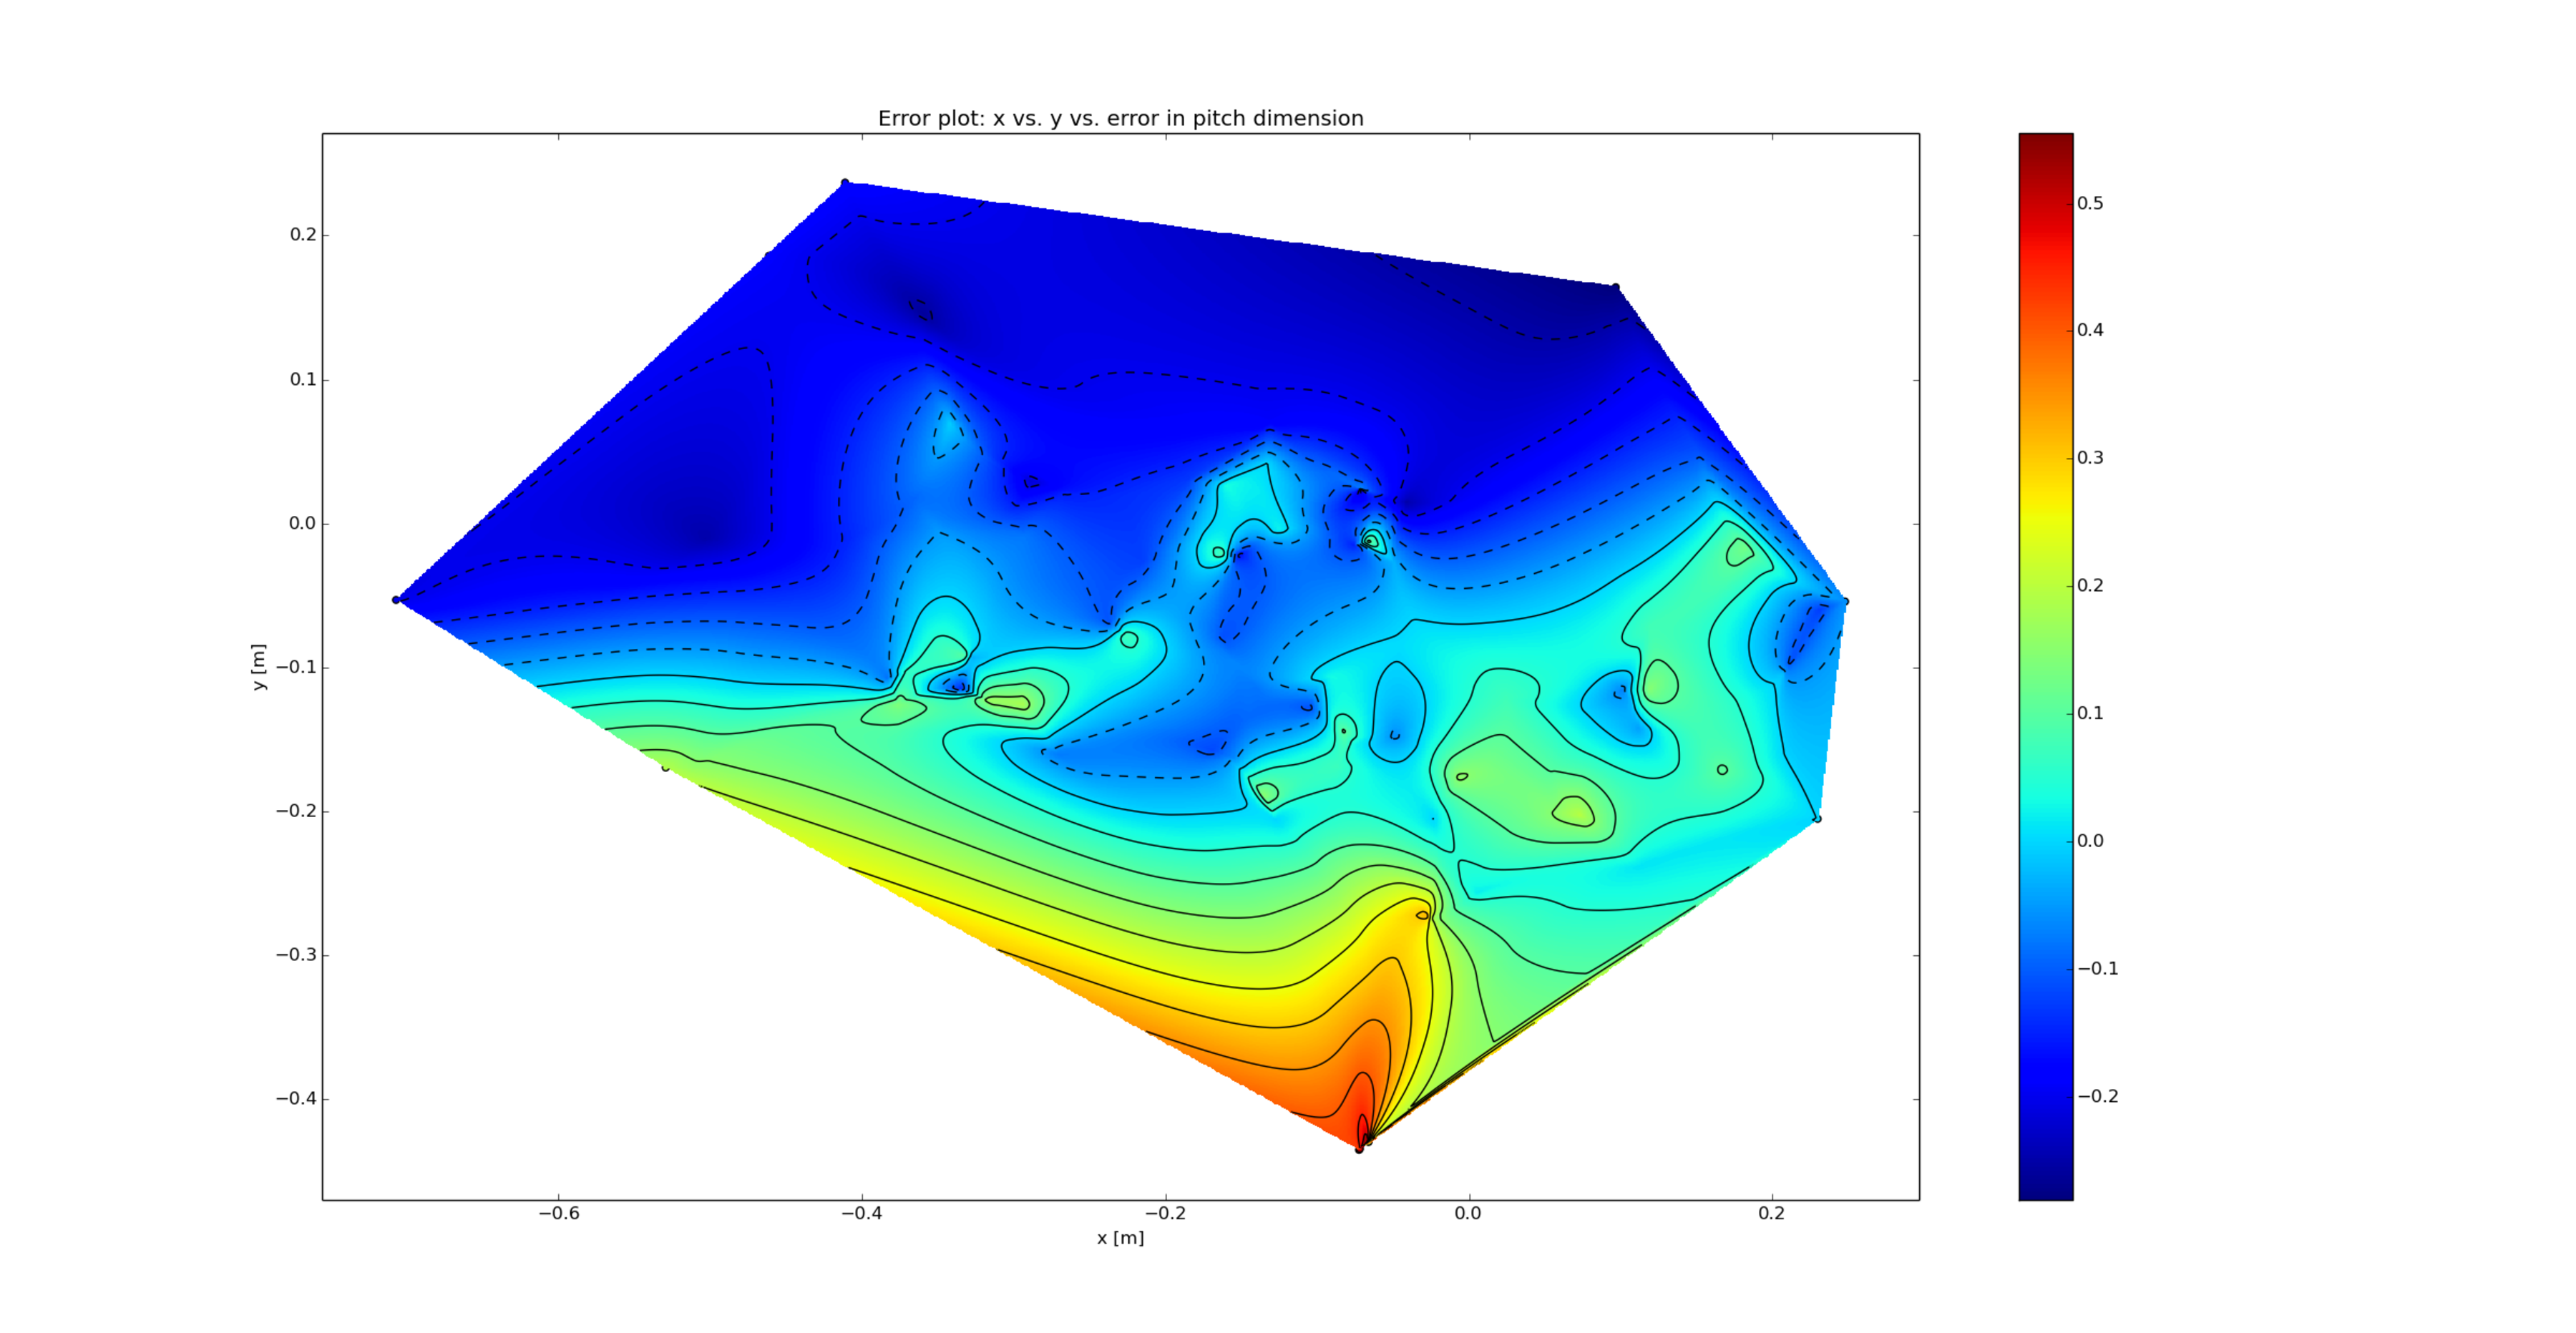
\includegraphics[clip, trim = 200 50 300 50, width=\textwidth]{figures/chapter3/contour_pitch}
    \caption{Contour plot of the error in the $pitch$ dimension over the $x-y$ plane.}
  \end{subfigure}
~
  \begin{subfigure}{0.31\textwidth}
    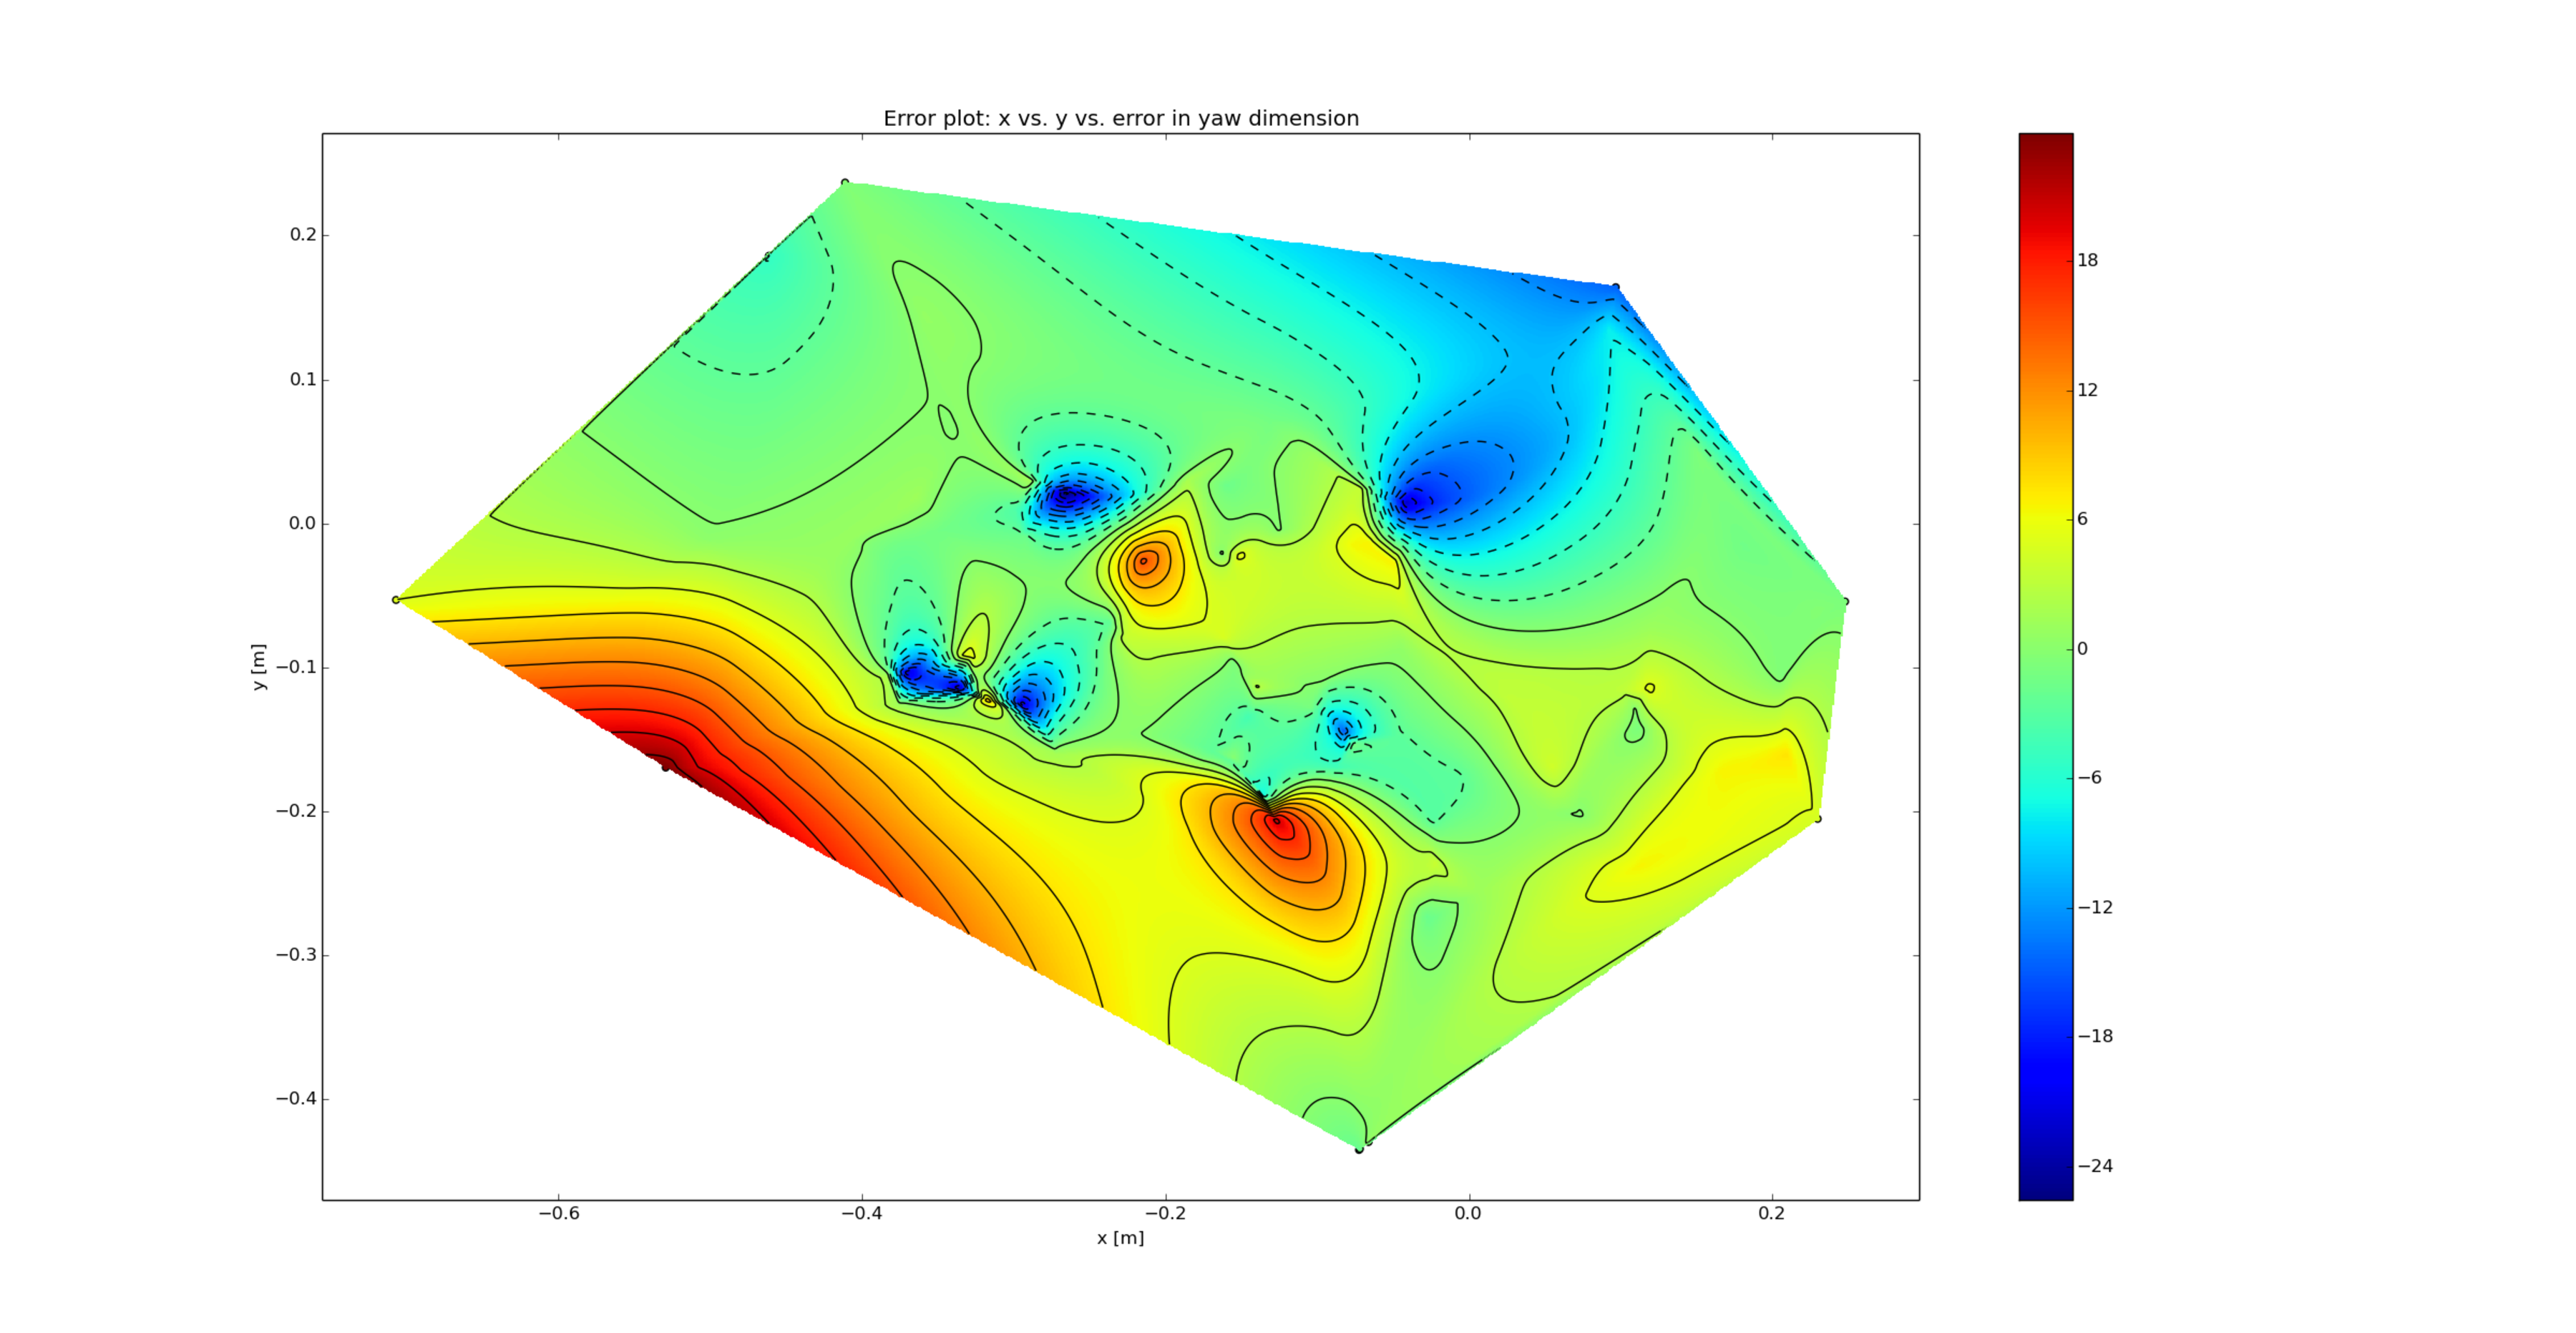
\includegraphics[clip, trim = 200 50 300 50, width=\textwidth]{figures/chapter3/contour_yaw}
    \caption{Contour plot of the error in the $yaw$ dimension over the $x-y$ plane.}
  \end{subfigure}
  \caption[A collection of contour plots of the translation and rotation vectors relative to one another]{A collection of contour plots of the translation and rotation vectors relative to one another. The units for the translation figures are in metres, and in degrees for the rotation figures. }
  \label{fig:err-contour}
\end{figure*}

From Figure~\ref{fig:err-contour} it can be seen that the error in a dimension varies when the two other pose dimensions changes. 

These plots, as well as the covariance matrix $\bm{\Sigma}$ indicates that there is no clear indication on the accuracy of the CVS, since its a function of the pose of the calibration board relative to the CVS's camera. 

\section{Conclusion}

In this chapter, the design and layout of a computer vision measurement system (CVS) was discussed. The system consists of hardware and software components and the details of both were discussed. The system was tested in an indoor measurement facility to determine its measurement accuracy. With the ground-truth measurements produced by this indoor system, it was possible to optimise the intrinsic camera parameters and improve the pose data from the CVS.

It was shown that the error data is a function of the pose of the calibration board relative to the CVS's camera. This constant error variation makes difficult to determine the measurement accuracy of a sample pose vector from the CVS.\@ The measurement accuracy of the CVS is very important and cannot be ignored. Therefore, another approach to determine the measurement accuracy was taken and was investigated. 
